%=================================================================
%				preamble
%=================================================================
\documentclass[11pt,letterpaper]{book}

\newcommand{\theauthor}{Thomas Graf}		        
\newcommand{\university}{Stony Brook University}	
\newcommand{\emailaddress}{lin630@thomasgraf.net}
\newcommand{\coursenumber}{Lin630}
\newcommand{\coursename}{Parsing and Syntactic Processing}
\newcommand{\thetitle}{\texorpdfstring{\coursenumber\\ \coursename}{\coursenumber --- \coursename}}
\newcommand{\thekeywords}{graduate level, research seminar, mathematical linguistics, syntax, Minimalist grammars}
\newcommand{\thedate}{}

\usepackage{mypackages}
\usepackage{mycommands}



%=================================================================
%			title format
%=================================================================
\author{\theauthor}
\title{\thetitle}
\date{\thedate}

%=================================================================
%			content
%=================================================================
\begin{document}
\raggedbottom
\pagestyle{empty}
\pagenumbering{Roman}
\maketitle
\tableofcontents

\setcounter{chapter}{-1}
\chapter{Syllabus}
\label{cha:syllabus}
\setcounter{page}{1}
\pagestyle{fancy}

\fcolorbox{gray!25}{gray!25}{
    \centering
    \begin{tabular}{l@{\qquad}l}
        \textbf{Course:} Parsing and Syntactic Processing &
        \textbf{Name:} Thomas Graf\\
        \textbf{Course\#:} Lin630 (officially still Lin651) &
        \textbf{Email:} lin630@thomasgraf.net\\
        \textbf{Time:} tbd &
        \textbf{Office hours:} tba\\
        \textbf{Location:} CompLab SBS N250&
        \textbf{Office:} SBS N249\\
        \textbf{Course Website:} \href{http://lin630.thomasgraf.net}{lin630.thomasgraf.net} &
        \textbf{Personal Website:} \href{http://thomasgraf.net}{thomasgraf.net}
    \end{tabular}
}

\section{Overview}
\begin{itemize}
    \item \textbf{Big Questions}
        \begin{itemize}
            \item What is the relation between competence and performance, grammar and parser?
            \item Are syntactic processing effects conditioned by the grammar?
            \item What qualifies as a parser as opposed to a recognizer or a parsing schema?
            \item Can we use insights from syntactic processing research to speed up current parsing technology?
        \end{itemize}
        %
        The first two are common questions for any processing course.
        The third and fourth one hint at the special twist of this course: we approach these issues from a computational perspective!
        Parsing theory is a big (albeit messy) area of computer science, there's tons of parsing models on the market.
        So let's bring all these insights to bear on how humans parse natural language.

    \item \textbf{Teaching Goals}\\
        At the end of this course you will 
        \begin{itemize}
            \item be familiar with a variety of common parsing models (top-down, bottom-up, left-corner, Earley, CYK)
            \item know the most common syntactic processing effects (in particular those related to memory usage)
            \item be able evaluate claims in the psycholinguistic literature from a computational perspective
        \end{itemize}

    \item \textbf{Prerequisites}\\
    None beyond basic syntax skills --- you should be able to draw a reasonable tree for a sentence like \emph{The fact that the employee who the manager hired stole office supplies did not go unnoticed by the janitor}.
    Knowledge of theoretical computational linguistics (e.g.\ as covered in Lin637) is helpful, but not necessary.
\end{itemize}

\section{Course Requirements}
\begin{itemize}
    \item \textbf{Homeworks}\\
        There will be weekly homeworks, the solutions of which will be discussed during review sessions run by students retaking this course.
        Homeworks are essential if you want to learn anything in this course --- you don't truly understand a parsing algorithm until you can carry it out yourself.
        %
    \item \textbf{Review Paper}\\
        Write a critical review of a particular topic in parsing or syntactic processing that will be shared with and commented on by your class mates.
        You have to get my approval for your topic and your list of readings by the end of week 8 (see the website for topic suggestions).
        Your paper should be about 15 pages (letter paper, 1in margins, double spaced, 12pt), must be written in \LaTeX, and has to be completed by the end of week 12.
        After you have gotten feedback from your colleagues, you must hand in a revised version by the end of finals week.

        This assignment serves two purposes: you get experience writing review articles, and your colleagues get to learn about topics that weren't covered in class.
        %
    \item \textbf{Paper Evaluations}\\
        %
        For each review paper, you have to write a 1-page evaluation (it can be longer if necessary, but do not go beyond 3 pages).
        Ideally, you should engage with the paper on an intellectual level, which means critiquing parts you disagree with, suggesting follow-up readings, or asking questions that were left unanswered.
        But presentational issues such as grammar, style, or overall structure can also be brought up.

        Think of this as you peer-reviewing a squib for a journal like \emph{Language and Linguistics Compass}, which is something you will have to do quite frequently as an academic.
        It also hones your skills for giving detailed but polite and structured feedback in a corporate environment, e.g.\ as part of writing and maintaining documentation for a specialized piece of software.
        %
    \item \textbf{Workload per Credits}
        %
        \begin{itemize}
            \item \emph{1 credit}: regular attendance, commenting on all review papers
            \item \emph{2 credits}: the above, plus doing all the homeworks
            \item \emph{3 credits}: the above, plus writing a review paper
        \end{itemize}
        %
        Students who are retaking this course for credit can instead volunteer to run some of the review sessions.
\end{itemize}

\section{Outline}

This outline assumes that we meet twice a week for 90 minutes with a 10 minute break, plus a weekly recitation of 60 minutes.
After week 9, we meet once a week for 60 minutes to brainstorm ideas for connecting parsing to protein folding.

\begin{center}
    \begin{tabular}{r@{\hspace{2em}}l@{\hspace{2em}}l@{\hspace{2em}}l}
        \toprule
        \textbf{Wk} & \textbf{Chap} & \textbf{Topic} & \textbf{Assignments}\\
        \midrule
        1 & \ref{cha:BigPicture},\ref{cha:ParserOverview} & Parsing across disciplines, modular view of parsing\\
        2 & \ref{cha:TopDown},\ref{cha:TopDownEval}       & Top-down parsing\\
        3 & \ref{cha:BottomUp},\ref{cha:ChartParsing}     & Bottom-up parsing, chart parsing intro\\
        4 & \ref{cha:ChartParsing}                        & CKY and Earley\\
        5 & \ref{cha:LeftCorner}                          & (Generalized) Left-corner parsing\\
        6 & \ref{cha:Semiring}                            & Semiring parsing\\
        7 & \ref{cha:BeyondCFG}                           & Moving beyond context-free grammars\\
        8 & \ref{cha:MG-TopDown},\ref{cha:StablerParser}  & CFG-parsing of mildly-context sensitive formalisms & get topic approved\\
        9 & \ref{cha:Deterministic},\ref{cha:Partial}     & LR parsing, partial parsing\\
        \midrule
        10 & & protein folding \\
        11 & & protein folding \\
        12 & & protein folding & review paper draft\\
        13 & & protein folding \\
        14 & & protein folding \\
        15 & & protein folding & paper evaluations\\
        \midrule
        finals1 & & Q\&A session\\
        finals2 & & & paper due\\
        \bottomrule
    \end{tabular}
\end{center}

\medskip
The whole course has a time investment of 3 credits for 15 weeks, which totals $3*53*15=2385$ minutes.
The distribution is shown below.
\medskip
%
\begin{center}
    \begin{tabular}{rrrr}
        \toprule
        \textbf{type}    & \textbf{number} & \textbf{minutes} & \textbf{total}\\
        \midrule
        lecture          & 18              & 80               & 1440\\
        recitation       & 9               & 60               & 540\\
        research meeting & 6               & 60               & 360\\
        Q\&A session     & 1               &                  & 45\\
        \midrule
                         &                 &                  & \emph{2385}\\
        \bottomrule
    \end{tabular}
\end{center}

\section{Policies}

\subsection{Contacting me}
\begin{itemize}
    \item Emails should be sent to \href{mailto://lin630@thomasgraf.net}{lin630@thomasgraf.net} to make sure they go to my high priority inbox.
        Disregarding this policy means late replies and is a sure-fire way to get on my bad side.
    \item Reply time $<24$h in simple cases, possibly more if meddling with bureaucracy is involved.
    \item If you want to come to my office hours and anticipate a longer meeting, please email me so that we can set aside enough time and avoid collisions with other students.
\end{itemize}

\subsection{Special Needs}
If you have any special needs that might impact your class performance (learning disabilities, impaired sight or hearing, etc.), please come to my office hours or contact me via mail so we can make suitable arrangements.


\section{Online Component}
Rather than Blackboard, I use github to distribute lecture notes and readings (yes, you have to print them yourself).
The readings are in a private repository, so you need a github account to access them.
If you don't have one already, you can create one for free (github does not collect any user data).
Make sure to email me your username asap so that I can give you access to the repository.
If you do not want to use github for some reason, you can drop by my office to make an offline copy of the readings.

\pagenumbering{arabic}
\pagestyle{fancy}
\chapter{The Big Picture: Why Parsing isn't Sentence Processing}
\label{cha:BigPicture}

On a purely technical level, parsing is the process of assigning a string of symbols a structural description according to some formal specification, usually a grammar.
As such, parsing is not specific to language, any kind of problem where hidden structure has to be inferred from linearly arranged items may be considered an instance of parsing.
This covers a very diverse range of processes such as discerning the structure of source code, segmenting a movie into its three acts, and even protein folding (the mechanism by which sequences of amino acids combine into these complex three-dimensional objects we call proteins).

This general view of parsing is possible thanks to the semantic agnosticism of formal languages: pretty much everything can be conceptualized as a formal language.
A program is a sentence of some programming language, and the programming language is defined via an alphabet (variables, functors, data structures, etc.) and a grammar that defines how the elements of the alphabet can be concatenated.
The set of well-formed proteins is also a language that is defined by an (unfortunately still unknown) grammar with amino acids as its alphabet.
And of course natural languages can be viewed as formal languages, as is commonly done in computational linguistics.
In this case, parsing is about assigning structures to natural language utterances. 

Linguists might interject that this description is overly general: natural language parsing must assign \emph{tree-like} objects to natural language utterances that match, in some suitably abstract sense, the structures subconsciously employed by native speakers.
This is indeed the standard view of parsing in linguistics, but it is a very specific notion that is tailored to an equally specific set of goals.
The linguistic definition treats parsing as a model of how humans process sentences.
That is certainly an interesting enterprise, but as the non-linguistic examples above demonstrate it is a particular subproblem of the full spectrum of parsing work.
In fact, human parsing has various quirks and peculiarities that distinguish it from pretty much every other parsing problem.
So we should be careful to distinguish the formal process of \emph{parsing} from the cognitive mechanisms driving \emph{sentence processing}.

As we will see, though, the two have a fair share of overlap, so that results about the former can inform the latter.
That is highly welcome; sentence processing is a lot murkier than parsing, and whenever one ventures into murky territory, it is advisable to have some landmarks as points of orientation.

\section{Parsing in Computer Science}
\label{sec:BigPicture_CS}

\subsection{Goals and Applications}
\label{sec:BigPicture_CS-Goals}

Computer scientists were interested in parsing from an early date on, with \citet{Yngve55} usually cited as the first worked-out parsing algorithm.
To put this into perspective, research in formal language theory did not take off until \cite{Chomsky56} and \citet{ChomskySchuetzenberger63}.
So parsing research was being done before its formal foundation was even in place yet (as is almost always the case in the history of science).

Quite typical for computer science, the interest in parsing wasn't driven by intellectual curiosity alone but had a strong applied component to it.
The early 50s had seen the arrival of high-level programming languages like Autocode, which was soon followed by Fortran and COBOL\@. 
This made it possible to write programs in a language that abstracts away from the machine code actually executed by the computer.
It is hard to imagine nowadays just how revolutionary high-level programming were at the time.
Their most obvious advantage is that they are much easier to understand for humans, which enables them to write and maintain much more complicated programs with less time and effort. 
But by abstracting away from the hardware executing the code, high-level programming languages also made it possible to write programs that can run on very different hardware.
Not all computers are the same --- your laptop's x86 architecture shares little with your tablet's ARM-based hardware, yet you can write some Python code that will immediately run on both without any system-specific modifications because Python, just like any other high-level programming language, is deliberately designed to be hardware agnostic.
These were undeniable advantages of high-level programming languages, but as so often in life they also created new problems.

While high-level programming languages do away with the need for humans to write code ``close to the metal'', that does not change the fact that the actual hardware can only understand instructions in its own machine code.
Somehow, the human-friendly source code has to be translated into hardware-friendly machine code, which is commonly referred to as \emph{compilation} or \emph{compiling}.
Compiling is anything but straight-forward as even the most elementary programming concepts like variables pose serious challenges.
Consider the following piece of Python code.
%
\begin{center}
    \pythonfile[firstline=4]{./code/misc/variable_scope.py}
\end{center}
%
This code involves two assignments of the variable $a$.
One occurrence of $a$ is initialized as the integer $1$, the other one is set to $2$ in the definition of the \verb|increment_by_two| function.
A careless translation of this program might overwrite the first instantiation of $a$ by the second one and would thus compute $2+2$ rather than the intended $1+2$.
The actual translation for Python, on the other hand, is smart enough to recognize that the second variable appears within the scope of a function and thus constitutes a different object that just happens to have the same name.
But scope is a structural notion, it is not readily apparent from the linear order of symbols.
For example, if we added another assignment for $a$ immediately after the function, that should overwrite the first occurrence of $a$. 
Structural considerations like this are indispensable for a correct compilation procedure from high-level source code to hardware-suitable machine code, and as a result, an efficient method for parsing source code is a prerequisite for compiler design.

Since parsers main purpose in computer science is to facilitate the compilation of source code into machine code, it is of utmost importance that parsers are not ill-behaved.
On a practical level, parsers must be efficient --- you don't want your OS to crash because the parser swallowed up all your memory while reading in your program, and compiling even large programs with millions of line of code like the Linux kernel should not take unfeasibly long.
In addition, a parser should not assign a program an illicit structure or fail to find a structure for a well-formed program.
The technical term for this is \emph{correctness}, which is formally defined as the conjunction of soundness and completeness.
%
\begin{description}
    \item[Soundness] If the parser assigns string $s$ structure $\sigma$, then $\sigma$ is a licit structure for $s$.
        In plain English: The parser says only correct things.
    \item[Completeness] If $\sigma$ is a licit structure for string $s$, then the parser assigns $\sigma$ to $s$.
        In plain English: The parsers says all correct things.
\end{description}

Note that soundness and completeness presuppose that we can tell for a given string what its licit structures are.
That means we need a definition of the class of well-formed structural descriptions.
In other words, we need a grammar.

\subsection{Rewrite Grammars}
\label{sub:BigPicture_Grammars}
The class of structural descriptions the parser has to operate in is supplied by a \emph{rewrite grammar} $G \is \tuple{N, T, S, R}$, where
%
\begin{itemize}
    \item $N$ is a finite, non-empty set of \emph{non-terminal} symbols, and
    \item $T$ is a finite, non-empty set of \emph{terminal} symbols, and
    \item $S \in N$ is the designated \emph{start} symbol,
    \item $R \subset (N \cup T)^* \cdot N \cdot (N \cup T)^* \times (N \cup T)^*$ is a finite set of rewriting rules.
\end{itemize}
%
In linguistic parlance: the grammar has lexical items ($= N$), parts of speech ($=T$), a special part of speech ($=S$), and a number of rules for rewriting (the set of which is called $R$).
The rules are usually written in the form $\alpha \rewrite \beta$ to indicate that $\alpha$ is rewritten as $\beta$.
The definition above puts no restrictions on $\alpha$ and $\beta$ except that they are strings of symbols drawn from $N$ and $T$, and $\alpha$ must contain at least one non-terminal.
A grammar generates all those strings that can be obtained from the start symbol $S$ by applying rewrite rules until the output consists only of terminal strings.
If string $s$ is generated by grammar $G$, we also say that $G$ \emph{derives} $s$.
The \emph{language generated by $G$} is the set $L$ of strings that $G$ derives.
%
\begin{examplebox}[A Rewrite Grammar in Action]
    Suppose we have a grammar $G$ with $T \is \setof{a,b,c,d}$, $N \is \setof{A,B}$, and start symbol $A$.
    Furthermore, $R$ consists of the following rules:
    %
    \begin{center}
        \begin{tabular}{rrcl@{\hspace{5em}}rrcl}
            1) & A  &\rewrite & a & 4) &  A & \rewrite & AA\\
            2) & B  &\rewrite & b & 5) &  A & \rewrite & Bc\\
            3) & AB &\rewrite & a & 6) & aB & \rewrite & d\\
        \end{tabular}
    \end{center}

    This grammar generates an infinite set of strings (why?).
    Here's three of them and how the grammar derives them:

    \[
        A
        \rewriteR{4} AA 
        \rewriteR{5} ABc
        \rewriteR{3} ac
    \]
    \[
        A
        \rewriteR{4} AA
        \rewriteR{5} ABc
        \rewriteR{1} aBc
        \rewriteR{6} dc
    \]
    \[
        a
        \rewriteR{4} AA
        \rewriteR{4} AAA
        \rewriteR{4} AAAA
        \rewriteR{5} ABcAA
        \rewriteR{3} acAA
        \rewriteR{5} acABc
        \rewriteR{1} acaBc
        \rewriteR{6} acdc
    \]
\end{examplebox}

By default, rewrite grammars are not particularly well-behaved on a computational level --- for instance, some of them are so complex that one cannot tell for all strings whether they are generated by the grammar.
This immediately entails that they do not have efficient parsers, either.
After all, the parser has to assign a structure to every string according to the rewrite grammar, and if it could do that for every string, it could also determine for every string whether it is actually generated by the grammar (since an ``ungrammatical'' string would have an illicit structure).
%
\begin{proposition}
    Parsing is impossible for unrestricted rewrite grammars.
\end{proposition}

For this reason, computer scientists prefer a subclass of rewrite grammars known as \emph{context-free grammars} (CFGs).
In syntax, those are commonly known as \emph{phrase structure grammars} (PSGs).
For CFGs, $R$ is a finite subset of $N \times (N \cup T)^+$, that is to say, only a single non-terminal symbol can appear to the left of a rewrite arrow.
That's why these grammars are called context-free: whether a rule can apply to a non-terminal symbol never depends on what appears to the left or the right of the symbol.
%
\begin{exercise}
    The grammar in the previous example has four context-free rewrite rules.
    What are they?
\end{exercise}
%
\begin{examplebox}[A Context-Free Grammar]
    Let $G \is \tuple{
            \setof{S},
            \setof{a,b},
            S,
            R}$,
    where $R$ contains the following rewrite rules:
    %
    \begin{align*}
        S &\rewrite aSb\\
        S &\rewrite ab
    \end{align*}
    %
    This grammar generates an infinite set of strings, including $\String{aaabbb}$:
    %
    \[
        S
        \rewrite \String{aSb}
        \rewrite \String{aaSbb}
        \rewrite \String{aaaSbbb}
    \]
    Can you give a description of the language generated by $G$?
\end{examplebox}

The nice thing about CFGs is that their derivations can be represented in terms of trees.
So originally the phrase structure trees used in syntax were actually the derivation trees of CFGs (we will come back to this point much later in the semester during our discussion of Minimalist grammars).
%fixme: chapter reference
%
\begin{examplebox}[CFG Derivation Trees]
    The context-free derivation above corresponds to the tree below:
    %
    \begin{center}
        \begin{tikzpicture}
            \Tree
                [.S
                    a
                    [.S
                        a
                        [.S
                            a
                            b
                        ]
                        b
                    ]
                    b
                ]
        \end{tikzpicture}
    \end{center}
\end{examplebox}
%
\begin{exercise}
    In linguistics there are many debates about the difference between \emph{representational} and \emph{derivational theories}.
    Representational theories do not care about how structures are assembled and instead use constraints to separate the well-formed structures from the ill-formed ones.
    Derivational theories describe how the structures built via certain operations and restrict when and where these operations may apply.
    Phrase structure trees are usually thought of as representational in nature, they encode the structure of the sentence but not necessarily how it was built (e.g. via Merge and Move in Minimalism).
    What should we make of this divide given that phrase structure trees were originally derivation trees?
\end{exercise}


\subsection{Recognizers and Parsers}
\label{sub:BigPicture_Parsing}

In many applications it isn't important to know the structure of an input string but just whether it is well-formed or not.
A \emph{recognizer} is a formal device (e.g.\ a piece of software, but we could also build an analog machine) that can tell for every string whether it is generated by a specific grammar $G$.
A \emph{parser} is an extension of a recognizer in that it not only determine for a given string $s$ whether it is generated by $G$, but if $s$ is generated by $G$, then the parser also assigns $s$ a structural description according to the grammar.
To linguists the distinction may seem pedantic since intuitively there is no way to determine the well-formedness of a sentence without analyzing its structure;
when we ask speakers for grammaticality judgments, we ask them whether there is a well-formed structure for the sentence.
This is also true of recognizers to some extent as they do reason based on the structural regularities inherent to the supplied grammar, but a recognizer does not necessarily keep track of the structure it builds.
Think of it this way: if I ask you whether $1+2+3+4 = 10$, you can confirm this without keeping track whether you first added $1$ and $2$, or $2$ and $3$, or maybe something completely different.
Similarly, a recognizer only needs to determine whether a string is generated, not how it is generated --- that is the parser's job.

% In general, recognizers are designed in a modular fashion such that they are not restricted to a single grammar but instead work for an entire class of grammars.
% So a recognizer for CFGs takes a CFG $G$ as a parameter and then determines for a given string whether it is generated by $G$ (strictly speaking, we should call such a parameterized recognizer a meta-recognizer since it is actually a program that computes a recognizer for the supplied grammar).
%
% In computer science, this usually means assigning the string its derivation tree.
As you might have guessed already, it is often very easy to extend a recognizer into a parser by simply keeping track of the steps the recognizer uses to determine whether a string is in the grammar's language since these steps are closely related to the grammar's rewrite rules.
Things get tricky, though, when a string has more than one derivation tree.
Should the parser assign all derivations or only one, and if the latter, which one?
There's different solutions for this scenario, and we will encounter some later in the semester.

\begin{remark}
    Strings with multiple derivations are rare in computer science because most parsing is concerned with parsing computer programs, i.e.\ taking a piece of source code and determining its underlying structure to facilitate the translation of the program into machine code.
    And programming languages are deliberately designed in such a way that every well-formed string has one unique derivation (although there is sometimes local ambiguity which can only be resolved after reading in a few more symbols).
\end{remark}


\section{Syntactic Processing}
\label{sec:BigPicture_Processing}

\subsection{The Human Parser and its Quirks}
\label{sub:BigPicture_HumanParser}
From the perspective of a computer scientist, whatever controls syntactic processing is a very unruly piece of machinery.
First of all, it does not seem to be complete. 
\emph{Garden path sentences}, for example, are well-formed yet so hard to process that most native speakers can't do it without help from a friendly linguist.
%
\begin{exe}
    \ex
    \begin{xlist}
        \ex The horse raced past the barn fell.
        \ex The old man the boat.
        \ex The government plans to raise taxes were defeated.
    \end{xlist}
\end{exe}
%
Soundness doesn't hold, either, since speakers commonly fall prey to \emph{grammatical illusions}.
%
\begin{exe}
    \ex
    \begin{xlist}
        \ex The key to the cabinets are on the table.
        \ex The candidates that no republicans nominated have ever won.
        \ex More people have been to Russia than I have.
    \end{xlist}
\end{exe}
%
And excessive memory load is frequent, but seems to depend more on the structure of a sentence rather than its length.
In each one of the following pairs, the first sentence is a lot easier than the second even though they have the same length \citep[cf.][]{Gibson98, Resnik92}.
%
\begin{exe}
    \ex
    \begin{xlist}
        \ex The cheese was rotten that the mouse ate that the cat chased. 
        \ex The cheese that the mouse that the cat chased ate was rotten.
    \end{xlist}
    \ex
    \begin{xlist}
        \ex The fact that the employee who the manager hired stole office supplies worried the executive.
        \ex The executive who the fact that the employee stole office supplies worried hired the manager.
    \end{xlist}
\end{exe}

Furthermore, processing effects can vary across languages.
For instance, modification of nested phrases is often ambiguous.
%
\begin{exe}
    \ex I fixed the door of the car with a scratch.
\end{exe}
%
Here the PP \emph{with a dent} can modify \emph{window} or \emph{car}.
Some languages like English prefer modification of the structurally more embedded noun \emph{car}, while German and Spanish speakers are more likely to interpret the sentence as \emph{scratch} modifying the higher noun \emph{door}.
These two readings are referred to as low and high PP attachment, respectively.
So not only is the human parser a rather ill-behaved creature from a computational perspective, it isn't even a uniform creature across languages.

But hold on a second.
Soundness and completeness are properties that hold with respect to a specific grammar.
That's straight-forward in computer science, where the roles of grammar and parser are well-defined.
With natural language, on the other hand, we have no idea what the real thing looks like.
So does it make any sense to carry over the computer scientists' strict division between grammar and parser?

\subsection{Three Cognitive Oppositions}
\label{sub:BigPicture_Oppositions}
The distinction between grammar and parser is commonly conflated with the competence-performance dichotomy that was introduced in chapter 1 of \emph{Aspects} \citep{Chomsky65}.
%
\begin{description}
    \item[Competence] A speaker's linguistic ability and knowledge, abstracted away from all cognitive, anatomic and physical limitations (e.g.\ memory limitations, a brain aneurysm, or the finite time span afforded by a universe that's doomed to eventually collapse in on itself)
    \item[Performance] A speaker's usage of his linguistic knowledge.
\end{description}
%
Equating competence with grammar and performance with parsing is indeed tempting, seeing how the quirks of the human parser can limit a speaker's ability to understand a sentence in real time even if its structure quickly emerges upon careful inspection.
The parser is indeed a factor that one needs to abstract away from if one wishes to describe a speaker's knowledge of language.

But the distinctions are not exactly the same.
This is easy to see once one considers the fact that the competence performance distinction can be applied to a parser itself.
The competence theory of the parser is a specification of the parser and its behavior under ideal conditions --- some kind of algorithm or program, not too different from how one specifies a parser for a programming language.
The performance theory, on the other hand, is about how the parser behaves once it is run in the cognitive environment of the human brain.
The leading idea of this course is that we can import competence theories of parsing from computer science and turn them into performance theories of parsing via some linking hypothesis, some metric that relates the parser's behavior to processing difficulty.

Depending on how much of a scientific realist you are (personally I'm closer to a constructive empiricist in the vein of \citealt{Fraassen80}), you might wonder what this view implies about language as a cognitive module \citep[cf.][]{Chomsky86a, Fodor83}.
Are the grammar and the parser two distinct cognitive systems?
Should we distinguish the competence parser from the performance parser?
The short answer is that this doesn't matter for this course.
The rude answer is that this is pointless philosophizing and you're better off spending your time on real research.
And then there's a long answer in terms of \emph{Marr's three levels of analysis} \citep{MarrPoggio76}.

Marr proposes that any aspect of cognition can be described on three levels of increasing abstraction:
%
\begin{description}
    \item[physical] the ``hardware'' instantiation, e.g.\ neural circuitry for vision
    \item[algorithmic] what kind of computations does the system perform, what are its data structures and how are they manipulated
    \item[computational] what problem space does the system operate on, how are the solutions specified
\end{description}
%
\begin{examplebox}[Set Intersection on Three Levels]
    Suppose you have two sets of objects, $A$ and $B$, and you want to write a computer program that tells you which objects belong to both sets.
    \begin{itemize}
        \item On a computational level, that program is easily specified: it takes two sets as input and returns their intersection ($A \cap B$).
        \item On the algorithmic level, things get trickier.
        For instance, what kind of data structure do you want to use for the input (sets, lists, arrays?), and just how does one actually construct an object that's the intersection of two sets?
    \item On the physical level, finally, things are so complicated that it's basically impossible to tell what exactly is being computed by the machine.
        Voltages increase or decrease in various transistors spread over the CPU, memory and mainboard, and that's about all you can make out.
        Unless you already have a good idea of the higher levels and the computational process being carried out, it's pretty much hopeless to reverse engineer the program from the electrical signals.
    \end{itemize}
\end{examplebox}
%
Marr's levels of analysis highlight that one and the same object can be described in very different ways, and all three levels are worth studying.
A computational specification can be implemented in various distinct ways on the algorithmic level, and algorithms can be realized in a myriad of physical ways --- for instance, your laptop and your tablet use very different processor architectures (x86 and ARM, respectively), but a Python program will run just fine on either platform despite the differences in electric signals.
And of course this hierarchy is continuous: Assembly code is closer to the physical level than C, which in turn is closer to it than Python.
However, the more you are interested in stating succinct generalizations, the more you'll be drawn towards abstractness and hence the computational level at the top of the continuum.

What does this mean for language?
Instead of thinking of the grammar and the parser as distinct entities, we can view them as different descriptions of the human faculty of language, with the grammar close towards the top in the computational section, while the parser is closer to the algorithmic level \citep[cf.][]{NeelemanKoot10}.
The distinction between competence parser and performance parser would also fit into this paradigm, with the former closer to the computational level but not as close as what we call the grammar.

\begin{exercise}
    Can you think of an experiment or case study that would argue against the idea of parser and grammar as one and the same object?
\end{exercise}


\subsection{Why Processing Matters}

Given what we have seen so far, the waters of syntactic processing are indeed very murky.
Why, then, should we bother with syntactic processing at all rather than just focusing on computational parsing models and their usage in real-world applications?
As so often in science, the most natural and immediate answer is that syntactic processing is an interesting and fun puzzle.
And just like other aspects of human psychology studying it comes with the satisfaction of feeding mankind's innate vice of anthropocentric narcissism.
But there are more tangible advantages.

For those that mostly care about the engineering aspects of language technology, the human parser is both a challenge and an opportunity.
It is a challenge because the limitations of the human parser are limitations of what is comprehensible to humans.
A natural language system with perfect command of English will be considered broken by its user's if it expresses itself in garden path sentences and with multiple levels of center embedding.
These constructions might not be particularly hard for a formal parsing model, but they nonetheless must be avoided in interactions with humans.
Studying syntactic processing is also an opportunity because history has shown that many a great engineering insight can be gleamed from nature, and the human parser is an impressive machine --- warts and quirks notwithstanding.
The parser is incredibly robust for most sentences encountered in the wild, and it operates much faster than any known parsing algorithm.
It is essentially real-time, which means that if the input is presented to the parser in an ongoing stream, the parser finishes within some fixed constant $c$ of steps after reading in the last symbol. 
Even with very strong restrictions on the grammar no state-of-the-art parsing model can match this speed.

To linguists, syntactic processing holds the promise of resolving issues that cannot be decided based on grammaticality judgments.
This is in fact a very old idea: the \emph{Derivational Theory of Complexity} (DTC; \citealp{MillerChomsky63,MillerMcKean64}) posits that the more grammatical operations are required to build a sentence, the harder it is to process.
The DTC quickly fell out of favor for empirical \citep{Slobin66} and conceptual reasons \citep[cf.][]{Garnham83} but has seen a revival in recent years.
\citet[Ch.5]{Phillips96} argues convincingly that the experimental results may discredit a specific version of the DTC rooted in early Transformational Grammar but do not challenge the assumption that grammatical complexity affects processing difficulty.
\citet{Hale11} gives an outline of what a computationally grounded reinterpretation could look like, and recent applications for Minimalist syntax are developed in \citet{Kobele.etal12, GrafMarcinek14CMCL, GrafEtAl15MOL}.
If this revival of the DTC turns out to be more successful, processing difficulties will offer a window into the mechanisms of the grammar and thus allow syntacticians to distinguish between competing analyses.

Syntactic processing may also be essential in explaining certain typological universals, in particular why certain patterns are never instantiated cross-linguistically --- that is to say, why there are typological gaps.
At this point, no grammar formalism can account for all typological facts purely in terms of \emph{formal universals}, i.e.\ restrictions on its operations and mechanisms.
They all have to invoke \emph{substantive universals} such as a fixed set of categories, feature geometries and a very elaborate system of functional projections.
Substantive universals are much less attractive than formal universals because they are hard to unify or reduce to more basic mechanisms.
However, if it could be shown that some typological gaps exist because the corresponding patterns are much harder to process than the attested ones, then we would have a direct explanation of this typological facts in terms of processing.
In other words, some typological universals no longer need to be accounted for in the grammar and can instead be factored out into a processing-based account.



% \section{Further Reading}
% \label{sec:section_name}
% Since there's only so much we can cover in one semester, this course largely ignores the philosophical and ontological questions surrounding the status of syntactic processing and its relation to the grammar.
% These are big questions of cognitive science, though, so a lot has been said about it.
% Chapter 1 of \emph{Aspects} \citep{Chomsky65} is required reading for understanding the canonical view of the competence\slash performance distinction and, by extension, the respective roles of grammar and parser.
% \citet{NeelemanKoot10} present a different perspective in line with Marr's three levels. 

% what do linguists mean by parser? actual parser, parsing schema, parsing schema compiled out for specific grammar, or parser generator?

\bibliographystyle{./bib/linquiry3}
\bibliography{./bib/universal,./bib/graf}

\chapter{A Modular View of Parsing}
\label{cha:ParserOverview}

Last time we saw that Marr's three levels of analysis are a useful guideline with respect to how one might think about the distinction between grammar and parser in linguistics.
We also extended this idea idea that one and the same device can be described at distinct levels of abstraction to the parser itself, differentiating between an idealized competence parser --- the full specification of the human parser --- and the performance parser, i.e.\ how the parser actually behaves when executed by the neural hardware of the human brain.
But even if we disregard cognition for a moment and think about parsing in purely computational terms, it quickly becomes evident that there's many different ways of defining a parser, some more specific than others.
In computer science, this is mostly a matter of convenience and generality, where abstraction pays off for studying the mathematics of parsing whereas the actual implementation in some programming language requires a lot more detail.

For this course, however, abstraction is a matter of explanation: eventually, we want to relate parsing techniques to human sentence processing.
If our description of the parser abstracts away from, say, how intermediate information is stored and retrieved, we're making the empirical assumption that these aspects of the parser are irrelevant for the psycholinguistic phenomena we observe.
So before we even start any kind of empirically minded work, we have to get a better understanding of the different levels of abstraction, and in particular, what exactly we are abstracting away from.


\section{The Most General View of Parsing}
\label{sec:ParserOverview_MostGeneralView}

One of the cornerstone's of transformational grammar is the inverted T-model, a metaphor for the place of syntax in the language faculty.
%
\begin{center}
    \begin{tikzpicture}
        \node (root) at (0,0) {lexicon};
        \node (spell-out) at (0,-4em) {spell-out};
        \node (PF) [below left=of spell-out] {PF\slash pronunciation};
        \node (LF) [below right=of spell-out] {LF\slash interpretation};

        \draw (root) to (spell-out);
        \draw[decorate,decoration={snake,post length=.75em},->] (spell-out) to node [above, near end] {\Large \PFmapping} (PF);
        \draw[decorate,decoration={snake,post length=.75em},->] (spell-out) to node [above, near end] {\Large \LFmapping} (LF);
    \end{tikzpicture}
\end{center}
%
The standard interpretation of this diagram is procedural in nature:
%
\begin{enumerate}
    \item syntax builds structures from the items in the lexicon (or the numeration in earlier versions of Minimalist syntax),
    \item at some point spell-out takes place and creates two copies of the built tree \citep[229]{Chomsky95b},
    \item one copy is turned into a pronounceable structure by a variety of processes summarily referred to as $\PFmapping$,
    \item the other copy is turned into an interpretable structure by processes jointly referred to as $\LFmapping$.
\end{enumerate}
%
There is, however, a more parsimonious interpretation of this model:
%
\begin{itemize}
    \item the grammar specifies a set of well-formed representations (e.g.\ phrase structure trees),
    \item we can define various functions for mapping these representations to other structures; in the case at hand, a function $\PFmapping$ from trees to strings and a function $\LFmapping$ from trees to semantic interpretations
\end{itemize}

Notice that this more agnostic perspective generalizes the T-model from natural language to all kinds of rule-based systems.
Just consider programming: a program is a highly structure object that has a linear realization in the form of its source code (its image under $\PFmapping$) and a realization in terms of the instructions carried out by the computer it is run on (its image under $\LFmapping$).
Why does this matter? Because it gives us the most general and abstract description of a parser.
%
\begin{description}
    \item[Parsing as inverted pronunciation] Given a grammar $G$ with mapping $\PFmapping$ from trees to strings, a parser for $G$ is a device that computes $\inverse{\PFmapping}$ (the inverse of $\PFmapping$).
\end{description}

\begin{examplebox}[The $\inverse{\PFmapping}$ parser]
    Suppose that our grammar has exactly two trees $s$ and $t$ whose string yield is \emph{Time flies like an arrow}.
    %
    \begin{center}
        \begin{tikzpicture}
            \Tree
                [.S
                    [.NP
                        [.N time ]
                    ]
                    [.VP
                        [.V flies ]
                        [.PP
                            [.P like ]
                            [.NP
                                [.Art an ]
                                [.N arrow ]
                            ]
                        ]
                    ]
                ]
        \end{tikzpicture}
        %
        \hspace{2em}
        %
        \begin{tikzpicture}
            \Tree
                [.S
                    [.NP
                        [.N
                            [.N time ]
                            [.N flies ]
                        ]
                    ]
                    [.VP
                        [.V like ]
                        [.NP
                            [.Art an ]
                            [.N arrow ]
                        ]
                    ]
                ]
        \end{tikzpicture}
    \end{center}
    %
    Like any other function, $\PFmapping$ can be viewed as a set of pairs $\tuple{a,b}$, which means that $a$ is mapped to $b$ by $\PFmapping$.
    So for our example, $\PFmapping$ is some set that contains at least $\tuple{s,\text{time flies like an arrow}}$ and $\tuple{t,\text{time flies like an arrow}}$.
    The inverse of $\PFmapping$ is simply the set that contains the pair $\tuple{b,a}$ iff $\tuple{a,b}$ is a member of $\PFmapping$.
    Hence $\inverse{\PFmapping}$ contains both $\tuple{\text{time flies like an arrow},s}$ and $\tuple{\text{time flies like an arrow},t}$.
    Given our interpretation of these pairs, this just means that this string can be mapped to $s$ and $t$.
    And from this it follows that any device that correctly computes $\inverse{\PFmapping}$ picks out $s$ and $t$ as the only licit trees for \emph{time flies like an arrow} --- which is exactly what we want a parser to do.
\end{examplebox}

\begin{exercise}
    If $\inverse{\PFmapping}$ is parsing, what is $\inverse{\LFmapping}$?
\end{exercise}


\section{One Step Down: Parsing as Grammar Intersection}
\label{sec:ParserOverview_IntersectionParsing}
The obvious problem with the previous view of parsing is that it tells us nothing about how the actual process is accomplished: if we don't know how to compute $\inverse{\PFmapping}$, there is little we can do.
Now for some choices of $\PFmapping$ there are some very general algorithms for computing $\inverse{\PFmapping}$ (for example if $\PFmapping$ can be defined in terms of monadic second-order logic, the extension of first-order logic with quantification over sets).
But for the purpose of relating parsing to human sentence processing, this perspective is still too general.
It can provide profound insights into the overall computational difficulty of the parsing problem, but it is too coarse to have any bearing on specific processing phenomena or assumptions about the human parser.

A slightly more concrete view is offered by \emph{intersection parsing}.
Intersection parsing builds on the insight that all common grammar formalisms are closed under intersection with finite languages.%
\footnote{
    The closure property actually extends to all regular string languages.
    However, the class of regular languages includes all finite languages.
}
That is to say, if $G$ is a grammar of formalism $\mathcal{F}$, and one takes the intersection of the language $L$ generated by $G$ and some arbitrary finite language $L_F$, then this language $L(G) \cap L_F$ can be generated by some grammar $G'$ belonging to formalism $\mathcal{F}$.
Crucially, the proofs for this theorem are constructive in nature, which means that they actually provide a procedure for constructing $G'$ from $G$ and $L_F$.

This opens up the following strategy:
%
\begin{enumerate}
    \item Suppose $i$ is our input sentence that needs to be parsed with respect to grammar $G$.
        Let $L \is \setof{i}$ be the language whose only well-formed string is $i$.
    \item Construct the grammar $G'$ that generates $L(G) \cap L$.
    \item Use $G'$ to infer the valid trees for $i$.
\end{enumerate}
%
But how exactly does one handle the third step?
Isn't that exactly the parsing problem we started out with, except that we're now operating with a different grammar?

As so often, the answer is both yes and no.
First, let's make two assumptions about our initial grammar $G$.
%
\begin{description}
    \item[No loops] The grammar does not generate any trees with a sequence of unary branches where some non-terminal symbol occurs more than once.
    \item[No empty heads] The empty string $\emptystring$ is not a valid terminal symbol.
\end{description}
%
\begin{examplebox}[A tree with two loops]
    The tree below contains two loops.
    %
    \begin{center}
        \begin{tikzpicture}
            \Tree
                [.S
                    [.T
                        [.S
                            [.NP
                                [.N John ]
                            ]
                            [.VP
                                [.T
                                    [.S
                                        [.VP
                                            [.V punched ]
                                            [.NP
                                                [.N Mary ]
                                            ]
                                        ]
                                    ]
                                ]
                            ]
                        ]
                    ]
                ]
        \end{tikzpicture}
    \end{center}
\end{examplebox}
%
One can prove that this two assumptions jointly imply the property below.
%
\begin{description}
    \item[Bounded tree size] A grammar $G$ has the \emph{bounded tree size property} iff it holds for every sentence $s$ generated by $G$ that the size of each tree that $G$ assigns to $s$ is finitely bounded by the length of $s$.
\end{description}
%
The intuitive reasoning is as follows:
In order to increase the size of a tree, one has to apply a rewrite rule.
Every rewrite rule increases the number of symbols that are expanded into one or more symbols.
If we can't have loops, that puts an upper bound on the length of unary branches.
If we can't have empty heads, then every symbol that is rewritten by at least two symbols will eventually bring about the addition of at least two terminal symbols to the generated string.
So the length of the string limits how many rewrite rules can be applied, which in turn bounds the size of the trees that can be assigned to the string.

The bounded tree size property, in turn, guarantees that $G'$ in step 3 above assigns only finitely many trees to the input sentence.
%
\begin{lemma}
    If grammar $G$ has the bounded tree size property, it assigns only finitely many trees to every string in the language it generates.
\end{lemma}
%
This result may seem obvious, but it is the very reason why it is dead easy to use $G'$ to infer the valid trees for $i$: the only trees well-formed with respect to $G'$ are those that $G$ assigns to $i$.
That is to say, in order to determine the licit trees for $i$ we just have list the trees generated by $G'$.
And since the latter by assumption has the bounded tree size property, there's only finitely many trees that $G'$ generates.
We can find them all by simply applying all the rewrite rules of $G'$ in all possible ways (this step will finish after a finite amount of time since there's only a finite number of trees that need to be generated).

\begin{description}
    \item[Parsing as intersection] Suppose $i$ is our input sentence that needs to be parsed with respect to grammar $G$.
        Let $L \is \setof{i}$ be the language whose only well-formed string is $i$.
        %
        \begin{itemize}
            \item Construct the grammar $G'$ that generates $L(G) \cap L$.
            \item Apply all rewrite rules of $G'$ in all possible ways to obtain the set of trees generated by $G'$.
                This is also the set of trees that $G$ assigns to $i$.
        \end{itemize}
\end{description}

\begin{exercise}
    As linguists we are very fond of our empty heads, so the requirement that the empty string may not appear on the right hand side of any rule seems overly strong.
    Can you think of a relaxed version of the ban against empty heads that is compatible with linguistic practice but also preserves the bounded tree size property?
\end{exercise}
%
\begin{exercise}
    Would the procedure above also work for grammars that do not enjoy the bounded tree size property?
    What exactly would we lose?
\end{exercise}

While intersection parsing is very elegant, it still abstracts away from too many issues that are relevant to us.
In particular, the \emph{incrementality of parsing} no longer plays a role.
Syntactic processing operates in an incremental fashion;
the parser doesn't wait for the entire sentence to be uttered before it starts working, it kicks off as soon as the first word has been heard.
The parsing as intersection approach, on the other hand, needs to know the entire input sentence in order to construct the grammar that will be used for inferring the tree structures.
Since pretty much all interesting phenomena in syntactic processing are related to incrementality in some form or another, intersection parsing is also too coarse for our purposes.
We have to get closer to the algorithmic level of description.


\section{Towards the Algorithmic Level}
\label{sec:ParserOverview_AlgorithmicLevel}

\subsection{The Three Modules of a Parser}
\label{sub:ParserOverview_Modules}

Modern parsing theory treats parsers as the combination of three distinct modules.
%
\begin{description}
    \item[Parsing schema]
        A rule system that specifies
        \begin{itemize}
            \item the general form of \emph{parsing items},
            \item the possible initial items,
            \item the desired final items,
            \item a finite number of \emph{inference rules} for constructing new items from old ones
        \end{itemize}
        %
    \item[Control structure]
        A system for choosing
        \begin{itemize}
            \item which inference rules to apply at any given point during the parse, and
            \item in which order they should be applied.
        \end{itemize}
        %
    \item[Data structure]
        A system for storing and retrieving parsing items.
\end{description}
%
\begin{examplebox}[A naive parser for CFGs]
    Suppose we want to parse the sentence \emph{John punched Mary} with the CFG given below.
    %
    \begin{center}
        \begin{tabular}{rlp{5em}rl}
            S  & \rewrite\ NP VP &  & N & \rewrite\ John\\
            NP & \rewrite\ N     &  & N & \rewrite\ Mary \\
            VP & \rewrite\ V NP  &  & V & \rewrite\ punched\\
        \end{tabular}
    \end{center}
    %
    Obviously there is only one valid tree for this sentence.
    %
    \begin{center}
        \begin{tikzpicture}
            \Tree
                [.S
                    [.NP
                        [.N John ]
                    ]
                    [.VP
                        [.V punched ]
                        [.NP
                            [.N Mary ]
                        ]
                    ]
                ]
        \end{tikzpicture}
    \end{center}
    %
    But how do we get this tree?
    In your syntax class, you might have learned to draw a table like the one below.
    %
    \begin{center}
        \begin{tabular}{r|l}
            \textbf{item}     & \textbf{rule}\\
            S                 & start symbol\\
            NP VP             & S \rewrite\ NP VP\\
            N VP              & NP \rewrite\ N\\
            John VP           & N \rewrite\ John\\
            John V NP         & VP \rewrite\ V NP\\
            John punched NP   & V \rewrite\ punched\\
            John punched N    & NP \rewrite\ N\\
            John punched Mary & N \rewrite\ Mary
        \end{tabular}
    \end{center}
    %
    What we have done is to identify an initial item, S, followed by a list of the rules that we used to rewrite items.
    Note that the order we applied the rules in is mostly irrelevant.
    %
    \begin{center}
        \begin{tabular}{r|l}
            \textbf{item}     & \textbf{rule}\\
            S                 & start symbol\\
            NP VP             & S \rewrite\ NP VP\\
            NP V NP           & VP \rewrite\ V NP\\
            N V NP            & NP \rewrite\ N\\
            N V N             & NP \rewrite\ N\\
            John V N          & N \rewrite\ John\\
            John V Mary       & N \rewrite\ Mary\\
            John punched Mary & V \rewrite\ punched
        \end{tabular}
    \end{center}
    
    The rewrite rules act as our parsing schema, they tell us how to start and where to go from there.
    A control structure would also tell us in which order we have to apply the rules, e.g.\ by forcing us to always rewrite the left-most non-terminal in the current item, as we did in the first table.
    As a data structure, we may use a table like the one above, but if there's multiple derivations for a sentence we will need something more sophisticated to keep track of all of them.
\end{examplebox}

While the parsing literature is huge, parsers differ only in a small number of ways when it comes to the parsing schema and the control structure.
The culprit for the large number of competing parsing models is the similarly large number of data structures.
Optimizing data structures can have a huge effect on a parser's speed and memory efficiency, so it's no wonder that people keep tinkering with them.
But this is mostly a matter of algorithm design with little relevance for the empirical phenomena we'll be looking at.
For this reason we will mostly ignore data structures throughout the course and focus on parsing schemata and control structures instead.
Fortunately this will also make the technical parts a lot less cumbersome (compared to, say, the treatment in the otherwise excellent \citealt{GruneJacobs08}).


\subsection{How Parsers Differ}
\label{sub:ParserOverview_Parameters}
Modulo data structures, parsers differ only in a handful of ways.

\begin{itemize}
    \item \textbf{Parsing Schema Parameters}
        \begin{itemize}
            \item orientation
                \begin{itemize}
                    \item top-down (``from S to NP VP'')
                    \item bottom-up (``from NP VP to S'')
                    \item mixture of the two
                \end{itemize}
            \item underlying grammar formalism
                \begin{itemize}
                    \item CFGs,
                    \item TAGs,
                    \item Minimalist grammars
                \end{itemize}
        \end{itemize}
        %
    \item \textbf{Control Structure Parameters}
        \begin{itemize}
            \item directionality
                \begin{itemize}
                    \item directional: parse input strictly left-to-right or right-to-left (= incremental)
                    \item non-directional: input can be read in arbitrary order (= non-incremental)
                \end{itemize}
            \item search method
                \begin{itemize}
                    \item depth-first: build a full branch until you encounter a terminal, then move on to next branch
                    \item breadth-first: build the tree in ``layers'' like a house of cards
                \end{itemize}
            \item rule selection
                \begin{itemize}
                    \item exhaustive: apply all inference rules
                    \item probabilistic: apply most likely rules
                \end{itemize}
        \end{itemize}
\end{itemize}

\section{A Few Remarks on Parser Performance}
\label{sec:ParserOverview_Performance}

As mentioned last time, parsers need to be efficient.
In computer science this is due to practical considerations (parsing a program with thousands of lines of code), whereas in psycholinguistics it is an empirical fact --- the human parser is extremely fast.
Nonetheless efficiency will play a rather small role in this course, mostly because it is very unclear how to relate the results from computer science to the empirical task.

Computer scientists measure a parser's performance in terms of \emph{asymptotic worst-case complexity}.
That is to say, how long does it take to parse a sentence if everything goes wrong that could go wrong within the specified parameters of the problem (e.g.\ high structural complexity of the input sentence) if there are no restrictions on the length of the sentence.

Asymptotic worst-case complexity is expressed via the ``Big $O$'' notation.
If a parser has time complexity $O(n^3)$, this means that it takes at most $n^3$ steps for the parser to finish, where $n$ is the length of the sentence measured in words.
The Big $O$ notation ignores parameters whose impact on complexity diminishes as the length of sentences approaches infinity.
The size $\cardof{G}$ of some grammar $G$, for instance, has a huge effect on parsing performance for short sentences, but for very long sentences the combinatorial explosion is such a major challenge for the parser that the impact of grammar size is minuscule in comparison.
Consequently it holds that $O(\cardof{G} n^3) = O(n^3)$.

Without going into too much detail, we can rank parser efficiency according to which of the following classes they belong to:
%
\begin{description}
    \item[Real-time]
        The sentence is parsed as fast as it is read in, up to some constant $c$ (which is factored out by the ``Big O'' notation).
    \item[Linear]
        Parsing time is linearly bounded by sentence length, e.g.\ $O(2n+5) = O(n)$
    \item[Squared] $O(n^2)$
    \item[Cubic] $O(n^3)$ 
    \item[Polynomial] $O(n^i)$, for some $i \geq 1$
    \item[Exponential] $O(i^n)$, for some $i \geq 1$
\end{description}
%
The best known parsers for CFGs run in cubic time, which seems much worse than humans' real-time processing performance.
There is no proof that there aren't any faster CFG parsers, but after 50 years of research it seems unlikely that real-time CFG parsers do exist but have not been discovered yet.
But one has to be careful:
%
\begin{itemize}
    \item \textbf{Notions of complexity}\\
        The cubic time result for CFGs is about asymptotic worst-case complexity, whereas claims about the human parser are necessarily about average case complexity due to said parser's nasty habit to simply crash when things get difficult. 
        %
    \item \textbf{Generality of parser}\\
        The cubic time result is for parsers that work for very large classes of CFGs.
        If a parser can be optimized for a specific CFG, it can run much faster.
        The fewer grammars a parser needs to be sound and complete for, the more shortcuts and speedhacks can be employed.
        Maybe natural language grammars are just very specific objects that allow for tons of optimization (island effects anyone?).
        %
    \item \textbf{Determinism}\\
        The cubic time result is due to the massive non-determinism CFG parsers have to deal with.
        One sentence can have hundreds of distinct derivations.
        The same is also true of natural language grammars, but semantics and discourse completely disambiguate sentences in the majority of cases.
        This makes natural language processing mostly a deterministic process, and parsing deterministic CFGs is also very fast.
\end{itemize}


\bibliographystyle{../../linquiry3}
\bibliography{../../universal,../../graf}

\chapter{Top-Down Parsing}
\label{cha:TopDown}

Top-down parsing is arguably the simplest parsing model.
In fact, it is so intuitive that syntax students, for example, have a tendency to automatically use this algorithm when asked to determine if a grammar generates a given sentence.
That's because top-down parsing is very close to the idea of phrase structure grammars as top-down generators.

\section{Intuition}
\label{sec:TopDown_Intuition}
Suppose you are given the following CFG.
%
\begin{center}
    \begin{tabular}{rrlp{3em}rrl}
        1)  & S   & \rewrite\ NP VP               &  & 
        6)  & Det & \rewrite\ a | the
        \\
        2)  & NP  & \rewrite\ PN                  &  & 
        7)  & N   & \rewrite\ car | truck | anvil
        \\
        3)  & NP  & \rewrite\ Det N               &  & 
        8)  & PN  & \rewrite\ Bugs | Daffy
        \\
        4)  & VP  & \rewrite\ Vi                  &  & 
        9)  & Vi  & \rewrite\ fell over
        \\
        5)  & VP  & \rewrite\ Vt NP               &  & 
        10) & Vt  & \rewrite\ hit
        \\
    \end{tabular}
\end{center}
%
When asked to show that this grammar generates the sentence \emph{The anvil hit Daffy}, you might draw a tree.
But a different method is to provide a tabular depiction of the rewrite process.
%
\begin{center}
    \begin{tabular}{r|l}
        \textbf{string} & \textbf{rule}\\
        S                   & start\\
        NP VP               & S \rewrite\ NP VP\\
        Det N VP            & NP \rewrite\ Det N\\
        the N VP            & Det \rewrite\ the\\
        the anvil VP        & N \rewrite\ anvil\\
        the anvil Vt NP     & VP \rewrite\ Vt NP\\
        the anvil hit NP    & Vt \rewrite\ hit\\
        the anvil hit PN    & NP \rewrite\ PN\\
        the anvil hit Daffy & PN \rewrite Daffy
    \end{tabular}
\end{center}
%
Of course the rewrite rules could also be applied in other orders.
%
\begin{center}
    \begin{tabular}{r|l}
        \textbf{string}     & \textbf{rule}\\
        S                   & start\\
        NP VP               & S \rewrite\ NP VP\\
        NP Vt NP            & VP \rewrite\ Vt NP\\
        NP Vt PN            & NP \rewrite\ PN\\
        NP Vt Daffy         & PN \rewrite Daffy\\
        NP hit Daffy        & Vt \rewrite\ hit\\
        Det N hit Daffy     & NP \rewrite\ Det N\\
        Det anvil hit Daffy & N \rewrite\ anvil\\
        the anvil hit Daffy & Det \rewrite\ the
    \end{tabular}
    %
    \hspace{1em}
    %
    \begin{tabular}{r|l}
        \textbf{string}     & \textbf{rule}\\
        S                   & start\\
        NP VP               & S \rewrite\ NP VP\\
        Det N VP            & NP \rewrite\ Det N\\
        Det N Vt NP         & VP \rewrite\ Vt NP\\
        the N Vt NP         & Det \rewrite\ the\\
        the anvil Vt NP     & N \rewrite\ anvil\\
        the anvil hit NP    & Vt \rewrite\ hit\\
        the anvil hit  PN   & NP \rewrite\ PN\\
        the anvil hit Daffy & PN \rewrite Daffy
    \end{tabular}
\end{center}
%
In all three cases we proceed top-down: non-terminals are replaced by a string of terminals and\slash or non-terminals.
From the perspective of phrase structure trees, the trees are growing from the root towards the leafs.
The difference between the three tables is the order in which non-terminals are rewritten.
%
\begin{itemize}
    \item Table 1: depth-first, left-to-right
    \item Table 2: depth-first, right-to-left
    \item Table 3: breadth-first, left-to-right
\end{itemize}
%
\begin{description}
    \item[depth-first] rewrite some symbol that was introduced during the previous rewriting step
    \item[breadth-first] before rewriting a symbol introduced during rewriting step $j$, all symbols that were introduced at rewriting step $i$ must have been rewritten, for every $i < j$
    \item[left-to-right] if several symbols are eligible to be rewritten, rewrite the leftmost one
    \item[right-to-left] if several symbols are eligible to be rewritten, rewrite the rightmost one
\end{description}

We can visualize the differences between these strategies by annotating phrase structure trees with indices to indicate when a symbol is first introduced (prefix) and when it is rewritten (suffix).
For terminal symbols, which are never rewritten, we stipulate that the suffix is one higher than the prefix.
%
\begin{center}
    \begin{tikzpicture}
        \Tree
            [.\Lab{S}{1}{2}    
                [.\Lab{NP}{2}{3}
                    [.\Lab{Det}{3}{4}
                        \Lab{the}{4}{5}
                    ]
                    [.\Lab{N}{3}{6}
                        \Lab{anvil}{6}{7}
                    ]
                ]
                [.\Lab{VP}{2}{8}
                    [.\Lab{Vt}{8}{9}
                        \Lab{hit}{9}{10}
                    ]
                    [.\Lab{NP}{8}{11}
                        [.\Lab{PN}{11}{12}
                            \Lab{Daffy}{12}{13}
                        ]
                    ]
                ]
            ]
    \end{tikzpicture}

    \begin{tikzpicture}
        \Tree
            [.\Lab{S}{1}{2}    
                [.\Lab{NP}{2}{9}
                    [.\Lab{Det}{9}{12}
                        \Lab{the}{12}{13}
                    ]
                    [.\Lab{N}{9}{10}
                        \Lab{anvil}{10}{11}
                    ]
                ]
                [.\Lab{VP}{2}{3}
                    [.\Lab{Vt}{3}{7}
                        \Lab{hit}{7}{8}
                    ]
                    [.\Lab{NP}{3}{4}
                        [.\Lab{PN}{4}{5}
                            \Lab{Daffy}{5}{6}
                        ]
                    ]
                ]
            ]
    \end{tikzpicture}
    %
    \hspace{1em}
    %
    \begin{tikzpicture}
        \Tree
            [.\Lab{S}{1}{2}    
                [.\Lab{NP}{2}{3}
                    [.\Lab{Det}{3}{5}
                        \Lab{the}{5}{6}
                    ]
                    [.\Lab{N}{3}{7}
                        \Lab{anvil}{7}{8}
                    ]
                ]
                [.\Lab{VP}{2}{4}
                    [.\Lab{Vt}{4}{9}
                        \Lab{hit}{9}{10}
                    ]
                    [.\Lab{NP}{4}{11}
                        [.\Lab{PN}{11}{12}
                            \Lab{Daffy}{12}{13}
                        ]
                    ]
                ]
            ]
    \end{tikzpicture}
\end{center}
%
\begin{exercise}
    Draw the table for a breadth-first, right-to-left parser, and the corresponding annotated phrase structure tree.
\end{exercise}
%
\begin{exercise}
    Consider the sentence \emph{Bugs fell over}.
    Draw the tables for a left-to-right depth-first strategy and left-to-right breadth-first strategy, and draw the corresponding annotated phrase structure trees.
    Do the two strategies differ at all over such a short sentence?
    If so, how, and at which nodes?
\end{exercise}

\section{Formal Specification}
\label{sec:TopDown_Formal}

\subsection{Sentences as Indexed Strings}
\label{sub:TopDown_Strings}

The input to the parser is just a sequence of words, i.e.\ a string.
We adopt the standard convention for numbering positions in a string, i.e.\ the $i$-th word in the string occurs between positions $i-1$ and $i$.
%
\begin{center}
    \begin{tikzpicture}
        \foreach \Position in {0,1,2,3,4}
            \node[draw,circle] (\Position) at ($\Position*(6em,0)$) {\Position};

        \foreach \Word/\Start/\End in { the/0/1,
                                        anvil/1/2,
                                        hit/2/3,
                                        Daffy/3/4%
                                      }
            \draw[->] (\Start) to node [above] {\Word} (\End);
    \end{tikzpicture}
\end{center}
%
Given a string $w$ that consists of $n$ words, each word can be referenced by the number to its left.
If $w = \emph{the anvil hit Daffy}$, $w_0 = \text{\emph{the}}$ and $w_3 = \text{\emph{Daffy}}$, for instance.
Notice that if the grammar allows for empty heads, an input sentence can be mapped to infinitely many such strings depending on where one posits empty heads.

\subsection{Parsing Schema}
\label{sub:TopDown_Schema}
The parsing schema can be easily stated in terms of logical inference rules.
This idea was originally called \emph{parsing as deduction} \citep{PereiraWarren83, Shieber.etal95} and was later refined by \citet{Sikkel97}.
Parsing as deduction makes it very easy to see what distinguishes different parsing schema and put various control structures on top of them.
It's also the foundation for \emph{semiring parsing} \citep{Goodman99}, which provides an abstract perspective that unifies recognizers and parsers, among other things.

Given a CFG $G \is \tuple{N,T,S,R}$ and input string $w = w_1 \cdots w_n$, our \emph{items} take the form $[i,\beta,j]$, where
%
\begin{itemize}
    \item $\beta \in (N \cup T)^*$ is a string of terminal and\slash or non-terminal symbols, and
    \item  $i$ and $j$ are positions in the string such that $0 \leq i < j \leq n+1$.
\end{itemize}
%
An item encodes the conjecture that the substring spanning from $i$ to $j$ can be generated from $\beta$ via $G$.
Our only \emph{initial item} (also called \emph{axiom}) is $[0,S,n]$, which denotes that the grammar generates the string spanning from $0$ to $n$.
As our \emph{final item} (also called \emph{goal}) we require $[n,,n]$.

The parser uses two inference rules; one for scanning, the other one for top-down prediction. 
%
\begin{prooftree}
    \AxiomC{$[i, a \beta ,j]$}
    \LeftLabel{\textbf{Scan}\qquad}
    \RightLabel{$a = w_i$}
    \UnaryInfC{$[i+1, \beta ,j]$}
\end{prooftree}
%
\begin{prooftree}
    \AxiomC{$[i,\alpha N \beta,j]$}
    \LeftLabel{\textbf{Predict}\qquad}
    \RightLabel{$N \rewrite \gamma \in R$}
    \UnaryInfC{$[i, \alpha \gamma \beta,j]$}
\end{prooftree}
%
The scanning rule tells us that the starting position of an item can be moved one to the right if the item starts with a terminal symbol that matches the word in the input string at the corresponding position.
The predict rule produces a new item from an old by rewriting one the one non-terminal symbols using a production of $G$.


\begin{examplebox}[Top-down parse of \emph{The anvil hit Daffy}]
    Let $G$ be the grammar at the beginning of the handout.
    Then a depth-first, left-to-right parse of \emph{The anvil hit Daffy} will proceed as follows, where predict($n$) denotes a prediction step using rule $n$.
    %
    \begin{center}
        \begin{tabular}{r|l}
            \textbf{parse item} & \textbf{inference rule}\\
            $\lbrack$0,S,4] & axiom\\
            $\lbrack$0,NP VP,4] & predict(1)\\
            $\lbrack$0,Det N VP,4] & predict(3)\\
            $\lbrack$0,the N VP,4] & predict(6)\\
            $\lbrack$1,N VP,4] & scan\\
            $\lbrack$1,truck VP,4] & predict(7)\\
            $\lbrack$2,VP,4] & scan\\
            $\lbrack$2,Vt NP,4] & predict(5)\\
            $\lbrack$2,hit NP,4] & predict(10)\\
            $\lbrack$3,NP,4] & scan\\
            $\lbrack$3,PN,4] & predict(2)\\
            $\lbrack$3,Daffy,4] & predict(8)\\
            $\lbrack$4,,4] & scan
        \end{tabular}
    \end{center}
    %
    Note that the table above only shows the prediction steps leading to a successful parse.
    The parser, on the other hand, applies every possible prediction step.
    So from [0,NP VP,4], for instance, the parser not only predicts [0,Det N VP,4] via rule 3 but also [0,PN VP,4] via rule 2 since both can be applied to NP\@.
\end{examplebox}

As was discussed last time, the parsing schema only describes the starting point of the parser, the desired outcome, and which inference steps the parser may take to get from the former to the latter.
It does not specify in which order these steps should be taken, nor how the parser handles multiple parses in parallel.
This is left to the control structure and the data structures.

\subsection{Control Structure}
\label{sub:TopDown_Control}
We can add a control structure to the parser to describe both the parsers directionality (left-to-right VS right-to-left) and its search method (depth-first VS breadth-first).
There's many ways of specifying the control structure, but one simple option is to encode it in the parse schema.
More precisely, we add a dot $\psep$ to the items to highlight which symbol should be expanded.
The different strategies then correspond to different ways of moving the dot through the parse items.

\paragraph{Left-to-right, depth-first}
The only axiom is $[0,\psep S, n]$, and the only goal is $[n,\psep,n]$.
%
\begin{prooftree}
    \AxiomC{$[i, \psep a \beta ,j]$}
    \LeftLabel{\textbf{Scan}\qquad}
    \RightLabel{$a = w_i$}
    \UnaryInfC{$[i+1,\psep \beta ,j]$}
\end{prooftree}
%
\begin{prooftree}
    \AxiomC{$[i,\psep N \beta, j]$}
    \LeftLabel{\textbf{Predict}\qquad}
    \RightLabel{$N \rewrite \gamma \in R$}
    \UnaryInfC{$[i,\psep \gamma \beta, j]$}
\end{prooftree}
%
This type of top-down parser is also called a \emph{recursive descent parser}.

\paragraph{Left-to-right, breadth-first}
As before the axiom and goal are $[0,\psep S,n]$ and $[n,\psep,n]$, respectively.
%
\begin{prooftree}
    \AxiomC{$[i, \psep a \beta ,j]$}
    \LeftLabel{\textbf{Scan}\qquad}
    \RightLabel{$a = w_i$}
    \UnaryInfC{$[i+1,\psep \beta ,j]$}
\end{prooftree}
%
\begin{prooftree}
    \AxiomC{$[i,\alpha \psep N \beta, j]$}
    \LeftLabel{\textbf{Predict}\qquad}
    \RightLabel{$N \rewrite \gamma \in R$}
    \UnaryInfC{$[i,\alpha \gamma \psep \beta, j]$}
\end{prooftree}

\begin{prooftree}
    \AxiomC{$[i, \beta \psep, j]$}
    \LeftLabel{\textbf{Return}\qquad}
    \RightLabel{$\beta \in (N \cup T)^+$}
    \UnaryInfC{$[i,\psep \beta, j]$}
\end{prooftree}

\begin{examplebox}[Breadth-first parse of \emph{The anvil hit Daffy}]
    Once again we assume that $G$ is the grammar at the beginning of the handout.
    %
    \begin{center}
        \begin{tabular}{r|l}
            \textbf{parse item} & \textbf{inference rule}\\
            $\lbrack$0,\psep S,4] & axiom\\
            $\lbrack$0,NP VP\psep,4] & predict(1)\\
            $\lbrack$0,\psep NP VP,4] & return\\
            $\lbrack$0,Det N \psep VP,4] & predict(3)\\
            $\lbrack$0,Det N Vt NP \psep,4] & predict(5)\\
            $\lbrack$0,\psep Det N Vt NP,4] & return\\
            $\lbrack$0,the \psep N Vt NP,4] & predict(6)\\
            $\lbrack$0,the truck \psep Vt NP,4] & predict(7)\\
            $\lbrack$0,the truck hit \psep NP,4] & predict(10)\\
            $\lbrack$0,the truck hit PN \psep,4] & predict(2)\\
            $\lbrack$0,\psep the truck hit PN,4] & return\\
            $\lbrack$1,\psep truck hit PN,4] & scan\\
            $\lbrack$2,\psep hit PN,4] & scan\\
            $\lbrack$3,\psep PN,4] & scan\\
            $\lbrack$3,Daffy \psep,4] & predict(8)\\
            $\lbrack$3,\psep Daffy,4] & return\\
            $\lbrack$4,\psep,4] & scan
        \end{tabular}
    \end{center}
    %
    And as before the parser actually predicts a lot more items, the table only lists those that are used in the successful parse.
\end{examplebox}
\begin{exercise}
    Specify the right-to-left versions of the parsers above.
\end{exercise}
%
\begin{exercise}
    Parse the sentence \emph{The truck fell over} will all four different types of top-down parsers.
    Use tables such as the ones in the previous two examples.
\end{exercise}
%
\begin{exercise}
    The left-to-right breadth-first parser differs slightly from the intuitive one we saw in Sec.~\ref{sec:TopDown_Intuition}.
    In what respect?
    And which one of the two versions would be more efficient for syntactic processing?
    (Hint: draw a phrase structure tree as before and annotate the nodes according to when they are introduced by the parser, and when they are scanned or rewritten.
    Then compare this tree to the one in Sec.~\ref{sec:TopDown_Intuition}.)
\end{exercise}
%
\begin{exercise}
    The parse items for all the parsers above include both the beginning and the end of the substring they span.
    This seems a bad fit for incremental processing, where the length of the input string isn't known in advance.
    Can we remove the index of the end position from the parse items and still have a functional parser?
    What changes must be made to the inference rules, axioms, and goals?
\end{exercise}

\subsection{Data Structure}
\label{sub:TopDown_Data}
There's a myriad of different data structures a top-down parser may employ.
We won't discuss them in great detail, but let's quickly summarize what the parser needs to be able to do.
%
\begin{itemize}
    \item \textbf{Store history of successful parses}\\
        Recall that a parser differs from a recognizer in that the latter only groups sentences into grammatical and ungrammatical whereas the former also assigns tree structures to well-formed sentences.
        This structure can be easily inferred from the parse history, but this means that the parser needs to keep track of this history.
    \item \textbf{Dealing with non-determinism}\\
        We have implicitly assumed in our examples that the parser always makes the right decision with respect to which rewrite rule should be applied to which non-terminal symbol.
        But this is of course not the case in practice.
        Instead, the parser needs a way to deal with multiple parses, which means being able to store multiple parse histories.
\end{itemize}
%
A single parse history can be stored as a table, for example.
Multiple parses, then, are a table of such parse history tables.
%
\begin{exercise}
    Formulate a strategy for converting a given parse history, stored as a table, into the corresponding phrase structure tree.
\end{exercise}

Smarter data structures can greatly improve the parser's efficiency.
For instance, identical items can be shared across parse histories.
That way, if the parser currently has three histories containing the item [4,\psep NP,20], the possible inferences from this item only need to be computed once rather than three times, which would be a waste of resources.
Similarly, some of the inferences from this item can also be reused for a parse with item [2, \psep NP, 18].
These techniques for sharing structure and memorizing the results of computation so that they can be reused somewhere else later on fall under the umbrella of \emph{dynamic programming} and \emph{tabulation}.
They are very powerful ideas, but their addition does not alter the parsing schema or the control structure.

However, the control structure needs to include some strategy for how distinct parses should be prioritized.
For instance, one may finish one parse table before moving on to the next, or interleave the different tables.
Often parse tables are put in a \emph{priority queue}.
At each step, the first table in the queue is opened and one inference step is applied.
Depending on the outcome of this inference, the table may be removed from the top spot and inserted somewhere else in the queue.
Similarly, the inference step may have created new parse tables that also need to be inserted somewhere in the queue.


\bibliographystyle{../../linquiry3}
\bibliography{../../universal,../../graf}

\chapter{Top-Down Parsing: Psycholinguistic Adequacy}
\label{cha:TopDownEval}

\section{Two Basic Advantages}
\label{sec:TopDownEval_Advantages}

\subsection{Incrementality}
\label{sub:TopDownEval_Incrementality}
The most basic requirement for a psychologically plausible parser is that it works in an incremental fashion, that is to say, parsing can take place as soon as the first word of the sentence has been uttered, rather than delaying parsing until the full sentence has been heard.
You showed in an earlier exercise that the top-down parser only needs to keep track of the starting position of an item, which entails that it can be run in an incremental fashion.

\subsection{Simplicity}
\label{sub:TopDownEval_Simplicity}
Top-down parsers are conceptually simple.
The top-down orientation of the parser mirrors the view of CFGs as top-down generators.
In addition, the inference rules are extremely simple (compared to, say, \emph{left-corner parsing}, which we will discuss at a later point), seeing how the inference rule of the parser directly mirrors the rewrite rules of the grammar.
This is particularly appealing for proponents of a \emph{transparent parser}.
A transparent parser must use the grammar in as direct a fashion as possible.
That precludes processing-based explanations of syntactic phenomena --- e.g.\ island effects --- and prioritizes a maximally simple parser. 

\section{Garden Path Effects}
\label{sec:TopDownEval_GardenPath}

\subsection{Garden Paths as Backtracking}
\label{sub:TopDownEval_Frazier}
One of the best known phenomena in syntactic processing are \emph{garden path effects}, which arise with sentences that are grammatically well-formed but nonetheless difficult to parse \citep{Frazier79, FrazierRayner82}.
More precisely, a garden path sentence is a sentence $w$ that up to some $w_i$ has a strongly preferred analysis that must be discarded at $w_{i+1}$. 
Here's a list of examples that includes more than the usual suspects:
%
\begin{exe}
    \ex \emph{Structural ambiguity}
    \begin{xlist}
        \ex The horse raced past the barn fell.
        \ex The raft floated down the river sank.
        \ex The player tossed a Frisbee smiled.
        \ex The doctor sent for the patient arrived.
        \ex The cotton clothing is made of grows in Mississippi.
        \ex Fat people eat accumulates.
        \ex I convinced her children are noisy.
    \end{xlist}
    %
    \ex \emph{Lexical ambiguity}
    \begin{xlist}
        \ex The old train the young.
        \ex The old man the boat.
        \ex Until the police arrest the drug dealers control the street.
        \ex The dog that I had really loved bones.
        \ex The man who hunts ducks out on weekends.
    \end{xlist}
\end{exe}

\citet{Frazier79} proposes to treat garden path effects as a result of reanalysis: the parser is forced to abandon its current set of hypotheses, backtrack to an earlier point, and build a new structure from there.
If for some reason this process proves too difficult, the parser gets stuck and assigns no structure at all.

This kind of analysis is compatible with top-down parsing, depending on the data structure we use.
Remember that the data structure keeps track of the items in the current parse, but also of alternative parses.
The control structure includes a set of instructions for which parses should be prioritized.
Let's try to make \possciteauthor{Frazier79} account precise using a top-down parser with priority queues and a serial strategy for expanding multiple parses.

\subsection{Priority Queues and Prefix Trees}
\label{sub:TopDownEval_PriorityQueues}

Let's assume that our control structure operates on a \emph{priority queue}, i.e.\ a list of parse tables that can be reordered, to which we can add new entries, and from which we can delete old entries (note: even though I call it a list, that doesn't mean queues are best implemented as lists; in Python, for example, you're better off using arrays\slash dictionaries).
Priority queues provide an easy way of prioritizing specific parses.
Suppose that our priority queue is [$i_1$, \ldots, $i_n$], $n \geq 1$, where each $i_j$ is some parse item.
Since $i_1$ is the first item in the queue it has the highest priority and should be acted on first.
The parser removes $i_1$ from the queue, computes all parse items than can be inferred from $i_1$, and reinserts them into the queue at some position corresponding to their relative priority with respect to the other items in the queue.
%
\begin{examplebox}[Priority Queues for Serial and Parallel Parsing]
    \label{ex:TopDownEval_PriorityQueue}
    Consider once again our toy grammar from Cha.~\ref{cha:TopDown}.
    %
    \begin{center}
        \begin{tabular}{rrcl@{\hspace{3em}}rrcl}
            1)  & S   & \rewrite\ & NP VP               &
            6)  & Det & \rewrite\ & a | the
            \\
            2)  & NP  & \rewrite\ & PN                  &
            7)  & N   & \rewrite\ & car | truck | anvil
            \\
            3)  & NP  & \rewrite\ & Det N               &
            8)  & PN  & \rewrite\ & Bugs | Daffy
            \\
            4)  & VP  & \rewrite\ & Vi                  &
            9)  & Vi  & \rewrite\ & fell over
            \\
            5)  & VP  & \rewrite\ & Vt NP               &
            10) & Vt  & \rewrite\ & hit
        \end{tabular}
    \end{center}
    %
    Suppose that we have a recursive descent parser that explores the space of possible parses with a priority queue such that
    %
    \begin{itemize}
        \item only the first item of the queue can be worked on,
        \item new items can only be added to the top of the queue.
    \end{itemize}
    %
    Such a queue is also called a \emph{stack}.
    Then the queue in the parse for \emph{The anvil hit Daffy} grows as indicated below.
    We assume that the parser has some mechanism for preferring specific rewrite rules whenever more than one can apply.
    %
    \begin{center}
        \begin{tabular}{r|l}
            \textbf{queue} & \textbf{parser operation}\\
            $\lbrack$0,S] & axiom\\
            $\lbrack$0.NP VP] & predict(1)\\
            $\lbrack$0,PN VP] [0,Det N VP] & predict(2), predict(3)\\
            $\lbrack$0,Bugs VP] [0,Daffy VP] [0, Det N VP] & predict(8)\\
            $\lbrack$0,Daffy VP] [0,Det N VP] & failed parse\\
            $\lbrack$0,Det N VP] & failed parse\\
            $\lbrack$0,a N VP] [0,the N VP] & predict(6)\\
            $\lbrack$0,the N VP] & failed parse\\
            $\lbrack$1,N VP] & scan\\
            $\lbrack$1,car VP] [1,anvil VP] [1,truck VP]& predict(7)\\
            $\lbrack$1,anvil VP] [1,truck VP] & failed parse\\
            $\lbrack$2,VP] [1,truck VP] & scan\\
            $\lbrack$2,Vi] [2,Vt NP] [1,truck VP] & predict(4), predict(5)\\
            $\lbrack$2,fell over] [2,Vt NP] [1,truck VP] & predict(9)\\
            $\lbrack$2,Vt NP] [1,truck VP] & failed parse\\
            $\lbrack$2,hit NP] [1,truck VP] & predict(11)\\
            $\lbrack$3,NP] [1,truck VP] & scan\\
            $\lbrack$3,PN] [3,Det N] [1,truck VP] & predict(2), predict(3)\\
            $\lbrack$3,Bugs] [3,Daffy] [3,Det N] [1,truck VP] & predict(8)\\
            $\lbrack$3,Daffy] [3,Det N] [1,truck VP] & failed parse\\
            $\lbrack$4,] [3,Det N] [1,truck VP] & scan, parse found!
        \end{tabular}
    \end{center}
    %
    Now compare this to a recursive descent parser that operates almost exactly the same except that new items are added to the end of the queue.
    While the previous parser fully explored one parse before moving on to another one, this one alternates between parses after every step.
    In psycholinguistic parlance, then, the parser above is \emph{serial} whereas the one below is \emph{parallel}.
    %
    \begin{center}
        \begin{tabular}{r|l}
            \textbf{queue} & \textbf{parser operation}\\
            $\lbrack$0,S] & axiom\\
            $\lbrack$0.NP VP] & predict(1)\\
            $\lbrack$0,PN VP] [0,Det N VP] & predict(2), predict(3)\\
            $\lbrack$0, Det N VP] [0,Bugs VP] [0,Daffy VP] & predict(8)\\
            $\lbrack$0,Bugs VP] [0,Daffy VP] [0,a N VP] [0, the N VP]& predict(6)\\
            $\lbrack$0,Daffy VP] [0,a N VP] [0, the N VP]& failed parse\\
            $\lbrack$0,a N VP] [0, the N VP]& failed parse\\
            $\lbrack$0,the N VP]& failed parse\\
            $\lbrack$1,N VP]& scan\\
            $\lbrack$1,car VP] [1,anvil VP] [1,truck VP] & predict(7)\\
            $\lbrack$1,anvil VP] [1,truck VP] & failed parse\\
            $\lbrack$1,truck VP] [2, VP] & scan\\
            $\lbrack$2,VP] & failed parse\\
            $\lbrack$2,Vi] [2,Vt NP] & predict(4), predict(5)\\
            $\lbrack$2,Vt NP] [2,fell over] & predict(9)\\
            $\lbrack$2,fell over] [2,hit NP] & predict(10)\\
            $\lbrack$2,hit NP] & failed parse\\
            $\lbrack$3,NP] & scan\\
            $\lbrack$3,PN] [3,Det N] & predict(2), predict(3)\\
            $\lbrack$3,Det N] [3,Bugs] [3,Daffy] & predict(8)\\
            $\lbrack$3,Bugs] [3,Daffy] [3,a N] [3,the N] & predict(6)\\
            $\lbrack$3,Daffy] [3,a N] [3, the N] & failed parse\\
            $\lbrack$3,a N] [3, the N] [4,] & scan, parse found!\\
        \end{tabular}
    \end{center}
\end{examplebox}

As so often, a more abstract perspective is helpful here to truly appreciate what is going on.
Instead of a table listing the modifications of the priority queue, we can use a \emph{prefix tree} as a unified way of representing multiple parses at once.
The root of the prefix tree is always our start axiom [0,S] (since the final position is redundant for top-down parsing, it can be safely omitted).
If parse item $q$ is obtained from item $p$ via a prediction or scan rule, $q$ is added to the tree as a daughter of $p$.
Furthermore, each node that is not a leaf is also subscripted with the list of unused predict rules. 
We call a node in this tree a \emph{parse leaf} iff it is a leaf or has at least one subscript, and a (strictly descending) path spanning from the root to a leaf or a parse leaf is called a \emph{parse path}.
The set of parse tables, then, corresponds exactly to the set of parse paths, and a priority queue defines a specific traversal of the prefix tree.
%
\begin{examplebox}[Parse Tables as Trees]
Suppose we are using the grammar from the beginning of Lecture~\ref{cha:TopDown} to parse \emph{the anvil hit Daffy} with a recursive descent parser.
Our parse table starts with [0,\psep S] as usual, from which we can only predict [0,\psep NP VP].
This can be represented as the tree below.
%
\begin{center}
    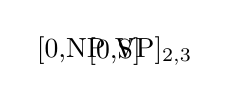
\begin{tikzpicture}
        \Tree
            [.\node(root){[0,\psep S]};
                \node (0) {[0,\psep NP VP]$_{2,3}$};
            ]
    \end{tikzpicture}
\end{center}
%
Note that [0,\psep NP VP] has subscripts $2$ and $3$ to indicate that we can use rules 2 and 3 of our CFG to predict new parse items.
Suppose the parser uses predict(3) to create the item [0,\psep Det N VP].
Then this item is added as a daughter of [0,\psep NP VP] to the previous tree, and the subscript 3 is also removed from [0,\psep NP VP].
We do not need to add a subscript to [0,\psep Det N VP] since it is a leaf.
%
\begin{center}
    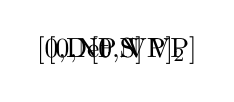
\begin{tikzpicture}
        \Tree
            [.\node(root){[0,\psep S]};
                [.\node(0){[0,\psep NP VP]$_{2}$};
                    \node(00){[0,\psep Det N VP]};
                ]
            ]
    \end{tikzpicture}
\end{center}
%
The next step of the parser now depends on how the control structure prioritizes distinct parses.
We can either expand the table that ends in [0,\psep Det N VP], or go back to the one ending in [0,\psep NP VP] and apply predict(2).
Suppose we do the latter, so that [0,\psep PN VP] is added as the second daughter of [0,\psep NP VP], which thus loses its last subscript.
%
\begin{center}
    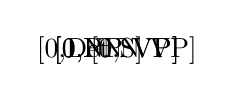
\begin{tikzpicture}
        \Tree
            [.\node(root){[0,\psep S]};
                [.\node(0){[0,\psep NP VP]};
                    \node(00){[0,\psep Det N VP]};
                    \node(01){[0,\psep PN VP]};
                ]
            ]
    \end{tikzpicture}
\end{center}
%
Now let's expand [0,\psep Det N VP] again to obtain [0, \psep the N VP] and then apply a scan step, yielding [1, \psep N VP].
%
\begin{center}
    
\begin{tikzpicture}
        \Tree
            [.\node(root){[0,S]};
                [.\node(0){[0,NP VP]};
                    [.\node(00){[0,Det N VP]};
                        [.\node(000){[0,the N VP]};
                            \node (0000) {[1,N VP]};
                        ]
                    ]
                    \node(01){[0,PN VP]};
                ]
            ]
    \end{tikzpicture}
\end{center}
%
If our parser is really smart, it will be able to infer at this point that the scanned word \emph{the} can never be obtained from [0,PN VP] (technically this is achieved by associating every parse item $p$ with a regular expression that describes the possible left edges of the strings that can be derived from $p$).
So the parser can remove [0,PN VP] from the tree, which is tantamount to discarding the parse table where NP was rewritten as PN\@.
%
\begin{center}
    
\begin{tikzpicture}
        \Tree
            [.\node(root){[0,S]};
                [.\node(0){[0,NP VP]};
                    [.\node(00){[0,Det N VP]};
                        [.\node(000){[0,the N VP]};
                            \node (0000) {[1,N VP]};
                        ]
                    ]
                ]
            ]
    \end{tikzpicture}
\end{center}

\end{examplebox}

What makes the tree representation of the parse space appealing is that the construction and prioritization of parse tables can be reduced to strategies for tree building.
In particular, the familiar notions of depth-first and breadth-first carry over in a natural fashion.
%
\begin{description}
    \item[depth first/serial] expand a parse item $p$ that was introduced during the previous parse step; if the parse item $p$ cannot be expanded, expand the lowest parse leaf $l$ that dominates $p$
    \item[breadth first/parallel] before expanding a parse item introduced during parse step $j$, all parse items that were introduced at parsing step $i$ must have been rewritten, for every $i < j$
\end{description}
%
The depth first strategy leads to a parser that always builds a single complete parse history rather than multiple partial ones.
If the parse history cannot be expanded anymore, the parser either stops (successful parse) or backtracks to the last choice point in the parse history and tries a different choice instead.
This corresponds exactly to the notion of serial parsing in the psycholinguistic literature, and as we saw in example~\ref{ex:TopDownEval_PriorityQueue} this can be implemented as a stack, i.e.\ a priority queue where new parse items are always added at the start of the queue.

The intuitive counterpart of serial parsing is \emph{fully parallel parsing}, where all parse tables are built up at the same time.
This is exactly the behavior of the breadth-first strategy or a priority queue where new parse items are added at the end
However, even proponents of parallel parsing usually do not assume that the human parser computes and stores all options all the time.
Instead, only a subset of very likely parses is claimed to be worked on in parallel, with all others either discarded or at least not expanded on.
On a technical level we may formalize this in terms of a probabilistic procedure for which parse items may be expanded, and in which order.
The details are not important here, the basic insights is simply that just as we can add probabilities to the control schema to regulate which inference rules the parser may apply, we can also use probabilities to prioritize the expansion of certain parse tables over others.

\subsection{Formal Account of Garden Paths}
\label{sub:TopDownEval_FormalGardenPath}
A recursive descent parser with a depth-first expansion strategy for prefix trees, coupled with a preference ranking over prediction steps, can easily account for garden path effects.
In the case of \emph{the horse raced past the barn fell}, for example, the parse builds a single parse table, and due to how certain rewrite rules are preferred over others, this parse table encodes the structure for \emph{the horse raced past the barn}.
When encountering \emph{fell}, the parser has to backtrack.
A successful parse requires backtracking to the point where \emph{raced} is analyzed as part of the VP rather than the NP --- that's quite a distance.
%
\begin{examplebox}[Backtracking in \emph{the horse raced past the barn fell}]
    Assume we have the following (massively simplified) grammar:
    %
    \begin{center}
        \begin{tabular}{rrlp{2em}rrl}
            1)  & S   & \rewrite NP VP
                & & 
            8)  & Det & \rewrite the
            \\
            2)  & NP  & \rewrite Det N
                & &
            9)  & N   & \rewrite barn
            \\
            3)  & NP  & \rewrite Det N VP$_\mathit{rel}$
                & & 
            10) & N   & \rewrite horse 
            \\
            4)  & VP  & \rewrite V
                & & 
            11) & P   & \rewrite past
            \\
            5)  & VP  & \rewrite V PP
                & & 
            12) & V   & \rewrite fell 
            \\
            6)  & VP$_\mathit{rel}$  & \rewrite V$_\mathit{rel}$ PP
                & & 
            13) & V   & \rewrite raced
            \\
            7)  & PP  & \rewrite P NP
                & & 
            14) & V$_\mathit{rel}$   & \rewrite raced
        \end{tabular}
    \end{center}
    %
    Here's the resulting tree for our garden path sentence.
    %
    \begin{center}
        \begin{tikzpicture}
            \Tree
                [.S
                    [.NP
                        [.Det the ]
                        [.N horse ]
                        [.VP$_\mathit{rel}$
                            [.V$_\mathit{rel}$ raced ]
                            [.PP
                                [.P past ]
                                [.NP
                                    [.Det the ]
                                    [.N barn ]
                                ]
                            ]
                        ]
                    ]
                    [.VP
                        [.V fell ]
                    ]
                ]
        \end{tikzpicture}
    \end{center}
    %
    If the parser prefers NP \rewrite\ Det N over NP \rewrite Det N CP and operates in a recursive descent fashion, the construction of the first parse table results in the prefix tree below.
    %
    \begin{center}
        \footnotesize
        \begin{tikzpicture}[level 1+/.style = { level distance = 2em }]
            \Tree
                [.{[0,\psep S]}
                [.{[0,\psep NP VP]$_3$}
                [.{[0,\psep Det N VP]}
                [.{[0, \psep the N VP]}
                [.{[1,\psep N VP]$_9$}
                [.{[1,\psep horse VP]}
                [.{[2,\psep VP]$_4$}
                [.{[2,\psep V PP]$_{12}$}
                [.{[2,\psep raced PP]}
                [.{[3,\psep PP]}
                [.{[3,\psep P NP]}
                [.{[3,\psep past NP]}
                [.{[4,\psep NP]$_3$}
                [.{[4,\psep Det N]}
                [.{[4,\psep the N]}
                [.{[5,\psep N]$_{10}$}
                [.{[5,\psep barn]}
                [.{[6,\psep]}
                ]]]]]]]]]]]]]]]]]]
        \end{tikzpicture}
    \end{center}
    %
    Since this parse does not succeed, the parser needs to backtrack.
    The closest choice point is [5,\psep N]$_{10}$, which obviously does not fix the problem of integrating \emph{fell} into the structure, as can be verified after a single scan step.
    The next choice point is [4,\psep NP]$_3$.
    Here the parser still has the option of replacing NP by Det N CP, which won't help much either, but it takes quite a while to realize this because the tree for the parse table obtained by following this option involves a choice point, too.
    %
    \begin{center}
        \footnotesize
        \begin{tikzpicture}[level 1+/.style = { level distance = 2em }]
            \Tree
                [.{[4,\psep NP]}
                    [.{[4,\psep Det N VP$_\mathit{rel}$]}
                        [.{[4,\psep the N VP$_\mathit{rel}$]}
                            [.{[5,\psep N VP$_\mathit{rel}$]}
                                [.{[5,\psep barn VP$_\mathit{rel}$]}
                                    [.{[6,\psep VP$_\mathit{rel}$]}
                                        [.{[6,\psep V$_\mathit{rel}$ PP]}
                                            {[6,\psep fell PP]}
                                        ]
                                    ]
                                ]
                                {[5,\psep horse VP$_\mathit{rel}$]}
                            ]
                        ]
                    ]
                ]
        \end{tikzpicture}
    \end{center}
    %
    Since this venue didn't yield a successful parse either, the parse backtracks to [2,\psep V PP]$_{12}$, and after this fails, to [2,\psep VP]$_4$.
    Once again it is not successful, and the same holds once it expands [1,\psep N VP].
    %
    \begin{center}
        \footnotesize
        \begin{tikzpicture}[level 1+/.style = { level distance = 2em }]
            \Tree
                [.{[2,\psep V PP]}
                    {[2,\psep fell PP]}
                ]

            \begin{scope}[xshift=8em]
                \Tree
                    [.{[2,\psep VP]}
                        [.{[2,\psep V]}
                            {[2,\psep fell]}
                            {[2,\psep raced]}
                        ]
                    ]
            \end{scope}

            \begin{scope}[xshift=16em]
                \Tree
                    [.{[1,\psep N VP]}
                        {[1,\psep barn VP]}
                    ]
            \end{scope}
        \end{tikzpicture}
    \end{center}
    %
    Only if the parser backtracks all the way to [0,\psep NP VP]$_3$, essentially undoing all its work so far, can it find a working parse.
    %
    \begin{center}
        \footnotesize
        \begin{tikzpicture}[level 1+/.style = { level distance = 2em}]
            \Tree
                [.{[0,\psep NP VP]}
                    [.{[0,\psep Det N VP$_\mathit{rel}$ VP]}
                        [.{[0,\psep the N VP$_\mathit{rel}$ VP]}
                            [.{[1,\psep N VP$_\mathit{rel}$ VP]}
                                {[1,\psep barn VP$_\mathit{rel}$ VP]}
                                [.{[1,\psep horse VP$_\mathit{rel}$ VP]}
                                    [.{[2,\psep VP$_\mathit{rel}$ VP]}
                                        [.{[2,\psep V$_\mathit{rel}$ PP VP]}
                                            [.{[3,\psep raced PP VP]}
                                                [.{[4,\psep PP VP]}
                                                    [.{[4,\psep P NP VP]}
                                                        [.{[4,\psep past NP VP]}
                                                            [.{[5,\psep NP VP]}
                                                                [.{[5,\psep Det N VP]}
                                                                    [.{[5,\psep the N VP]}
                                                                        [.{[6,\psep N VP]$_{10}$}
                                                                            [.{[6,\psep barn VP]}
                                                                                [.{[7,\psep VP]}
                                                                                    [.{[7,\psep V]$_{13}$}
                                                                                        [.{[7,\psep fell]}
                                                                                            {[7,\psep]}
                                                                                        ]
                                                                                    ]
                                                                                ]
                                                                            ]
                                                                        ]
                                                                    ]
                                                                ]
                                                            ]
                                                        ]
                                                    ]
                                                ]
                                            ]
                                        ]
                                    ]
                                ]
                            ]
                        ]
                    ]
                ]
        \end{tikzpicture}
    \end{center}
    %
    The prefix tree for all the parse histories built by the parser before it encounters a successful parse it much bigger than the simple phrase structure tree for the sentence.
    %
    \begin{center}
        \footnotesize
        \label{fig:TopDownEval_ParseHistory}
        \begin{tikzpicture}[%
            level 1+/.style = { level distance = 2em },
            level 5/.style = { sibling distance= -5em },
            level 7/.style = { sibling distance= -5em },
            level 8/.style = { sibling distance= -10em }
            ]
            \Tree
                [.{[0,\psep S]}
                    [.{[0,\psep NP VP]}
                        [.{[0,\psep Det N VP]}
                            [.{[0, \psep the N VP]}
                                [.{[1,\psep N VP]}
                                    [.{[1,\psep horse VP]}
                                        [.{[2,\psep VP]}
                                            [.{[2,\psep V PP]}
                                                [.{[2,\psep raced PP]}
                                                    [.{[3,\psep PP]}
                                                        [.{[3,\psep P NP]}
                                                            [.{[3,\psep past NP]}
                                                                [.{[4,\psep NP]}
                                                                    [.{[4,\psep Det N]}
                                                                        [.{[4,\psep the N]}
                                                                            [.{[5,\psep N]}
                                                                                [.{[5,\psep barn]}
                                                                                    {[6,\psep]}
                                                                                ]
                                                                                {[5,\psep horse]}
                                                                            ]
                                                                        ]
                                                                    ]
                                                                    [.{[4,\psep Det N VP$_\mathit{rel}$]}
                                                                        [.{[4,\psep the N VP$_\mathit{rel}$]}
                                                                            [.{[5,\psep N VP$_\mathit{rel}$]}
                                                                                [.{[5,\psep barn VP$_\mathit{rel}$]}
                                                                                    [.{[6,\psep VP$_\mathit{rel}$]}
                                                                                        [.{[6,\psep V$_\mathit{rel}$ PP]}
                                                                                            {[6,\psep fell PP]}
                                                                                        ]
                                                                                    ]
                                                                                ]
                                                                                {[5,\psep horse VP$_\mathit{rel}$]}
                                                                            ]
                                                                        ]
                                                                    ]
                                                                ]
                                                            ]
                                                        ]
                                                    ]
                                                ]
                                                {[2,\psep fell PP]}
                                            ]
                                            [.{[2,\psep V]}
                                                {[2,\psep raced]}
                                                {[2,\psep fell]}
                                            ]
                                        ]
                                    ]
                                {[1,\psep barn VP]}
                                ]
                            ]
                        ]
                        [.{[0,\psep Det N VP$_\mathit{rel}$ VP]}
                            [.{[0,\psep the N VP$_\mathit{rel}$ VP]}
                                [.{[1,\psep N VP$_\mathit{rel}$ VP]}
                                    {[1,\psep barn VP$_\mathit{rel}$ VP]}
                                    [.{[1,\psep horse VP$_\mathit{rel}$ VP]}
                                        [.{[2,\psep VP$_\mathit{rel}$ VP]}
                                            [.{[2,\psep V$_\mathit{rel}$ PP VP]}
                                                [.{[3,\psep raced PP VP]}
                                                    [.{[4,\psep PP VP]}
                                                        [.{[4,\psep P NP VP]}
                                                            [.{[4,\psep past NP VP]}
                                                                [.{[5,\psep NP VP]}
                                                                    [.{[5,\psep Det N VP]}
                                                                        [.{[5,\psep the N VP]}
                                                                            [.{[6,\psep N VP]$_{10}$}
                                                                                [.{[6,\psep barn VP]}
                                                                                    [.{[7,\psep VP]}
                                                                                        [.{[7,\psep V]$_{13}$}
                                                                                            [.{[7,\psep fell]}
                                                                                                {[7,\psep]}
                                                                                            ]
                                                                                        ]
                                                                                    ]
                                                                                ]
                                                                            ]
                                                                        ]
                                                                    ]
                                                                ]
                                                            ]
                                                        ]
                                                    ]
                                                ]
                                            ]
                                        ]
                                    ]
                                ]
                            ]
                        ]
                    ]
                ]
        \end{tikzpicture}
    \end{center}
\end{examplebox}

In sum, the Frazier model can be defined more rigorously as a recursive descent parser with a stack as its priority queue.
As the Frazier model is designed to account for garden paths, it is no surprise that its formal counterparts makes the right processing predictions in this case.

\section{Center Embedding}
\label{sub:TopDownEval_CenterEmbedding}
It is a well-known fact that center embedding constructions are harder to parse than right embedding constructions, even if one controls for sentence length, discourse and vocabulary.
%
\begin{exe}
    \ex
    \begin{xlist}
        \ex I bought the cheese (that) the mouse (that) the cat (that) the dog chased ate wanted.
        \ex I bought the cheese (that) the mouse wanted (that) the cat ate (that) the dog wanted.
    \end{xlist}
\end{exe}
%
A common idea is that the difficulty of center embedding has to do with an increased memory burden, either because more items have to be kept in memory for a non-trivial amount of time, or because specific items have to be stored for a longer time, or a combination of the two.
The specifics vary between accounts.

\citet{Kimball73}, for instance, proposes that the parser cannot work on more than two sentences at once, i.e.\ it is possible to keep up to two CPs in memory, but not more than that.
Right embedding of CPs is fine because opening a new CP is the last step needed to close the containing CP, which can subsequently be removed from memory.
Center embedding, on the other hand, requires that both CPs be stored in memory, so it is limited to one level of embedding.

\posscitet{Gibson98} \emph{Syntactic Prediction Locality Theory} (SPLT) contends that memory burden increases the more dependencies need to be stored at the same time, and since center embedding of the type NP-S-VP necessarily involves starting a new dependency before the old one between NP and VP has been finished, center embedding is difficult.

This argument can be ported into our more formal setting via a \emph{linking hypothesis} between control structure and processing difficulty.
Remember that we can annotate phrase structure trees to indicate the order in which nodes are introduced and rewritten by the parser.
Obviously any item that is not rewritten immediately after its introduction --- i.e.\ any item whose prefix and suffix differ by more than 1 --- needs to be stored in memory.
Let's put these items in boxes so that they are easy to pick out at a glance.
Parsing difficulty, then, can be measured in a variety of ways.
%
\begin{description}
    \item[Tenure] the \emph{tenure of node $n$} is the difference between its subscript and its superscript
    \item[Payload] the \emph{payload of tree $t$} is the number of nodes whose tenure is strictly greater than $1$
\end{description}
%
These two measures can be combined to create a variety of difficulty metrics such as the two below (cf.\ \citealt{Kobele.etal12}, \citealt{GrafMarcinek14CMCL}, and \citealt{GrafEtAl15MOL}).
%
\begin{description}
    \item[MaxTen] greatest tenure among all the nodes; $\max(\setof{ \mathrm{tenure}(n) })$
    \item[SumTen] total number of steps that items must be memorized; $\sum(\setof{ \mathrm{tenure}(n) > 1})$
\end{description}
%
All of these metrics capture the fact that right embedding isn't harder than center embedding.
\textbf{MaxTen} and \textbf{SumTen} also predict right embedding to be easier.

\begin{examplebox}[Center embedding and maximum tenure]
    Consider the center embedding and right embedding trees below, which have been annotated according to the behavior of a recursive descent parser.
    For center embedding we are using a promotion-style analysis of relative clauses \citep{Vergnaud74, Kayne94}, which posits that the relative clause is an argument of the determiner, with the head noun residing in a CP specifier.
    For right embedding the extraposed relative clause is considered a daughter of S.
    %
    \begin{center}
        \footnotesize
        \begin{tikzpicture}[
            level 1+/.style = { level distance = 2.5em },
            level 2/.style = { sibling distance = -.75em },
            level 3/.style = { sibling distance = -1em },
            level 4/.style = { sibling distance = -1em },
            level 5/.style = { sibling distance = -2.5em }
            ]
            \Tree
                [.\Lab{S}{1}{2}
                    [.\Lab{NP}{2}{3}
                        [.\Lab{N}{3}{4}
                            \Lab{I}{4}{5}
                        ]
                    ]
                    [.\IBLab{VP}{2}{6}
                        [.\Lab{V}{6}{7}
                            \Lab{bought}{7}{8}
                        ]
                        [.\IBLab{NP}{6}{9}
                            [.\Lab{Det}{9}{10}
                                \Lab{the}{10}{11}
                            ]
                            [.\IBLab{CP}{9}{12}
                                [.\Lab{N}{12}{13}
                                    \Lab{cheese}{13}{14}
                                ]
                                [.\IBLab{C}{12}{15}
                                    \Lab{that}{15}{16}
                                ]
                                [.\IBLab{S}{12}{17}
                                    [.\Lab{NP}{17}{18}
                                        [.\Lab{Det}{18}{19}
                                            \Lab{the}{19}{20}
                                        ]
                                        [.\IBLab{CP}{18}{21}
                                            [.\Lab{N}{21}{22}
                                                \Lab{mouse}{22}{23}
                                            ]
                                            [.\IBLab{C}{21}{24}
                                                \Lab{that}{24}{25}
                                            ]
                                            [.\IBLab{S}{21}{26}
                                                [.\Lab{NP}{26}{27}
                                                    [.\Lab{Det}{27}{28}
                                                        \Lab{the}{28}{29}
                                                    ]
                                                    [.\IBLab{N}{27}{30}
                                                        \Lab{cat}{30}{31}
                                                    ]
                                                ]
                                                [.\IBLab{VP}{26}{32}
                                                    [.\Lab{V}{32}{33}
                                                        \Lab{ate}{33}{34}
                                                    ]
                                                ]
                                            ]
                                        ]
                                    ]
                                    [.\IBLab{VP}{17}{35}
                                        [.\Lab{V}{35}{36}
                                            \Lab{wanted}{36}{37}
                                        ]
                                    ]
                                ]
                            ]
                        ]
                    ]
                ]
        \end{tikzpicture}

        \begin{tikzpicture}[
            level 1+/.style = { level distance = 2.5em },
            level 2/.style = { sibling distance = -.75em },
            level 3/.style = { sibling distance = -1em },
            level 4/.style = { sibling distance = -1em },
            level 5/.style = { sibling distance = -1em },
            level 6/.style = { sibling distance = -1em }
            ]
            \Tree
                [.\Lab{S}{1}{2}
                    [.\Lab{NP}{2}{3}
                        [.\Lab{N}{3}{4}
                            \Lab{I}{4}{5}
                        ]
                    ]
                    [.\IBLab{VP}{2}{6}
                        [.\Lab{V}{6}{7}
                            \Lab{bought}{7}{8}
                        ]
                        [.\IBLab{NP}{6}{9}
                            [.\Lab{Det}{9}{10}
                                \Lab{the}{10}{11}
                            ]
                            [.\IBLab{CP}{9}{12}
                                [.\Lab{N}{12}{13}
                                    \Lab{cheese}{13}{14}
                                ]
                                [.\IBLab{C}{12}{15}
                                    \Lab{that}{15}{16}
                                ]
                                [.\IBLab{S}{12}{17}
                                    [.\Lab{NP}{17}{18}
                                        [.\Lab{Det}{18}{19}
                                            \Lab{the}{19}{20}
                                        ]
                                        [.\IBLab{N}{18}{21}
                                            \Lab{mouse}{21}{22}
                                        ]
                                    ]
                                    [.\IBLab{VP}{17}{23}
                                        [.\Lab{V}{23}{24}
                                            \Lab{wanted}{24}{25}
                                        ]
                                    ]
                                    [.\IBLab{CP}{17}{26}
                                        [.\Lab{C}{26}{27}
                                            \Lab{that}{27}{28}
                                        ]
                                        [.\IBLab{S}{26}{29}
                                            [.\Lab{NP}{29}{30}
                                                [.\Lab{Det}{30}{31}
                                                    \Lab{the}{31}{32}
                                                ]
                                                [.\IBLab{N}{30}{33}
                                                    \Lab{cat}{33}{34}
                                                ]
                                            ]
                                            [.\IBLab{VP}{29}{35}
                                                [.\Lab{V}{35}{36}
                                                    \Lab{ate}{36}{37}
                                                ]
                                            ]
                                        ]
                                    ]
                                ]
                            ]
                        ]
                    ]
                ]
        \end{tikzpicture}
    \end{center}
    %
    The difficult center embedding sentence has a payload of 11, a maximum tenure of 17, and a sum tenure of 55.
    The easier right embedding sentence has a payload of 11, a maximum tenure of 9, and a sum tenure of 48.
    Irrespective of how we weigh or rank these three metrics, then, right embedding is never predicted to be harder than center embedding.
    As long as we do not take payload as the only difficulty metric, right embedding is correctly predicted to be easier than center embedding.
\end{examplebox}

Notice that our explanation for the difficulty of center embedding is very different from the one we used for garden path effects.
Garden path effects were explained in terms of the difficulty of finding a right parse among the many possible ones.
We used prefix trees as a way of representing the parser's route through this search space, and since a prefix tree encodes many parsing tables at ones, our account is ultimately based on the processing challenges of coordinating multiple parse tables --- if all parse tables could be easily stored in memory and expanded in a breadth-first manner, garden path effects would not arise.

Center embedding, on the other hand, is explained purely in terms of how the parser constructs the correct parse.
How the parser actually finds this parse does not factor into the explanation.
The claim is that even if the parser had a perfect \emph{oracle}, a machine that could tell it at every step which inference step must be taken to get the correct structure, the difference between center embedding and right embedding would not disappear because the former still puts a higher load on working memory than the latter.

\section{Problems}
\label{sec:TopDownEval_Problems}

\subsection{Memory Usage in Left Embedding}
\label{sub:TopDownEval_LeftEmbedding}
A careful examination of the top-down parsers behavior over center embedding constructions reveals that these configurations aren't the only ones that should cause an increased memory burden.
Coupled with our metrics of processing difficulty, a recursive descent parser predicts that left embedding should be hard to parse, too --- which is not borne out empirically.
%
\begin{exe}
    \ex
    \begin{xlist}
        \ex The exhaust pipe of the car of the father of the mechanic is broken.
        \ex The mechanic's father's car's exhaust pipe is broken.
    \end{xlist}
\end{exe}
%
The cause for the predicted difficulty spike with left embedding is straight-forward.
Suppose the parser conjectures at step $i$ that node $n$ in the tree has daughters $d_1$ and $d_2$.
Steps $i+1$ to $j$ are spent by the parser expanding the subtree rooted in $d_1$.
The bigger the subtree, the higher the value of $j + 1$, the point at which the parser can move on to expanding $d_2$.
Since $d_2$ must be kept in memory from step $i$ until step $j + 1$, and the value of $j$ increases with the size of the subtree rooted in $d_1$, every construction that increases the size of a left sibling --- including left embedding --- should increase parsing difficulty.

\subsection{Looping in Left Recursion}
\label{sub:TopDownEval_LeftRecursion}

Left embedding constructions are problematic for top-down parsers in more respects than just psycholinguistic adequacy.
Consider a grammar that licenses possessive structures such as the one below.
%
\begin{center}
    \begin{tikzpicture}
        \Tree
            [.S
                [.NP
                    [.NP
                        [.NP
                            [.N John ]
                        ]
                        [.Poss 's ]
                        [.N father ]
                    ]
                    [.Poss 's ]
                    [.N car ]
                ]
                [.VP
                    [.V disappeared ]
                ]
            ]
    \end{tikzpicture}
\end{center}
%
In order to arrive at this structure, the parser must first infer [0,\psep NP VP], and then expand the NP to get [0,\psep NP Poss N VP].
But now the parser once again has to expand the NP, possibly creating [0,\psep NP Poss N Poss N VP].
It is easy to see that the parser can keep rewriting NP \emph{ad infinitum}, essentially looping the NP rewriting step and producing longer and longer parse items.
Without a smart control structure that detects this kind of looping, the parser will soon run out of working memory, or if there is no limit on the amount of memory, keep looping forever without ever constructing a parse.

A standard solution is to use a probabilistic control structure that prunes away all parse tables that fall below a certain probability threshold.
As the parser keeps conjecturing bigger and bigger structures, the probability of these parses decreases until they are eventually pruned away.
This is also called a \emph{beam parser}.
Beam parsers require a method for automatically inferring the necessary probabilities from a corpus, and their overall behavior can be difficult to figure out.
So the appealing simplicity of top-down parsers is lost to some extent.
For more details on top-down beam parsing, see \citet{Roark01a, Roark01b, Roark04}.

\subsection{Merely Local Syntactic Coherence Effects}
\label{sub:TopDownEval_CoherenceEffects}
Merely local syntactic coherence effects is a term coined by \citet{Tabor.etal04} to refer to cases where an analysis that is locally well-formed but incompatible with the structure built so far nonetheless induces a temporary increase in parsing difficulty (see also \citealt{Konieczny05}, \citealt{Konieczny.etal09}, and \citealt{Bicknell.etal09}).
This is exemplified by the contrast in \eqref{ex:TopDownEval_LocalCoherence}.
During self-paced reading experiments, subjects' reading speed of \eqref{ex:TopDownEval_LocalCoherenceObserved} decreases at \emph{tossed}, indicating an increase in processing difficulty.
The effect disappears, however, when \emph{tossed} is replaced by \emph{thrown}.
%
\begin{exe}
    \ex\label{ex:TopDownEval_LocalCoherence}
    \begin{xlist}
        \ex The coach smiled at the player tossed a frisbee.\label{ex:TopDownEval_LocalCoherenceObserved}
        \ex The coach smiled at the player thrown a frisbee.\label{ex:TopDownEval_LocalCoherenceNotObserved}
    \end{xlist}
\end{exe}
%
It seems as if the fact that \emph{the player} can be locally analyzed as the subject of \emph{tossed} confuses the parser. 
Since this interpretation is not available with \emph{thrown} due to the unambiguous past participle morphology, no slowdown occurs.

Merely local syntactic coherence effects are completely unexpected with a top-down parser because there is no way the parser could infer an item that treats \emph{tossed} as a finite verb with \emph{the player} as its subject.
The preceding parts of the sentence have already disambiguated the structure of the sentence to an extent where this is no longer a viable hypothesis.
These effects are expected, however, if the parser proceeds bottom-up instead of top-down.
More on that in chapter~\ref{cha:BottomUp}.

\bibliographystyle{../../linquiry3}
\bibliography{../../universal,../../graf}

\chapter{Bottom-Up Parsing}
\label{cha:BottomUp}

The natural counterpart to top-down parsing is bottom-up parsing, where trees are built starting at the leaves and moving towards the root.
Like top-down parsing, bottom-up parsing is fairly simple and acts as the foundation of a variety of parsing algorithms.
But just like top-down parsing, it has certain shortcomings regarding psycholinguistic adequacy.

\section{Intuition}
\label{sec:BottomUp_Intuition}
For illustration we use the same grammar as for the top-down parser in Lecture~\ref{cha:TopDown}.
%
\begin{center}
    \begin{tabular}{rrcl@{\hspace{2em}}rrcl}
        1)  & S   & \rewrite\ & NP VP
        &
        6)  & Det & \rewrite\ & a | the
        \\
        2)  & NP  & \rewrite\ & PN
        &
        7)  & N   & \rewrite\ & car | truck | anvil
        \\
        3)  & NP  & \rewrite\ & Det
        &
        8)  & PN  & \rewrite\ & Bugs | Daffy
        \\
        4)  & VP  & \rewrite\ & Vi
        &
        9)  & Vi  & \rewrite\ & fell over
        \\
        5)  & VP  & \rewrite\ & Vt NP
        &
        10) & Vt  & \rewrite\ & hit
        \\
    \end{tabular}
\end{center}
%
A bottom-up parser essentially applies the rewrite rules in reverse.
If the current input $i$ appears on the right-hand side of a rewrite rule for $N$, replace $i$ by $N$.
%
\begin{center}
    \begin{tabular}{r|l}
        \textbf{string} & \textbf{rule}\\
        the & read input\\
        det & Det \rewrite the\\
        det anvil & read input\\
        det N & N \rewrite anvil\\
        NP & NP \rewrite Det N\\
        NP hit & read input\\
        NP Vt & Vt \rewrite hit\\
        NP Vt Daffy & read input\\
        NP Vt PN & PN \rewrite Daffy\\
        NP Vt NP & NP \rewrite PN\\
        NP VP & VP \rewrite Vt NP\\
        S & S \rewrite NP VP
    \end{tabular}
\end{center}

The order in which rules are applied once again gives rise to at least four different types of parsers, a helpful first approximation of which can be gleaned from the examples below.
The four trees below correspond to (in clockwise order) left-to-right depth first, right-to-left depth first, right-to-left breadth first, and left-to-right breadth first.
%
\begin{center}
    \begin{tikzpicture}
        \Tree
            [.\Lab{S}{12}{}
                [.\Lab{NP}{5}{12}
                    [.\Lab{Det}{2}{5}
                        \Lab{the}{1}{2}
                    ]
                    [.\Lab{N}{4}{5}
                        \Lab{anvil}{3}{4}
                    ]
                ]
                [.\Lab{VP}{11}{12}
                    [.\Lab{Vt}{7}{11}
                        \Lab{hit}{6}{7}
                    ]
                    [.\Lab{NP}{10}{11}
                        [.\Lab{PN}{9}{10}
                            \Lab{Daffy}{8}{9}
                        ]
                    ]
                ]
            ]
    \end{tikzpicture}
    %
    \begin{tikzpicture}
        \Tree
            [.\Lab{S}{12}{}
                [.\Lab{NP}{11}{12}
                    [.\Lab{Det}{10}{11}
                        \Lab{the}{9}{10}
                    ]
                    [.\Lab{N}{8}{11}
                        \Lab{anvil}{7}{8}
                    ]
                ]
                [.\Lab{VP}{6}{12}
                    [.\Lab{Vt}{5}{6}
                        \Lab{hit}{4}{5}
                    ]
                    [.\Lab{NP}{3}{6}
                        [.\Lab{PN}{2}{3}
                            \Lab{Daffy}{1}{2}
                        ]
                    ]
                ]
            ]
    \end{tikzpicture}

    \begin{tikzpicture}
        \Tree
            [.\Lab{S}{12}{}
                [.\Lab{NP}{9}{12}
                    [.\Lab{Det}{5}{9}
                        \Lab{the}{1}{5}
                    ]
                    [.\Lab{N}{6}{9}
                        \Lab{anvil}{2}{6}
                    ]
                ]
                [.\Lab{VP}{11}{12}
                    [.\Lab{Vt}{7}{11}
                        \Lab{hit}{3}{7}
                    ]
                    [.\Lab{NP}{10}{11}
                        [.\Lab{PN}{8}{10}
                            \Lab{Daffy}{4}{8}
                        ]
                    ]
                ]
            ]
    \end{tikzpicture}
    %
    \hspace{1em}
    %
    \begin{tikzpicture}
        \Tree
            [.\Lab{S}{12}{}
                [.\Lab{NP}{11}{12}
                    [.\Lab{Det}{8}{11}
                        \Lab{the}{4}{8}
                    ]
                    [.\Lab{N}{7}{11}
                        \Lab{anvil}{3}{7}
                    ]
                ]
                [.\Lab{VP}{10}{12}
                    [.\Lab{Vt}{6}{10}
                        \Lab{hit}{2}{6}
                    ]
                    [.\Lab{NP}{9}{10}
                        [.\Lab{PN}{5}{9}
                            \Lab{Daffy}{1}{5}
                        ]
                    ]
                ]
            ]
    \end{tikzpicture}
\end{center}


\section{Formal Specification}
\label{sec:BottomUp_Formal}

\subsection{Parsing Schema}
\label{sub:BottomUp_Schema}

Since bottom-up parsers are essentially the dual of top-down parsers, the former's deductive definition closely resembles that of the latter.
Whereas a top-down parser starts with $[0,S,n]$ and seeks to derive $[n,,n]$, the bottom-up parser has axiom $[0,,0]$ and goal $[0,S,n]$.
So axioms and goals are simply switched (and $[n,,n]$ is replaced by $[0,,0]$).
Similarly, the top-down scan and predict rules have bottom-up counterparts Shift and Reduce.
The reduce rule is exactly the predict rule of a top-down parser with top and bottom switched.
The shift rule is the scan rule of a right-to-left top-down parser with top and bottom switched. 

\begin{prooftree}
    \AxiomC{$[i, \beta, j]$}
    \LeftLabel{\textbf{Shift}\qquad}
    \RightLabel{$a = w_{j}$}
    \UnaryInfC{$[i, \beta a,j+1]$}
\end{prooftree}

\begin{prooftree}
    \AxiomC{$[i, \alpha \gamma \beta, j]$}
    \LeftLabel{\textbf{Reduce}\qquad}
    \RightLabel{$N \rewrite \gamma \in R$}
    \UnaryInfC{$[i, \alpha N \beta, j]$}
\end{prooftree}

\begin{examplebox}[Bottom-up parse of \emph{The anvil hit Daffy}]
    Here's a bottom-up parse table for our standard example sentence \emph{The anvil hit Daffy} using the parsing schema above.
    Note that rules are applied in arbitrary order to reflect the fact that the parsing schema still lacks a control structure and thus imposes no specific rule order.
    %
    \begin{center}
        \begin{tabular}{r|l}
            \textbf{parse item} & \textbf{inference rule}\\
            $\lbrack$0,,0] & axiom\\
            $\lbrack$0,the,1] & shift\\
            $\lbrack$0,the anvil,2] & shift\\
            $\lbrack$0,the N,2] & reduce(7)\\
            $\lbrack$0,Det N,2] & reduce(6)\\
            $\lbrack$0,Det N hit,3] & shift\\
            $\lbrack$0,NP hit,3] & reduce(3)\\
            $\lbrack$0,NP hit Daffy,4] & shift\\
            $\lbrack$0,NP hit PN,4] & reduce(8)\\
            $\lbrack$0,NP Vt PN,4] & reduce(10)\\
            $\lbrack$0,NP Vt NP,4] & reduce(2)\\
            $\lbrack$0,NP VP,4] & reduce(5)\\
            $\lbrack$0,S,4] & reduce(1)
        \end{tabular}
    \end{center}
\end{examplebox}

\subsection{Control Structure}
\label{sub:BottomUp_Control}

The control structure can be (partially) encoded by adding the familiar \psep\ to the rules.

\paragraph{Left-to-right, depth-first}
The only axiom is $[0, \psep ,0]$, and the only goal is $[0,S \psep ,n]$.

\begin{prooftree}
    \AxiomC{$[i, \beta \psep, j]$}
    \LeftLabel{\textbf{Shift}\qquad}
    \RightLabel{$a = w_j$}
    \UnaryInfC{$[i, \beta a \psep, j+1]$}
\end{prooftree}

\begin{prooftree}
    \AxiomC{$[i, \alpha \gamma \psep, j]$}
    \LeftLabel{\textbf{Reduce}\qquad}
    \RightLabel{$N \rewrite \gamma \in R$}
    \UnaryInfC{$[i, \alpha N \psep, j]$}
\end{prooftree}

This kind of parser is also called a \emph{shift reduce parser}.
Notice that even though the parser reads the input from left-to-right, the structure building process is partially right-to-left since the reduction rule reduces elements to the left of \psep\ from right to left.

\paragraph{Left-to-right, breadth first}
It is surprisingly difficult to specifier a breadth first bottom-up parser in a deductive fashion (more on that below), and consequently the rules are a lot more complicated.
The axioms and goals are the same as for the depth-first parser, though.

\begin{prooftree}
    \AxiomC{$[i, \beta \psep, j]$}
    \LeftLabel{\textbf{Shift}\qquad}
    \RightLabel{$a = w_j$}
    \UnaryInfC{$[i, \beta a \psep, j+1]$}
\end{prooftree}

\begin{prooftree}
    \AxiomC{$[i, \alpha \psep \beta \gamma \delta, j]$}
    \LeftLabel{\textbf{Reduce}\qquad}
    \RightLabel{$N \rewrite \gamma \in R$}
    \UnaryInfC{$[i, \alpha \beta N \psep \delta, j]$}
\end{prooftree}

\begin{prooftree}
    \AxiomC{$[i,\alpha \psep \beta, j]$}
    \LeftLabel{\textbf{Return}\qquad}
    \RightLabel{$\alpha \in (N \cup T)^+$, $\neg \exists N [N \rewrite \beta \in R]$}
    \UnaryInfC{$[i, \psep \alpha \beta, j]$}
\end{prooftree}


\begin{examplebox}[Depth-first parse of \emph{The anvil hit Daffy}]
    \phantom{a}
    \begin{center}
        \begin{tabular}{r|l}
            \textbf{parse item} & \textbf{inference rule}\\
            $\lbrack$0,\psep,0]             & axiom\\
            $\lbrack$0,the \psep,1]         & shift\\
            $\lbrack$0,Det \psep,1]         & reduce(6)\\
            $\lbrack$0,Det anvil \psep,2]   & shift\\
            $\lbrack$0,Det N \psep,2]       & reduce(7)\\
            $\lbrack$0,NP \psep,2]          & reduce(3)\\
            $\lbrack$0,NP hit \psep,3]      & shift\\
            $\lbrack$0,NP Vt \psep,3]       & reduce(10)\\
            $\lbrack$0,NP Vt Daffy \psep,4] & shift\\
            $\lbrack$0,NP Vt PN \psep,4]    & reduce(8)\\
            $\lbrack$0,NP Vt NP \psep,4]    & reduce(2)\\
            $\lbrack$0,NP VP \psep,4]       & reduce(5)\\
            $\lbrack$0,S \psep,4]           & reduce(1)
        \end{tabular}
    \end{center}
\end{examplebox}
%
\begin{examplebox}[Breadth-first parse of \emph{The anvil hit Daffy}]
    \phantom{a}
    \begin{center}
        \begin{tabular}{r|l}
            \textbf{parse item}                     & \textbf{inference rule}\\
            $\lbrack$0,\psep,0]                     & axiom\\
            $\lbrack$0,the \psep,1]                 & shift\\
            $\lbrack$0,the anvil \psep,2]           & shift\\
            $\lbrack$0,the anvil hit \psep,3]       & shift\\
            $\lbrack$0,the anvil hit Daffy \psep,4] & shift\\
            $\lbrack$0,\psep the anvil hit Daffy,4] & return\\
            $\lbrack$0,Det \psep anvil hit Daffy,4] & reduce(6)\\
            $\lbrack$0,Det N \psep hit Daffy,4]     & reduce(7)\\
            $\lbrack$0,Det N Vt \psep Daffy,4]      & reduce(10)\\
            $\lbrack$0,Det N Vt PN \psep,4]         & reduce(8)\\
            $\lbrack$0,\psep Det N Vt PN,4]         & return\\
            $\lbrack$0,NP \psep Vt PN,4]            & reduce(3)\\
            $\lbrack$0,NP Vt NP \psep,4]            & reduce(2)\\
            $\lbrack$0,\psep NP Vt NP,4]            & return\\
            $\lbrack$0,NP VP \psep,4]               & reduce(5)\\
            $\lbrack$0,\psep NP VP,4]               & return\\
            $\lbrack$0,S \psep,4]                   & reduce(1)\\
        \end{tabular}
    \end{center}
\end{examplebox}
%
\begin{exercise}
    Mirroring the redundancy of the index $j$ for top-down parsers, index $i$ can safely be eliminated from the parse items of a bottom-up parser.    
    Explain why.
\end{exercise}

\begin{exercise}
    Our breadth-first parser is actually too permissive.
    Show that the rules as given can also be used to construct a depth-first parse of \emph{The anvil hit Daffy}.
\end{exercise}
%
\begin{exercise}
    Is there a way to restrict the breadth-first parser so that it can no longer construct depth-first parses?
\end{exercise}

Notice that both parser have a certain overlap between the rules.
In the case of the depth-first parser, the domains of the shift and reduce rules are not disjoint.
That is to say, for some parse items both shift and reduce are valid continuations of the parse, which is called a \emph{shift reduce conflict}.
Shift reduce conflicts are an unavoidable consequence of non-determinism in the grammar.
A top-down parser faces non-determinism with respect to which rewrite rule to apply to a given non-terminal $N$.
For a bottom-up parser, this step is usually deterministic because distinct non-terminals can be assumed to also have distinct right-hand sides in rewrite rules (rules assigning parts of speech to words are one notable exception).
But the bottom-up parser must decide whether to reduce right away or read another input symbol first, which might allow for a different reduction step.
%
\begin{examplebox}[A depth-first parse with delayed shift]
    Consider the grammar below, which generates conjunctions and disjunctions of proper names.
    %
    \begin{center}
        \begin{tabular}{rrcl}
            1) & NP & \rewrite & NP and NP\\
            2) & NP & \rewrite & NP or NP\\
            3) & NP & \rewrite & John | Mary | Sue
        \end{tabular}
    \end{center}
    %
    Now consider the phrase \emph{John and Mary or Sue}, which has two semantically distinct structures.
    %
    \begin{center}
        \begin{tikzpicture}
            \Tree
                [.NP
                    [.NP
                        [.NP
                            John
                        ]
                        and
                        [.NP
                            Mary
                        ]
                    ]
                    or
                    [.NP Sue ]
                ]
        \end{tikzpicture}
        %
        \hspace{1em}
        %
        \begin{tikzpicture}
            \Tree
                [.NP
                    [.NP
                        John
                    ]
                    and
                    [.NP
                        [.NP
                            Mary
                        ]
                        or
                        [.NP
                            Sue
                        ]
                    ]
                ]
        \end{tikzpicture}
    \end{center}
    %
    If the bottom-up parser reduces as early as possible, we get the tree to the left.
    This also shows that reduction proceeds from the right edge of the parse item.
    %
    \begin{center}
        \begin{tabular}{r|l}
            \textbf{parse item}             & \textbf{inference rule}\\
            $\lbrack$0,\psep,0]             & axiom\\
            $\lbrack$0,John \psep,1]        & shift\\
            $\lbrack$0,NP \psep,1]          & reduce(3)\\
            $\lbrack$0,NP and \psep,2]      & shift\\
            $\lbrack$0,NP and Mary \psep,3] & shift\\
            $\lbrack$0,NP and NP \psep,3]   & reduce(3)\\
            $\lbrack$0,NP \psep,3]          & reduce(1)\\
            $\lbrack$0,NP or \psep,4]       & shift\\
            $\lbrack$0,NP or Sue \psep,5]   & shift\\
            $\lbrack$0,NP or NP \psep,5]    & reduce(3)\\
            $\lbrack$0,NP \psep,5]          & reduce(2)
        \end{tabular}
    \end{center}
    %
    In order to obtain the other tree, the parser must delay the application of reduce(1) until reduce(2).
    %
    \begin{center}
        \begin{tabular}{r|l}
            \textbf{parse item}                  & \textbf{inference rule}\\
            $\lbrack$0,\psep,0]                  & axiom\\
            $\lbrack$0,John \psep,1]             & shift\\
            $\lbrack$0,NP \psep,1]               & reduce(3)\\
            $\lbrack$0,NP and \psep,2]           & shift\\
            $\lbrack$0,NP and Mary \psep,3]      & shift\\
            $\lbrack$0,NP and NP \psep,3]        & reduce(3)\\
            $\lbrack$0,NP and NP or \psep,4]     & shift\\
            $\lbrack$0,NP and NP or Sue \psep,5] & shift\\
            $\lbrack$0,NP and NP or NP \psep,5]  & reduce(3)\\
            $\lbrack$0,NP and NP \psep,5]        & reduce(2)\\
            $\lbrack$0,NP \psep,5]               & reduce(1)
        \end{tabular}
    \end{center}
\end{examplebox}

The breadth-first parser has a comparable overlap between shift and return.
Once again this corresponds to the distinction between waiting for more input or building structure on top of the input read so far.
The focal point of non-determinism, however, lies in the definition of the reduction rule, which allows the parser to non-deterministically partition the string to the right of $\psep$ into three segments $\beta$, $\gamma$ and $\delta$ to reduce $\beta$.
This rule is indispensable in cases where the symbol immediately after $\psep$ cannot be reduced, or where reduction would be possible but would prevent the parser from assigning an alternative structure.
%
\begin{examplebox}[A breadth-first parse with structural ambiguity]
    Consider now the two available breadth-first parses for the NP \emph{John and Mary or Sue}.
    The first few steps are the same.
    %
    \begin{center}
        \begin{tabular}{r|l}
            \textbf{parse item}             & \textbf{inference rule}\\
            $\lbrack$0,\psep,0] & axiom\\
            $\lbrack$0,John \psep,1] & shift\\
            $\lbrack$0,John and \psep,2] & shift\\
            $\lbrack$0,John and Mary \psep,3] & shift\\
            $\lbrack$0,John and Mary or \psep,4] & shift\\
            $\lbrack$0,\psep John and Mary or Sue,5] & return\\
            $\lbrack$0,NP \psep and Mary or Sue,5] & reduce(3)\\
            $\lbrack$0,NP and NP \psep or Sue,5] & reduce(3)\\
            $\lbrack$0,NP and NP or NP \psep,5] & reduce(3)\\
            $\lbrack$0,\psep NP and NP or NP,5] & return\\
        \end{tabular}
    \end{center}
    %
    The structural difference now depends on which rule the parser applies first, reduce(1) or reduce(2). 
    Keep in mind that both are valid.
    For reduce(1), we have $\beta = \emptystring$, $\gamma = \text{NP and NP}$, and $\delta = \text{or NP}$.
    For reduce(2), we have $\beta = \text{NP and}$, $\gamma = \text{NP or NP}$, and $\delta = \emptystring$.
    After each rule, the parser has to use the return rule to move the dot into a position from where it can apply the other reduce rule.
    %
    \begin{center}
        \begin{tabular}{r|l}
            \textbf{parse item} & \textbf{inference rule}\\
            $\lbrack$0,NP \psep or NP,5] & reduce(1)\\
            $\lbrack$0,\psep NP or NP,5] & return\\
            $\lbrack$0,NP,5] & reduce(2)\\
        \end{tabular}
        %
        \hspace{1em}
        %
        \begin{tabular}{r|l}
            \textbf{parse item} & \textbf{inference rule}\\
            $\lbrack$0,NP and NP \psep,5] & reduce(2) \\
            $\lbrack$0,\psep NP and NP,5] & return\\
            $\lbrack$0,NP,5] & reduce(1)\\
        \end{tabular}
    \end{center}
\end{examplebox}

\section{Psycholinguistic Adequacy of Shift Reduce Parser}
\label{sec:BottomUp_Evaluation}

\subsection{Garden Paths}
\label{sub:BottomUp_GardenPaths}

If the parser prioritizes reduction over shifting (which is up to the control structure), a serial shift reduce parser with backtracking makes similar predictions to a recursive descent parser.
Garden path effects cannot arise if shifting is prioritized to such an extent that \emph{fell} is read in by the parser before it attempts to reduce \emph{raced} to a V.
%
\begin{examplebox}[Shift-reduce parse for \emph{The horse raced past the barn fell}]
    We operate with the same grammar as in \ref{sub:TopDownEval_FormalGardenPath}.
    %
    \begin{center}
        \begin{tabular}{rrcl@{\hspace{2em}}rrcl}
            1)  & S   & \rewrite & NP VP
                &
            8)  & Det & \rewrite & the
            \\
            2)  & NP  & \rewrite & Det N
                &
            9)  & N   & \rewrite & barn
            \\
            3)  & NP  & \rewrite & Det N VP$_\mathit{rel}$
                &
            10) & N   & \rewrite & horse 
            \\
            4)  & VP  & \rewrite & V
                &
            11) & P   & \rewrite & past
            \\
            5)  & VP  & \rewrite & V PP
                &
            12) & V   & \rewrite & fell 
            \\
            6)  & VP$_\mathit{rel}$  & \rewrite & V$_\mathit{rel}$ PP
                &
            13) & V   & \rewrite & raced
            \\
            7)  & PP  & \rewrite & P NP
                &
            14) & V$_\mathit{rel}$ & \rewrite & raced
        \end{tabular}
    \end{center}
    %
    \begin{center}
        \begin{tikzpicture}
            \Tree
                [.S
                    [.NP
                        [.Det the ]
                        [.N horse ]
                        [.VP$_\mathit{rel}$
                            [.V$_\mathit{rel}$ raced ]
                            [.PP
                                [.P past ]
                                [.NP
                                    [.Det the ]
                                    [.N barn ]
                                ]
                            ]
                        ]
                    ]
                    [.VP
                        [.V fell ]
                    ]
                ]
        \end{tikzpicture}
    \end{center}
    %
    The parse history is given in Fig.~\ref{fig:BottomUp_ParseHistory}.
\end{examplebox}
    
\begin{figure}[tbp]
\hspace{-5em}
\footnotesize
    \begin{tikzpicture}[
        level 1+/.style = { level distance = 2em },
        level 5/.style = { sibling distance = -3.5em },
        level 6/.style = { sibling distance = -2.5em }
        ]
        \Tree
            [.{[\psep,0]}
            [.{[the \psep,1]}
            [.{[Det \psep,1]}
            [.{[Det horse \psep,2]}
            [.{[Det N \psep,2]}
                [.{[NP \psep,2]}
                [.{[NP raced \psep,3]}
                    [.{[NP V \psep,3]}
                        [.{[NP VP \psep,3]}
                        [.{[S \psep,3]}
                        [.{[S past \psep,4]}
                        [.{[S P \psep,4]}
                        [.{[S P the \psep,5]}
                        [.{[S P Det \psep,5]}
                        [.{[S P Det barn \psep,6]}
                        [.{[S P Det N \psep,6]}
                        [.{[S P NP \psep,6]}
                        [.{[S PP \psep,6]}
                        [.{[S PP fell \psep,7]}
                        ] ] ] ] ] ] ] ] ] ]
                        ]
                        [.{[NP V past \psep,4]}
                        [.{[NP V P \psep,4]}
                        [.{[NP V P the \psep,5]}
                        [.{[NP V P Det \psep,5]}
                        [.{[NP V P Det barn \psep,6]}
                        [.{[NP V P Det N \psep,6]}
                        [.{[NP V P NP \psep,6]}
                        [.{[NP V PP \psep,6]}
                        [.{[NP VP \psep,6]}
                        [.{[S \psep,6]}
                        [.{[S fell \psep,7]}
                        ] ] ] ] ] ] ] ] ] ]
                        ]
                    ]
                    [.{[NP V$_\mathit{rel}$ \psep,3]}
                    [.{[NP V$_\mathit{rel}$ past \psep,4]}
                    [.{[NP V$_\mathit{rel}$ P \psep,4]}
                    [.{[NP V$_\mathit{rel}$ P the \psep,5]}
                    [.{[NP V$_\mathit{rel}$ P Det \psep,5]}
                    [.{[NP V$_\mathit{rel}$ P Det barn \psep,6]}
                    [.{[NP V$_\mathit{rel}$ P Det N \psep,6]}
                    [.{[NP V$_\mathit{rel}$ P NP \psep,6]}
                    [.{[NP V$_\mathit{rel}$ PP \psep,6]}
                    [.{[NP VP$_\mathit{rel}$ \psep,6]}
                    [.{[NP VP$_\mathit{rel}$ fell \psep,7]}
                    [.{[NP VP$_\mathit{rel}$ V \psep,7]}
                    [.{[NP VP$_\mathit{rel}$ VP \psep,7]}
                    ] ] ] ] ] ] ] ] ] ] ] ]
                    ]
                ]
                ]
                [.{[Det N raced \psep,3]}
                    [.{[Det N V \psep,3]}
                        {$\vdots$}
                    ]
                    [.{[Det N V$_\mathit{rel}$ \psep,3]}
                        [.{[Det N VP$_\mathit{rel}$ \psep,3]}
                            {$\vdots$}
                        ]
                        [.{[Det N V$_\mathit{rel}$ past \psep,4]}
                        [.{[Det N V$_\mathit{rel}$ P \psep,4]}
                        [.{[Det N V$_\mathit{rel}$ P the \psep,5]}
                        [.{[Det N V$_\mathit{rel}$ P Det \psep,4]}
                        [.{[Det N V$_\mathit{rel}$ P Det barn \psep,6]}
                        [.{[Det N V$_\mathit{rel}$ P Det N \psep,6]}
                        [.{[Det N V$_\mathit{rel}$ P NP \psep,6]}
                        [.{[Det N V$_\mathit{rel}$ PP \psep,6]}
                        [.{[Det N VP$_\mathit{rel}$ \psep,6]}
                        [.{[NP \psep,6]}
                        [.{[NP fell \psep,7]}
                        [.{[NP V \psep,7]}
                        [.{[NP VP \psep,7]}
                        [.{[S \psep,7]}
                        ] ] ] ] ] ] ] ] ] ] ] ] ]
                        ]
                    ]
                ]
            ]
            ]
            ]
            ]
            ]
    \end{tikzpicture}
\caption{Parse history for serial shift reduce parse of \emph{the horse raced past the barn fell}; the parser moves through the history in a recursive descent fashion}
\label{fig:BottomUp_ParseHistory}
\end{figure}

\subsection{Embeddings}
\label{sub:BottomUp_Embeddings}

Just like the top-down parser, the bottom-up parser predicts center embedding constructions to be fairly difficult.
%
\begin{examplebox}[Run of shift reduce parser over center embedding sentence]
    We use the same promotion-style analysis of relative clauses as in Sec.~\ref{sub:TopDownEval_CenterEmbedding}.
    %
    \begin{center}
        \footnotesize
        \begin{tikzpicture}[
            level 1+/.style = { level distance = 2.5em },
            level 1/.style = { sibling distance = -.75em },
            level 3/.style = { sibling distance = -1em },
            level 4/.style = { sibling distance = -.5em },
            level 5/.style = { sibling distance = -3em },
            level 6/.style = { sibling distance = -1.75em },
            level 7/.style = { sibling distance = -.5em }
            ]
            \Tree
                [.\Lab{S}{36}{}
                    [.\IBLab{NP}{3}{36}
                        [.\Lab{N}{2}{3}
                            \Lab{I}{1}{2}
                        ]
                    ]
                    [.\Lab{VP}{35}{36}
                        [.\IBLab{V}{5}{35}
                            \Lab{bought}{4}{5}
                        ]
                        [.\Lab{NP}{34}{35}
                            [.\IBLab{Det}{7}{34}
                                \Lab{the}{6}{7}
                            ]
                            [.\Lab{CP}{33}{34}
                                [.\IBLab{N}{9}{33}
                                    \Lab{cheese}{8}{9}
                                ]
                                [.\IBLab{C}{11}{33}
                                    \Lab{that}{10}{11}
                                ]
                                [.\Lab{S}{32}{33}
                                    [.\IBLab{NP}{28}{32}
                                        [.\IBLab{Det}{13}{28}
                                            \Lab{the}{12}{13}
                                        ]
                                        [.\Lab{CP}{27}{28}
                                            [.\IBLab{N}{15}{27}
                                                \Lab{mouse}{14}{15}
                                            ]
                                            [.\IBLab{C}{17}{27}
                                                \Lab{that}{16}{17}
                                            ]
                                            [.\Lab{S}{26}{27}
                                                [.\IBLab{NP}{22}{26}
                                                    [.\IBLab{Det}{19}{22}
                                                        \Lab{the}{18}{19}
                                                    ]
                                                    [.\Lab{N}{21}{22}
                                                        \Lab{cat}{20}{21}
                                                    ]
                                                ]
                                                [.\Lab{VP}{25}{26}
                                                    [.\Lab{V}{24}{25}
                                                        \Lab{ate}{23}{24}
                                                    ]
                                                ]
                                            ]
                                        ]
                                    ]
                                    [.\Lab{VP}{31}{32}
                                        [.\Lab{V}{30}{31}
                                            \Lab{wanted}{29}{30}
                                        ]
                                    ]
                                ]
                            ]
                        ]
                    ]
                ]
        \end{tikzpicture}
    \end{center}
    %
    The parse shows a payload of 11, just as in the case of the recursive descent parser. 
    The maximum tenure is 33, which is a lot more than the recursive descent parser's 17.
    The sum tenure is 184 (over three times the recursive descent parser's 55).
\end{examplebox}
%
In contrast to the top-down parser, however, the bottom-up parser doesn't fare any better with the right embedding construction.
So just like the top-down parser predicts center embedding to be difficult simply because center embedding involves left embedding dependencies and those are problematic for top-down parsers, the bottom-up parser apparently struggles with center embedding because it also struggles with right embedding.
The reason is simple:
%
\begin{enumerate}
    \item Reduction of $A$ and $B$ to $C$ is possible only if both $A$ and $B$ have already been recognized.
    \item The shift reduce parser fully assembles $A$ before getting started on $B$.
        Hence the time $A$ must be stored in memory is directly proportional to the size of $B$.
    \item Right embedding increases the size of $B$.
\end{enumerate}
%
\begin{examplebox}[Run of shift reduce parser over right embedding sentence]
    \phantom{a}
    \begin{center}
        \footnotesize
        \begin{tikzpicture}[
            level 1+/.style = { level distance = 2.5em },
            level 2/.style = { sibling distance = -.75em },
            level 3/.style = { sibling distance = -1em },
            level 4/.style = { sibling distance = -1em },
            level 5/.style = { sibling distance = -1em },
            level 6/.style = { sibling distance = -1em }
            ]
            \Tree
                [.\Lab{S}{36}{}
                    [.\IBLab{NP}{3}{36}
                        [.\Lab{N}{2}{3}
                            \Lab{I}{1}{2}
                        ]
                    ]
                    [.\Lab{VP}{35}{36}
                        [.\IBLab{V}{5}{35}
                            \Lab{bought}{4}{5}
                        ]
                        [.\Lab{NP}{34}{35}
                            [.\IBLab{Det}{7}{34}
                                \Lab{the}{6}{7}
                            ]
                            [.\Lab{CP}{33}{34}
                                [.\IBLab{N}{9}{33}
                                    \Lab{cheese}{8}{9}
                                ]
                                [.\IBLab{C}{11}{33}
                                    \Lab{that}{10}{11}
                                ]
                                [.\Lab{S}{32}{33}
                                    [.\IBLab{NP}{16}{32}
                                        [.\IBLab{Det}{13}{16}
                                            \Lab{the}{12}{13}
                                        ]
                                        [.\Lab{N}{15}{16}
                                            \Lab{mouse}{14}{15}
                                        ]
                                    ]
                                    [.\IBLab{VP}{19}{32}
                                        [.\Lab{V}{18}{19}
                                            \Lab{wanted}{17}{18}
                                        ]
                                    ]
                                    [.\Lab{CP}{31}{32}
                                        [.\IBLab{C}{21}{31}
                                            \Lab{that}{20}{21}
                                        ]
                                        [.\Lab{S}{30}{31}
                                            [.\IBLab{NP}{26}{30}
                                                [.\IBLab{Det}{23}{26}
                                                    \Lab{the}{22}{23}
                                                ]
                                                [.\Lab{N}{25}{26}
                                                    \Lab{cat}{24}{25}
                                                ]
                                            ]
                                            [.\Lab{VP}{29}{30}
                                                [.\Lab{V}{28}{29}
                                                    \Lab{ate}{27}{28}
                                                ]
                                            ]
                                        ]
                                    ]
                                ]
                            ]
                        ]
                    ]
                ]
        \end{tikzpicture}
    \end{center}

    The payload is 11, exactly the same as for the center embedding sentence.
    Maximum tenure is also unchanged at 33.
    Summed tenure even increased from 184 to 185.
\end{examplebox}

Table~\ref{tab:BottomUp_PerformanceComparison} compares the performance of the recursive descent parser and the shift reduce parser over the two examples sentences.
%
\begin{table}
\centering
    \begin{subtable}[t]{.4\linewidth}
        \begin{tabular}{rcc}
            \textbf{Metric} & \textbf{Center} & \textbf{Right}\\
            Payload & 11 & 11\\
            MaxTen & 17 & 9\\
            SumTen & 55 & 48\\
        \end{tabular}
        \caption{Recursive Descent}
    \end{subtable}
    %
    \begin{subtable}[t]{.4\linewidth}
        \begin{tabular}{rcc}
            \textbf{Metric} & \textbf{Center} & \textbf{Right}\\
            Payload & 11 & 11\\
            MaxTen & 33 & 33\\
            SumTen & 184 & 185\\
        \end{tabular}
        \caption{Shift Reduce}
    \end{subtable}
\caption{Overview of parser performance for right and center embedding constructions}
\label{tab:BottomUp_PerformanceComparison}
\end{table}

\begin{exercise}
    Assume that the sentence \emph{John's father's car's exhaust pipe disappeared} has the structure below.
    %
    \begin{center}
        \begin{tikzpicture}
            \Tree
                [.S
                    [.NP
                        [.NP
                            [.NP
                                [.NP
                                    [.N
                                        John
                                    ]
                                ]
                                [.Poss
                                    's
                                ]
                                [.N
                                    father
                                ]
                            ]
                            [.Poss
                                's
                            ]
                            [.N
                                car
                            ]
                        ]
                        [.Poss
                            's
                        ]
                        [.N
                            {exhaust pipe}
                        ]
                    ]
                    [.VP
                        [.V
                            disappeared
                        ]
                    ]
                ]
        \end{tikzpicture}
    \end{center}
    %
    Annotate the tree with indices according to the order in which it would be built by \textsc{i}) a recursive descent parser and \textsc{ii}) a shift reduce parser.
    For each parser, calculate payload, maximum tenure and summed tenure.
    Do you see a difference between the two parsers regarding these difficulty metrics?
    If so, explain in intuitive terms what causes the performance gap. 
    \label{ex:BottomUp_LeftEmbedding}
\end{exercise}

\begin{exercise}
    Repeat the previous exercise, but now assume the following structure instead:
    %
    \begin{center}
        \begin{tikzpicture}
            \Tree
                [.S
                    [.NP
                        [.NP
                            [.N
                                John
                            ]
                        ] 
                        [.Poss
                            's
                        ]
                        [.NP
                            [.N
                                father
                            ]
                            [.Poss
                                's
                            ]
                            [.NP
                                [.N
                                    car
                                ]
                                [.Poss
                                    's
                                ]
                                [.NP
                                    [.N
                                        {exhaust pipe}
                                    ]
                                ]
                            ]
                        ]
                    ]
                    [.VP
                        [.V
                            disappeared
                        ]
                    ]
                ]
        \end{tikzpicture}
    \end{center}
    \label{ex:BottomUp_RightEmbedding}
\end{exercise}

\begin{exercise}
    Last time we saw that left-to-right top-down parsers cannot account for merely local syntactic coherence effects, irrespective of whether one proceeds depth-first or breadth-first.
    Can a bottom-up parser account for this phenomenon?
    Does it have to use a specific search method (depth-first VS breadth-first)?
    Do shift and reduce need to be prioritized in a specific fashion?
\end{exercise}

\subsection{General Remarks}
\label{sub:BottomUp_Remarks}

A bottom-up parser that always prefers shift isn't truly incremental and thus a bad model of human sentence processing.
A shift reduce parser, on the other hand, is incremental but not \emph{predictive}.
While a specific sequence of shift and reduce steps can block certain analysis (see the coordination example above), a bottom-up parser does not actively restrict its hypothesis.
Given an input string $\alpha\beta$ where $\alpha$ has been fully analyzed --- i.e.\ the parser has assigned a single connected subtree to $\alpha$ --- the conjectured structure of $\alpha$ has no effect on which structures the parser may entertain for $\beta$.
In particular, the parser will entertain analyses of $\beta$ that are incompatible with its analysis of $\alpha$.

This noncommittal attitude does not seem to be shared by the human parser.
For one thing, $\alpha$ can prime the parser towards certain structures.
Consider the following contrast.
%
\begin{exe}
    \ex
    \begin{xlist}
        \ex The grave robber buried in the sand all the treasures he had stolen.\label{ex:BottomUp_Ambiguous1}
        \ex The mine buried in the sand exploded.\label{ex:BottomUp_Ambiguous2}
    \end{xlist}
\end{exe}
%
Even though \emph{buried} can be a finite verb as well as a participle, the former is strongly preferred in example \eqref{ex:BottomUp_Ambiguous1}.
In \eqref{ex:BottomUp_Ambiguous2}, on the other hand, the participle interpretation is favored.

Similarly, processing can be shown in self-paced reading experiments to slow down in ungrammatical sentences as soon as it becomes evident that the sentence cannot be salvaged anymore.
%
\begin{exe}
    \ex[*] {The grave robber in the sand all the treasures he had stolen.}
\end{exe}
%
This sentence can be recognized as ungrammatical once \emph{all} is encountered.
This inference is not made by the shift-reduce parser, however, which will continue to parse this sentence until all symbols have been read and all possible reductions have been carried out.
A top-down parser, on the other hand, will always crash at \emph{all} since none of its conjectured structures are compatible with \emph{all} at this position in the sentence.
%
\begin{exercise}
    Draw the parse history (i.e.\ the prefix tree of parse tables) for the unsuccessful shift-reduce parse of the sentence \emph{the grave robber in the sand all the treasures}, given the grammar below.
    %
    \begin{center}
        \begin{tabular}{rrclp{2em}rrcl}
            1) & S   & \rewrite & NP VP
               &     & 
            6) & Det & \rewrite & the | all
            \\
            2) & NP  & \rewrite & N
               &     &
            7) & N   & \rewrite & grave | grave robber | sand | treasures
            \\
            3) & NP  & \rewrite & Det N
               &     &
            8) & P   & \rewrite & in
            \\
            4) & NP  & \rewrite & NP PP
               &     & 
            9) & V   & \rewrite & stole | sand
            \\
            5) & VP  & \rewrite & V
               &     &          & 
        \end{tabular}
    \end{center}
    %
    How many steps does the parser spend on parses that a more predictive parser could have already identified as unsalvageable?
\end{exercise}

\chapter{Left-Corner Parsing}
\label{cha:LeftCorner}

Top-down parsers and bottom-up parsers each turned out to have their advantages as well as their disadvantages.
Top-down parsers are purely predictive.
The input string is only checked against fully built branches --- those that end in a terminal symbol --- but does not guide the prediction process itself.
Bottom-up parsers are purely driven by the input string and lack any kind of predictiveness.
In particular, a bottom-up parser may entertain analyses for the substring spanning from position $i$ to $j$ that are incompatible with the analysis for the substring from $0$ to $i-1$.
Neither behavior seems to be followed by the human parser all the time.

Merely local syntactic coherence effects suggest that the human parser sometimes entertains incompatible parses, just like bottom-up parsers.
But these effects are very rare and very minor compared to, say, the obvious difficulties with garden path sentences.
The human parser is also predictive since ungrammatical sentences are recognized as such as soon as the structure becomes unsalvageable.
At the same time, though, the prediction process differs (at least naively) from pure top-down parsing as it seems to be actively guided by the input.
What we should look at, then, is a formal parsing model that integrates top-down prediction and bottom-up reduction.
Left-corner parsing does exactly that.

\section{Intuition}
\label{sec:LeftCorner_Intuition}

The ingenious idea of left-corner (LC) parsing is to restrict the top-down prediction step such that the parser conjectures $X$ only if there is already some bottom-up evidence for the existence of $X$.
More precisely, the parser conjectures an XP only if a \emph{possible left corner of $X$} has already been identified.
The \emph{left corner of a rewrite rule} is the leftmost symbol on the righthand side of the rewrite arrow. 
For instance, the left corner of NP \rewrite\ Det N is Det.
Thus $Y$ is a possible left corner of $X$ only if the grammar contains a rewrite rule $X$ \rewrite\ $Y$ $\gamma$.
In this case, the parser may conjecture the existence of $X$ and $\gamma$ once it has reached $Y$ in a bottom-up fashion.

Consider our familiar toy grammar.
%
\begin{center}
    \begin{tabular}{rrcl@{\hspace{2em}}rrcl}
        1)  & S   & \rewrite\ & NP VP
        &
        6)  & Det & \rewrite\ & a | the
        \\
        2)  & NP  & \rewrite\ & PN
        &
        7)  & N   & \rewrite\ & car | truck | anvil
        \\
        3)  & NP  & \rewrite\ & Det N
        &
        8)  & PN  & \rewrite\ & Bugs | Daffy
        \\
        4)  & VP  & \rewrite\ & Vi
        &
        9)  & Vi  & \rewrite\ & fell over
        \\
        5)  & VP  & \rewrite\ & Vt NP
        &
        10) & Vt  & \rewrite\ & hit
        \\
    \end{tabular}
\end{center}
%
Rather than conjecturing S \rewrite\ NP VP right away, an LC parser waits until it has identified an NP before it tries to build an S\@.
The NP, in turn, must be found in a bottom-up fashion.
This may involve a sequence of bottom-up reductions: read \emph{Daffy}, reduce \emph{Daffy} to PN, reduce PN to NP\@.
%
\begin{center}
    \begin{tikzpicture}
        \node (Daffy) {Daffy};

        \node [right=3em of Daffy] (PN-Daffy) {Daffy};
        \node [above=1.5em of PN-Daffy] (PN) {PN};

        \node [right=3em of PN-Daffy] (NP-Daffy) {Daffy};
        \node [above=1.5em of NP-Daffy] (NP-PN) {PN};
        \node [above=1.5em of NP-PN]    (NP) {NP};

        \foreach \Source/\Target in {PN-Daffy/PN, NP-Daffy/NP-PN, NP-PN/NP}
            \draw (\Source.north) to (\Target.south);
    \end{tikzpicture}
\end{center}
%
Alternatively, it may involve a mixture of bottom-up reduction and left-corner condition prediction: read \emph{the}, reduce to Det, use the rewrite rule NP \rewrite\ Det N in your top-down prediction, read \emph{anvil}, reduce to N, reduce Det N to NP\@.
%
\begin{center}
    \begin{tikzpicture}
        \node (the) {the};

        \node [right=3em of the] (Det-the) {the};
        \node [above=1.5em of Det-the] (Det) {Det};

        \node [right=3em of Det-the] (NP-the) {the};
        \node [above=1.5em of NP-the] (NP-Det) {Det};
        \node [right=1.5em of NP-Det] (NP-N) {N};
        \node (NP) at ($(NP-Det) !.5! (NP-N)$) [yshift=2.5em] {NP};

        \node [right=5.5em of NP-the] (anvil-the) {the};
        \node [above=1.5em of anvil-the] (anvil-Det) {Det};
        \node [right=1.5em of anvil-Det] (anvil-N) {N};
        \node (anvil-NP) at ($(anvil-Det) !.5! (anvil-N)$) [yshift=2.5em] {NP};
        \node [below=1.5em of anvil-N] (anvil) {anvil};

        \node [right=5.5em of anvil-the] (full-the) {the};
        \node [above=1.5em of full-the] (full-Det) {Det};
        \node [right=1.5em of full-Det] (full-N) {N};
        \node (full-NP) at ($(full-Det) !.5! (full-N)$) [yshift=2.5em] {NP};
        \node [below=1.5em of full-N] (full-anvil) {anvil};

        \foreach \Source/\Target in {%
                                     Det-the/Det,
                                     NP-the/NP-Det,
                                     NP-Det/NP,
                                     NP-N/NP,
                                     anvil-the/anvil-Det,
                                     anvil-N/anvil-NP,
                                     anvil-Det/anvil-NP,
                                     full-the/full-Det,
                                     full-anvil/full-N,
                                     full-Det/full-NP,
                                     full-N/full-NP%
                                 }
            \draw (\Source.north) to (\Target.south);
    \end{tikzpicture}
\end{center}
%
Once the NP has been identified, the parser may use S \rewrite\ NP VP in a prediction step.
The full parse for \emph{the anvil hit Daffy} is depicted in tabular format below.
%
\begin{center}
    \begin{tabular}{r|c|l}
        \textbf{string} & \textbf{rule}          & \textbf{predictions}\\
        the             & read input             & \\
        Det             & Det \rewrite\ the      & \\
                        & left-corner prediction & N to yield NP\\
        anvil           & read input             & N to yield NP\\
        N               & N \rewrite\ anvil      & N to yield NP\\
        NP              & complete prediction    & VP to yield S\\
        hit             & read input             & VP to yield S\\
        Vt              & Vt \rewrite\ hit       & VP to yield S\\
                        & left-corner prediction & VP to yield S, NP to yield VP\\
        Daffy           & read input             & VP to yield S, NP to yield VP\\
        PN              & PN \rewrite\ Daffy     & VP to yield S, NP to yield VP\\
        NP              & NP \rewrite\ PN        & VP to yield S, NP to yield VP\\
        VP              & complete prediction    & VP to yield S\\
        S               & complete prediction    & 
    \end{tabular}
\end{center}

The usual four way split between depth-first or breadth-first on the one hand and left-to-right versus right-to-left on the other makes little sense for left-corner parsers.
The standard LC parser is depth-first left-to-right.
A breadth-first LC parser behaves like a bottom-up parser if LC predictions are delayed, or like a depth-first LC parser if they apply as usual.
And a right-to-left depth-first LC parser has no use for LC predictions since the predicted material has already been inferred in a bottom-up fashion anyways.
%
\begin{center}
    \begin{tikzpicture}
        \Tree
            [.\Lab{S}{6}{12}
                [.\Lab{NP}{3}{5}
                    [.\Lab{Det}{2}{3}
                        \Lab{the}{1}{2}
                    ]
                    [.\Lab{N}{3}{5}
                        \Lab{anvil}{4}{5}
                    ]
                ]
                [.\Lab{VP}{6}{12}
                    [.\Lab{Vt}{8}{9}
                        \Lab{hit}{7}{8}
                    ]
                    [.\Lab{NP}{9}{12}
                        [.\Lab{PN}{11}{12}
                            \Lab{Daffy}{10}{11}
                        ]
                    ]
                ]
            ]
    \end{tikzpicture}
\end{center}

\begin{exercise}
    The tree above shows how LC parsing can be represented via our usual annotation scheme of indices and outdices.
    What would the annotated trees look like for
    %
    \begin{itemize}
        \item a left-to-right breadth-first left-corner parser where
            \begin{itemize}
                \item reading a word can immediately be followed by a single reduction step,
                \item reducing $X$ to $Y$ cannot be immediately followed by a left-corner prediction using $Y$.
            \end{itemize}
        \item a left-to-right breadth-first left-corner parser where
            \begin{itemize}
                \item reading a word can be immediately followed by a single reduction step,
                \item reducing $X$ to $Y$ is immediately followed by a left-corner prediction using $Y$.
            \end{itemize}
        \item a right-to-left depth-first left-corner parser.
    \end{itemize}
\end{exercise}

\begin{exercise}
    Building on your insights from the previous exercise, explain why a breadth-first LC parser is either a bottom-up parser or behaves exactly like a depth-first left-corner parser.
\end{exercise}

\section{Formal Specification}
\label{sec:LeftCorner_Formal}

\subsection{Standard Left-Corner Parser}
\label{sub:LeftCorner_Standard}

Since the usual parameters make little sense for a left-corner parser, we immediately define the parsing schema with some of the control structure incorporated via the familiar dot $\psep$.
The parser has to keep track of four distinct pieces of information:
%
\begin{itemize}
    \item the current position in the string,
    \item any identified nodes $l_i$ that have not been used up by any inference rules yet,
    \item which phrases $p_1, \ldots, p_n$ need to be built according to the left-corner prediction using some $l_i$, and
    \item which phrase is built from $l_i, p_i, \ldots, p_n$
\end{itemize}
%
Our items take the form $[i, \alpha \psep \beta]$, where
%
\begin{itemize}
    \item $i$ is the current position in the string,
    \item $\alpha$ is the list of identified unused nodes (derived via bottom-up reduction), and
    \item $\beta$ is a list of labeled lists of phrases to be built (the top-down predictions).
\end{itemize}
%
For instance, the item [1, \psep [\tsb{NP} N]] encodes that if position 1 is followed by an N, we can build an NP\@.

The parser has a single axiom $[0,\psep]$, and its goal is $[n, S \psep]$.
So the parser has to move from the initial to the last position of the string and end up identifying S\@.
The parser uses five rules, four of which are generalizations of the familiar top-down and bottom-up rules.

\begin{prooftree}
    \AxiomC{$[i, \alpha \psep \beta]$}
    \LeftLabel{\textbf{Shift}\qquad}
    \RightLabel{$a = w_{i}$}
    \UnaryInfC{$[i+1, \alpha a \psep \beta]$}
\end{prooftree}

\begin{prooftree}
    \AxiomC{$[i, \alpha \gamma \psep \beta]$}
    \LeftLabel{\textbf{Reduce}\qquad}
    \RightLabel{$N \rewrite \gamma \in R$}
    \UnaryInfC{$[i, \alpha N \psep \beta]$}
\end{prooftree}

\begin{prooftree}
    \AxiomC{$[i, \alpha N \psep [_M\ N \gamma ]\ \beta]$}
    \LeftLabel{\textbf{Scan}\qquad}
    \UnaryInfC{$[i, \alpha \psep [_M\ \gamma ]\ \beta]$}
\end{prooftree}

\begin{prooftree}
    \AxiomC{$[i, \alpha N \psep \beta]$}
    \LeftLabel{\textbf{Predict}\qquad}
    \RightLabel{$M \rewrite N \gamma \in R$}
    \UnaryInfC{$[i, \alpha \psep [_M\ \gamma ]\ \beta]$}
\end{prooftree}

\begin{prooftree}
    \AxiomC{$[i, \alpha \psep [_M\ ]\ \beta]$}
    \LeftLabel{\textbf{Complete}\qquad}
    \UnaryInfC{$[i, \alpha M \psep \beta]$}
\end{prooftree}

The shift rule reads in new input, and the reduce rule replaces the right-hand side of a rewrite rule by its left-hand side, thereby building structure in the usual bottom-up fashion.
The scan rule eliminates a predicted symbol against an existing one, just like the top-down scan rule eliminates a predicted terminal symbol if a matching symbol can be found in the input at this position.%

The predict rule necessarily extends the prediction mechanism of a standard top-down parser since left-corner prediction is conditioned both bottom-up, when it infers the symbol to the left of the rewrite arrow, and top-down, when it infers the sister nodes to the right.
An existing left-corner $N$ is removed, and instead we add to $\beta$ a list that is labeled with the conjectured mother of $N$ and contains the conjectured sisters of $N$.
The completion rule, finally, states that once we have completely exhausted a list --- i.e.\ all the conjectured siblings have been identified --- the phrase that can be built from the elements in this list is promoted from a mere conjecture to a certainty, which is formally encoded by pushing it to the left side of $\psep$.

\begin{examplebox}[Left-corner parse of \emph{The anvil hit Daffy}]
    \label{ex:LC_ParseTable}
    \phantom{a}
    \begin{center}
        \begin{tabular}{r|l}
            \textbf{parse item} & \textbf{inference rule}\\
            $\lbrack$0,\psep,]              & axiom\\
            $\lbrack$1,the \psep,]          & shift\\
            $\lbrack$1,Det \psep,]          & reduce(6)\\
            $\lbrack$1,\psep [\tsb{NP} N]]       & predict(3)\\
            $\lbrack$2,anvil \psep [\tsb{NP} N]] & shift\\
            $\lbrack$2,N \psep [\tsb{NP} N]] & reduce(7)\\
            $\lbrack$2,\psep [\tsb{NP}]] & scan\\
            $\lbrack$2,NP \psep ] & complete\\
            $\lbrack$2,\psep [\tsb{S} VP]] & predict(1)\\
            $\lbrack$3,hit \psep [\tsb{S} VP]] & shift\\
            $\lbrack$3,Vt \psep [\tsb{S} VP]] & reduce(10)\\
            $\lbrack$3,\psep [\tsb{VP} NP] [\tsb{S} VP]] & predict(5)\\
            $\lbrack$4,Daffy \psep [\tsb{VP} NP] [\tsb{S} VP]] & shift\\
            $\lbrack$4,PN \psep [\tsb{VP} NP] [\tsb{S} VP]] & reduce(8)\\
            $\lbrack$4,NP \psep [\tsb{VP} NP] [\tsb{S} VP]] & reduce(2)\\
            $\lbrack$4,\psep [\tsb{VP}] [\tsb{S} VP]] & scan\\
            $\lbrack$4, VP \psep [\tsb{S} VP]] & complete\\
            $\lbrack$4,\psep [\tsb{S}]] & scan\\
            $\lbrack$4,S \psep] & complete\\
        \end{tabular}
    \end{center}
\end{examplebox}
%
\begin{exercise}
    Consider the minimally different \emph{The anvil suddenly hit Daffy} and \emph{The anvil hit Daffy suddenly}.    
    \begin{enumerate}
        \item Add appropriate rewrite rules to our toy grammar so that they can generate these sentences, with \emph{suddenly} analyzed as a VP-adjunct.
        \item Write down the parse tables for both sentences.
        \item At what point do they differ from the one for \emph{The anvil hit Daffy}?
        \item Upon careful inspection, it is clear that \emph{The anvil suddenly hit Daffy} is less likely to be misanalyzed by the LC parser than \emph{The anvil hit Daffy suddenly}.
            Explain why!
    \end{enumerate}
\end{exercise}

The choice of $\psep$ as a separator with identified material to the left and predicted material to the right is not accidental.
Recall that the recursive descent parser is a purely predictive parser, and in all its parse items $\psep$ occurred to the very left.
So the predicted material was trivially to the right of $\psep$.
Similarly, the shift reduce parser is completely free of any predictions, and the material built via shift and reduce was always to the left of $\psep$.
So $\psep$ indicates the demarkation line between confirmed and conjectured material in all three parsers.
Viewed from this perspective, the inference rules of the left-corner parser highlight its connections to top-down and bottom-up parsing.
This becomes even more apparent when the inference rules of the parser are aligned next to each other as in Tab.~\ref{tab:LeftCorner_ParserComparison}) (the empty sides of recursive descent and shift reduce parsers are filled by variables to highlight the parallel to LC parsing).
%
\begin{table}[tbph]
    \begin{tabular}{rp{2em}ccc}
             & & \textbf{Top-Down}
             & \textbf{Bottom-Up}
             & \textbf{Left-Corner}\\[1em]
             \hline
             \\[1em]
        \textbf{Axiom} & &
            \(
                [0,\psep S]
            \)
            &
            \(
                [,0]
            \)
            &
            \(
                [0,\psep]
            \)
            \\[2em]
        \textbf{Goal} & &
            \(
                [n,\psep]
            \)
            &
            \(
                [S\psep,n]
            \)
            &
            \(
                [n,S \psep]
            \)
            \\[2em]
        \textbf{Scan} & &
            \(
                \dfrac{[i, \alpha \psep a \beta]}%
                    {[i+1, \alpha \psep \beta]}
            \)
            &
            &
            \(
                \dfrac{[i, \alpha N \psep [_M\ N \gamma ]\ \beta]}%
                    {[i, \alpha \psep [_M\ \gamma ]\ \beta]}
            \)
            \\[2em]
        \textbf{Shift} & &
            &
            \(
                \dfrac{[\alpha \psep \beta, j]}%
                    {[\alpha a \psep \beta, j+1]}
            \)
            &
            \(
                \dfrac{[i, \alpha \psep \beta]}%
                    {[i+1, \alpha a \psep \beta]}
            \)
            \\[2em]
        \textbf{Predict} & &
            \(
                \dfrac{[i, \alpha \psep N \beta]}%
                    {[i, \alpha \psep \gamma \beta]}
            \)
            &
            &
            \(
                \dfrac{[i, \alpha N \psep \beta ]}%
                    {[i, \alpha \psep [_M\ \gamma ]\ \beta ]}
            \)
            \\[2em]
        \textbf{Reduce} & &
            &
            \(
                \dfrac{[\alpha \gamma \psep \beta, j]}%
                    {[\alpha N \psep \beta, j]}
            \)
            &
            \(
                \dfrac{[i, \alpha \gamma \psep \beta]}%
                    {[i, \alpha N \psep \beta]}
            \)
            \\[2em]
        \textbf{Complete} & &
            &
            & 
            \(
                \dfrac{[i, \alpha \psep [_M\ ]\ \beta]}%
                    {[i, \alpha M \psep \beta ]}
            \)
    \end{tabular}
\caption{Comparison of recursive descent, shift reduce, and left-corner parser}
\label{tab:LeftCorner_ParserComparison}
\end{table}

The connections between the parsers can be strengthened even more.
The scan rule of the recursive descent parser does not quite match the one in the LC parser, it looks as if the two are performing very different tasks.
The former checks a prediction against the input, the latter cancels out a prediction against some previously found material.
But this is in fact just a generalization of recursive descent scanning from terminals to non-terminals.
To make this more apparent, we can decompose the recursive descent scanning rule into a shift rule and a second rule that closely mirrors the LC scan rule:
%
\begin{prooftree}
    \AxiomC{$[i, \psep \beta]$}
    \LeftLabel{\textbf{Shift}\qquad}
    \RightLabel{$a = w_{i}$}
    \UnaryInfC{$[i+1, a \psep \beta]$}
\end{prooftree}
%
\begin{prooftree}
    \AxiomC{$[i, a \psep a \beta]$}
    \LeftLabel{\textbf{Scan}\qquad}
    \UnaryInfC{$[i,\psep \beta]$}
\end{prooftree}
%
So the scan rule we used for the recursive descent parser is just a convenient shorthand for shift followed by scan as defined above.
This is also called a \emph{step contraction} \citep{Sikkel97}: a sequence of inference rules is compressed into the application of a single inference rule.

\begin{exercise}
    The LC parser itself also contains a step contraction.
    Show that the reduce rule is just a step contraction of two other inference rules.
\end{exercise}

\subsection{Adding Top-Down Filtering}
As the predict rule of the LC parser is conditioned by the presence of recognized material, bottom-up information serves to prune down the number of possible predictions.
Note, however, that reduction steps can still apply very freely.
This is somewhat wasteful.
Top-down information should also be used to restrict the set of reductions, and as we will see next this is very simple in an LC parser.

Consider once again the LC parse for the sentence \emph{the anvil hit Daffy}, and suppose that our grammar allows for \emph{hit} to be reduced to either N or Vt (only the latter is the case in our usual toy grammar).
The parser does not encounter \emph{hit} in the input until a VP has already been predicted: first the parser recognizes then NP, then it uses NP as the left corner for predicting S and VP, and then it shifts one word to the right in the input and finally reads in \emph{hit}.
A quick glance at our grammar will reveal that it is impossible for \emph{hit} to be a noun in this parse.
Obviously \emph{hit} must be the leftmost word of the string spanned by the VP, and there is no sequence of rewrite rules in our grammar that could generate a VP with a noun at its left edge.
If we could incorporate that line of reasoning into the inference rules of the parser, we might be able to save us a lot of work exploring doomed parses.

This idea can be made precise by generalizing the notion of left corner.
So far, a left corner was defined as the leftmost element of the right-hand side of a rule.
This will now be given the more specific term \emph{direct left corner}, and $X$ is a left corner of $Z$ iff $X = Z$ or there are $Y_1, \ldots, Y_n$ such that $X$ is the left corner of $Y_1$, each $Y_i$ is a left corner of $Y_{i+1}$, and $Y_n$ is the left corner of $Y_n$.
More succinctly:
%
\begin{definition}[Left Corner]
    The \emph{direct left corner relation} holds between $X$ and $Y$ in grammar $G$ iff $G$ contains a rewrite rule $Y \rewrite X \beta$, $\beta \in (N \cup T)^*$.
    The \emph{left corner relation} $\LeftCorner$ is the reflexive transitive closure of the direct left corner relation.
    We write $\LeftCorner(Y)$ for the set $\setof{X \mid \tuple{X,Y} \in \LeftCorner}$ of left corners of $Y$.
\end{definition}
%
If this is still confusing to you, just remember that $X$ is a left corner of $Y$ iff our grammar can generate a subtree with root $Y$ where $X$ is the root or occurs along the leftmost branch.

Keep in mind that we can compute in advance for every pair of non-terminals $X$ and $Y$ whether $X$ is a left corner of $Y$.
So we can use the left corner relation as a side condition in our inference rules without worrying about whether they can still be refined into a parsing system.
%
\begin{exercise}
    Explain step by step why this is the case.
    What properties of CFGs, parsing systems, and the left corner relation are relevant here?
\end{exercise}
%
All we have to do now is to add a side condition to the reduce rule that implements top-down filtering.
%
\begin{prooftree}
    \AxiomC{$[i, \alpha \gamma \psep \beta]$}
    \LeftLabel{\textbf{Reduce}\qquad}
    \RightLabel{$N \rewrite \gamma \in R$, and if $\beta = [_X Y] \delta$ then $N \in \LeftCorner(Y)$}
    \UnaryInfC{$[i, \alpha N \psep \beta]$}
\end{prooftree}
%
\begin{exercise}
    Consider a modified version of our toy grammar that also contains the rewrite rule N \rewrite\ hit.
    For each non-terminal, compute its set of left corners.
    Then write down a detailed parse table of \emph{the anvil hit Daffy} and highlight the step at which the parser is forced to reduce \emph{hit} to a verb.
\end{exercise}
%
\begin{exercise}
    In an earlier exercise you had to show that the reduce rule is a step contraction of two other rules.
    Consequently, restricting the applicability of reduce is not enough to add top-down filtering since the parser also has an alternative means of reducing that is still completely unrestricted.
    Try to patch up this loop hole.
    \emph{Hint}: you can either put a similar restriction on those other two rules or ensure that the two can no longer be used as an alternative to reduce.
\end{exercise}


\subsection{Generalized Left-Corner Parsing}
\label{sub:LeftCorner_Generalized}

The left-corner parser combines top-down and bottom-up in a specific manner: one symbol needs to be found bottom-up before a top-down prediction can take place.
This weighting of bottom-up and top-down can be altered by changing the number of symbols that need to be present.
That is to say, the left-corner of a rule is no longer just the leftmost symbol of its right side, but rather a prefix of the right side.
For instance, if the number is increased to $2$, then NP \rewrite\ Det A N could be used to predict N and NP only after Det and A have been identified.
We can also let this threshold vary between rewrite rules to hold off on cases with more ambiguity while committing quickly whenever a specific rewrite step is much more likely than the alternatives.

An LC parser where the threshold for predictions is allowed to vary for each rule is called a \emph{generalized left-corner parser} (GLC).
It uses the same rules as a standard left-corner parser, except that the prediction rule is slightly modified.
First, assume that each rewrite rule is associated with a specific index that indicates the threshold at which the left corner prediction is triggered.
We can indicate this position pictorially by putting a $\star$ at the appropriate position in the rewrite rule.
For example, NP \rewrite\ Det A N might be written NP \rewrite Det A $\star$ N.
Then we can generalize the predict rule from a simple LC parser to a GLC parser.
%
\begin{prooftree}
    \AxiomC{$[i, \alpha \delta \psep \beta]$}
    \LeftLabel{\textbf{Predict}\qquad}
    \RightLabel{$M \rewrite \delta \star \gamma \in R$}
    \UnaryInfC{$[i, \alpha \psep [_M\ \gamma ]\ \beta]$}
\end{prooftree}

The GLC parser points out yet another close connection to top-down and bottom-up parsing, which now turn out to simply be special cases of the latter.
A bottom-up parser is a GLC parser where the star is always at the end of a rewrite rule, so $M$ is predicted only if all its daughters have already been identified.
In this case the prediction rule turns $[i, \alpha \delta \psep \beta]$ into $[i, \alpha \psep [_M] \beta]$, which the completion rule turns into $[i, \alpha M \psep]$.
So bottom-up reduction is a step contraction of prediction followed by completion.

A top-down parser is similar to a GLC parser where the star is always at the beginning of the right-hand side of the rewrite rule, so the prediction rule is never restricted by a left corner.
This analogy is not completely right, however, because such a GLC parser can predict any rule at any given point, whereas the top-down parser must make predictions that are licit rewritings of non-terminal symbols in the parse items.
But LC parsers are nonetheless very closely related to top-down parsing, as we will see in the next section.

\paragraph{An important terminological remark} The term generalized left-corner parser is used very differently in psycholinguistics and computer science.
The definition above is the psycholinguistic one.
In computer science, there are at least two alternative definitions.
One is simply the standard LC parser covered in this section --- GLC is then used to distinguish it from a so-called deterministic left-corner parser (which is of little interest to us at this point since natural language sentences are ambiguous and thus inherently non-deterministic).
The other usage of GLC refers to an LC parser with a particular graph-based data structure.
% fixme: add references


\section{Left-Corner Parsing as Top-Down Parsing} 
\label{sec:LC_GrammarTransform}
Remember from the discussion in Cha.~\ref{cha:ParserOverview} that parsers can be viewed as algorithms for constructing intersection grammars in an incremental fashion.
From this perspective, a parser is a particular kind of map from grammars to grammars, which is also called a \emph{grammar transform}.
We will now look at another instance of this idea: an LC parser for grammar $G$ is a top-down parser operating on the \emph{left-corner transform} of $G$ \citep{RosenkrantzLewis70,AhoUllman72}.

Intuitively, the left-corner transform rotates trees by 90 degrees to the right so that the bottom left corner becomes the top left corner (cf.\ Fig.~\ref{fig:LC_TransformTreeComparison}).
As a result, left corners end up c-commanding their mother as well as their right siblings.
Thanks to their new structural prominence, left corners are now also conjectured by the top-down parser before the other nodes.
While this may sound rather confusing, the left corner transform is actually very easy to define.
%
\begin{definition}
    Let $G \is \tuple{N, T, S, R}$ be a CFG\@.
    The \emph{left-corner transform} of $G$ is the CFG $G^\LeftCorner \is \tuple{N', T, S, R'}$ such that
    %
    \[
        \begin{array}{ll}
            A \rewrite\ a\ A\mhyphen a               & \text{for all $A \in N$ and $a \in T$}\\
            A \rewrite\ A\mhyphen B                  & \text{for all $A \in N$ and $B \rewrite \emptystring \in R$}\\ A\mhyphen X \rewrite\ \beta\ A\mhyphen B & \text{for all $A \in N$ and $B \rewrite X \beta \in R$}\\
            A\mhyphen A \rewrite \emptystring        & \text{for all $A \in N$}
        \end{array}
    \]
\end{definition}
%
\begin{examplebox}[Left-Corner Transform of our Example Grammar]
    Our toy example grammar consists of 
    \begin{itemize}
        \item the non-terminals S, NP, VP, Det, N, PN, Vi, and Vt,
        \item the terminals a, the, car, truck, anvil, Bugs, Daffy, fell over, hit,
        \item the ten rewrite rules listed below.
    \end{itemize}
    %
    \begin{center}
        \begin{tabular}{rrcl@{\hspace{2em}}rrcl}
            1)  & S   & \rewrite & NP VP
            &
            6)  & Det & \rewrite & a | the
            \\
            2)  & NP  & \rewrite & PN
            &
            7)  & N   & \rewrite & car | truck | anvil
            \\
            3)  & NP  & \rewrite & Det N
            &
            8)  & PN  & \rewrite & Bugs | Daffy
            \\
            4)  & VP  & \rewrite & Vi
            &
            9)  & Vi  & \rewrite & fell over
            \\
            5)  & VP  & \rewrite & Vt NP
            &
            10) & Vt  & \rewrite & hit
            \\
        \end{tabular}
    \end{center}
    %
    We now apply the left-corner transform.
    First we have to add a rule of the form $A \rewrite a A\mhyphen a$ for all $A \in N$ and $a \in T$.
    Even with our small toy grammar that is a lot of rules.
    %
    \begin{center}
        \begin{tabular}{rcl@{\hspace{2em}}rcl}
            S & \rewrite & a S-a
            &
            S & \rewrite & the S-the
            \\
            S & \rewrite & car S-car
            &
            S & \rewrite & truck S-truck
            \\
            S & \rewrite & anvil S-anvil
            &
            S & \rewrite & Bugs S-Bugs
            \\
            S & \rewrite & Daffy S-Daffy
            &
            S & \rewrite & fell\_over S-fell\_over
            \\
            S & \rewrite & hit S-hit
        \end{tabular}

        \begin{tabular}{rcl@{\hspace{2em}}rcl}
            NP & \rewrite & a NP-a
            &
            NP & \rewrite & the NP-the
            \\
            NP & \rewrite & car NP-car
            &
            NP & \rewrite & truck NP-truck
            \\
            NP & \rewrite & anvil NP-anvil
            &
            NP & \rewrite & Bugs NP-Bugs
            \\
            NP & \rewrite & Daffy NP-Daffy
            &
            NP & \rewrite & fell\_over NP-fell\_over
            \\
            NP & \rewrite & hit NP-hit
        \end{tabular}

        \begin{tabular}{rcl@{\hspace{2em}}rcl}
            VP & \rewrite & a VP-a
            &
            VP & \rewrite & the VP-the
            \\
            VP & \rewrite & car VP-car
            &
            VP & \rewrite & truck VP-truck
            \\
            VP & \rewrite & anvil VP-anvil
            &
            VP & \rewrite & Bugs VP-Bugs
            \\
            VP & \rewrite & Daffy VP-Daffy
            &
            VP & \rewrite & fell\_over VP-fell\_over
            \\
            VP & \rewrite & hit VP-hit
        \end{tabular}

        \begin{tabular}{rcl@{\hspace{2em}}rcl}
            Det & \rewrite & a Det-a
            &
            Det & \rewrite & the Det-the
            \\
            Det & \rewrite & car Det-car
            &
            Det & \rewrite & truck Det-truck
            \\
            Det & \rewrite & anvil Det-anvil
            &
            Det & \rewrite & Bugs Det-Bugs
            \\
            Det & \rewrite & Daffy Det-Daffy
            &
            Det & \rewrite & fell\_over Det-fell\_over
            \\
            Det & \rewrite & hit Det-hit
        \end{tabular}

        \begin{tabular}{rcl@{\hspace{2em}}rcl}
            N & \rewrite & a N-a
            &
            N & \rewrite & the N-the
            \\
            N & \rewrite & car N-car
            &
            N & \rewrite & truck N-truck
            \\
            N & \rewrite & anvil N-anvil
            &
            N & \rewrite & Bugs N-Bugs
            \\
            N & \rewrite & Daffy N-Daffy
            &
            N & \rewrite & fell\_over N-fell\_over
            \\
            N & \rewrite & hit N-hit
        \end{tabular}

        \begin{tabular}{rcl@{\hspace{2em}}rcl}
            PN & \rewrite & a PN-a
            &
            PN & \rewrite & the PN-the
            \\
            PN & \rewrite & car PN-car
            &
            PN & \rewrite & truck PN-truck
            \\
            PN & \rewrite & anvil PN-anvil
            &
            PN & \rewrite & Bugs PN-Bugs
            \\
            PN & \rewrite & Daffy PN-Daffy
            &
            PN & \rewrite & fell\_over PN-fell\_over
            \\
            PN & \rewrite & hit PN-hit
        \end{tabular}

        \begin{tabular}{rcl@{\hspace{2em}}rcl}
            Vi & \rewrite & a Vi-a
            &
            Vi & \rewrite & the Vi-the
            \\
            Vi & \rewrite & car Vi-car
            &
            Vi & \rewrite & truck Vi-truck
            \\
            Vi & \rewrite & anvil Vi-anvil
            &
            Vi & \rewrite & Bugs Vi-Bugs
            \\
            Vi & \rewrite & Daffy Vi-Daffy
            &
            Vi & \rewrite & fell\_over Vi-fell\_over
            \\
            Vi & \rewrite & hit Vi-hit
        \end{tabular}

        \begin{tabular}{rcl@{\hspace{2em}}rcl}
            Vt & \rewrite & a Vt-a
            &
            Vt & \rewrite & the Vt-the
            \\
            Vt & \rewrite & car Vt-car
            &
            Vt & \rewrite & truck Vt-truck
            \\
            Vt & \rewrite & anvil Vt-anvil
            &
            Vt & \rewrite & Bugs Vt-Bugs
            \\
            Vt & \rewrite & Daffy Vt-Daffy
            &
            Vt & \rewrite & fell\_over Vt-fell\_over
            \\
            Vt & \rewrite & hit Vt-hit
        \end{tabular}
    \end{center}
    %
    Our grammar contains no rules that rewrite a non-terminal as the empty string, so we can skip the second step of the transform.
    Next we have to add rules of the form $A\mhyphen X \rewrite \beta\ A\mhyphen B$ for all non-terminals $A$ and every $B$ such that $B \rewrite X\ \beta$.
    We only list the rewrite rules for S, but exactly the same rules exist for every other non-terminal.
    %
    \begin{center}
        \begin{tabular}{rcl@{\hspace{2em}}rcl}
            S-NP & \rewrite & VP S-S
            &
            S-a & \rewrite & S-Det
            \\
            S-PN & \rewrite & S-NP
            &
            S-the & \rewrite & S-Det
            \\
            S-Det & \rewrite & N S-NP
            &
            S-car & \rewrite & S-N
            \\
            S-Vi & \rewrite & S-VP
            &
            S-truck & \rewrite & S-N
            \\
            S-Vt & \rewrite & NP S-VP
            &
            S-anvil & \rewrite & S-N
            \\
            & & &
            S-Bugs & \rewrite & S-PN
            \\
            & & &
            S-Daffy & \rewrite & S-PN
            \\
            & & &
            S-fell\_over & \rewrite & S-Vi
            \\
            & & &
            S-hit & \rewrite & S-Vt
        \end{tabular}
    \end{center}
    %
    Finally, we add $A\mhyphen A \rewrite \emptystring$ for all non-terminals $A$ of the original grammar.
    %
    \begin{center}
        \begin{tabular}{rcl@{\hspace{2em}}rcl}
            S-S & \rewrite & \emptystring
            &
            Det-Det & \rewrite & \emptystring
            \\
            NP-NP & \rewrite & \emptystring
            &
            N-N & \rewrite & \emptystring
            \\
            VP-VP & \rewrite & \emptystring
            &
            PN-PN & \rewrite & \emptystring
            \\
            & & &
            Vi-Vi & \rewrite & \emptystring
            \\
            & & &
            Vt-Vt & \rewrite & \emptystring
        \end{tabular}
    \end{center}
    %
    This is an enormous grammar with a confusing arrangements of rules, which is furthermore exacerbated by the unfortunate fact that most of these rules cannot occur in a well-formed derivation.
    Fortunately there are algorithms for pruning away such useless rules \citep[cf.][]{GruneJacobs08}.
    %fixme: add page numbers
    The compacted grammar is still much bigger than the original though.
    %
    %fixme: pruned grammar here
    %
\end{examplebox}

Even an extended look at the transformed grammar in the example above does not readily reveal how it relates top-down parsing to LC parsing.
However, things become clearer when one compares which tree the original grammar generates for \emph{The anvil hit Daffy} to the tree licensed by the transformed grammar.
Both trees are shown in Fig.~\ref{fig:LC_TransformTreeComparison}.
%
\begin{figure}[tbph]
\centering
    \begin{tikzpicture}
        \Tree
            [.S
                [.NP
                    [.Det the ]
                    [.N anvil ]
                ]
                [.VP
                    [.Vt hit ]
                    [.NP
                        [.PN
                            Daffy
                        ]
                    ]
                ]
            ]
    \end{tikzpicture}
    %
    \hspace{2em}
    %
    \begin{tikzpicture}[
        level 1/.style = { sibling distance = -4em },
        level 3/.style = { sibling distance = -2em },
        level 5/.style = { sibling distance = -4em }
        ]
        \Tree
            [.S
                the
                [.S-the
                    [.S-Det
                        [.N
                            anvil
                            [.N-anvil
                                [.N-N
                                    $\emptystring$
                                ]
                            ]
                        ]
                        [.S-NP
                            [.VP
                                hit
                                [.VP-hit
                                    [.VP-Vt
                                        [.NP
                                            Daffy
                                            [.NP-Daffy
                                                [.NP-PN
                                                    [.NP-NP
                                                        $\emptystring$
                                                    ]
                                                ]
                                            ]
                                        ]
                                        [.VP-VP
                                            $\emptystring$
                                        ]
                                    ]
                                ]
                            ]
                            [.S-S
                                $\emptystring$
                            ]
                        ]
                    ]
                ]
            ]
    \end{tikzpicture}
\caption{Parse tree for \emph{The anvil hit Daffy} with original and transformed grammar}
\label{fig:LC_TransformTreeComparison}
\end{figure}
%
When the transformed tree is traversed in the fashion of a recursive descent parser, it closely lines up with the LC parse table for \emph{the anvil hit Daffy} in example~\ref{ex:LC_ParseTable}.
Figure~\ref{fig:LC_AnnotatedTransformTree} depicts this in full detail.
%
\begin{figure}[tbph]
\centering
    \begin{tikzpicture}[
        level 1/.style = { sibling distance = -4em },
        level 3/.style = { sibling distance = 2em },
        level 4/.style = { sibling distance = 4em },
        level 5/.style = { sibling distance = -4em }
        ]
        \Tree
            [.\node(0){S};
                \node(00){the};
                [.\node(01){S-the};
                    [.\node(010){S-Det};
                        [.\node(0100){N};
                            \node(01000){anvil};
                            [.\node(01001){N-anvil};
                                [.\node(010010){N-N};
                                    \node(0100100){$\emptystring$};
                                ]
                            ]
                        ]
                        [.\node(0101){S-NP};
                            [.\node(01010){VP};
                                \node(010100){hit};
                                [.\node(010101){VP-hit};
                                    [.\node(0101010){VP-Vt};
                                        [.\node(01010100){NP};
                                            \node(010101000){Daffy};
                                            [.\node(010101001){NP-Daffy};
                                                [.\node(0101010010){NP-PN};
                                                    [.\node(01010100100){NP-NP};
                                                        \node(010101001000){$\emptystring$};
                                                    ]
                                                ]
                                            ]
                                        ]
                                        [.\node(01010101){VP-VP};
                                            \node(010101010){$\emptystring$};
                                        ]
                                    ]
                                ]
                            ]
                            [.\node(01011){S-S};
                                \node(010110){$\emptystring$};
                            ]
                        ]
                    ]
                ]
            ]

        % labels
        \foreach \Node/\Direction/\Label in {%
                                            0/left/axiom,
                                            01/right/shift,
                                            010/right/reduce(6),
                                            0100/left/predict(3),
                                            01001/above right/shift,
                                            010010/left/reduce(7),
                                            0100100/left/scan,
                                            0101/right/complete,
                                            01010/right/predict(1),
                                            010101/right/shift,
                                            0101010/right/reduce(10),
                                            01010100/left/predict(5),
                                            010101001/below left/shift,
                                            0101010010/right/reduce(8),
                                            01010100100/right/reduce(2),
                                            010101001000/right/scan,
                                            01010101/right/complete,
                                            010101010/right/scan,
                                            01011/right/complete
                                            }
            {
            \node (lab-\Node) [\Direction=2em of \Node, text = {blue!75}] {\Label};
            \draw[blue!75,->] (lab-\Node) to (\Node);
            }
    \end{tikzpicture}
\caption{Recursive descent traversal of the parse tree closely mirrors the steps of an LC parser}
\label{fig:LC_AnnotatedTransformTree}
\end{figure}
%
Closer analysis of the tree also reveals that the names of the non-terminals were not chosen arbitrarily.
Instead, they follow a simple pattern were the hyphen serves a similar function as the dot in our items: recognized material is to the right of the hyphen, conjectured material to its left (note that this is the exact reverse of the order used in our parse items).
The node S-NP, for instance, encodes the fact that we are conjecturing an S and have successfully identified its NP subtree.
A non-terminal $X$ without hyphen is simply shorthand for $X\mhyphen$.
That is to say, it represents the fact a node has been conjectured but no part of its subtree has been recognized yet.
%
\begin{exercise}
    Now that you know how to interpret the non-terminal symbols, go back to the definition of the left-corner transform and provide an intuitive explanation for each one of the four rule templates.
\end{exercise}

Decomposing LC parsing into top-down parsing with a left corner transform may seem like little more than a technical trick --- a very impressive one, admittedly, yet merely a trick.
But just like intersection parsing, this abstracted perspective has a lot to offer.
On a practical level, any kind of algorithmic improvements for recursive descent parsers can be carried over to LC parsers via the left-corner transform, which is a lot simpler than adapting the top-down techniques to LC parsing (for a very different application see \citealt{Johnson96}).
Quite generally top-down parsers are much more versatile and better understood than LC parsers.
For example, top-down parsers have been extended greatly beyond the bounds of CFGs whereas no simple yet general notion of LC parsing exists for formaslisms that are more powerful than CFGs.
Recent theorems show, however, that these formalisms still have a context-free backbone and thus it should be possible to parse them left-corner style by applying the left-corner transform to said context-free backbone.
These and many other insights would be much harder to obtain without the left-corner transform.

The left-corner transform also has the advantage of being entirely non-destructive: one can always retrieve the original tree structure from the transformed parse tree.
Any algorithm that can construct the original phrase structure tree from the left corner parse table can be extended to work over the left-corner transformed parse trees instead since the latter contains all the information of the former.
The structural changes to the grammar are merely a result of shifting parts of the parser directly into the grammar, we are not forced into granting these structures any kind of cognitive reality at the level of grammatical description.

\begin{exercise}
    Define a shift-reduce transform such that a top-down parser operating over the shift-reduce transform of grammar $G$ will explore the nodes in the order that corresponds to a shift-reduce parse table for any given input sentence that can be generated by $G$.
\end{exercise}
%
\begin{exercise}
    Given that we can decompose a variety of parsers into a recursive descent parser coupled with a grammar transform, what are we to make of claims that the human parser must follow a specific strategy given the experimental evidence?
    Can the two more easily be reconciled under a view where grammar and parser are distinct cognitive objects, or one where the grammar is an abstraction of the parser (cf.\ the discussion in Chapter~\ref{cha:BigPicture})?
\end{exercise}


\section{Psycholinguistic Adequacy}
\label{sec:LeftCorner_Evaluation}

\subsection{Garden Paths}
Since LC parsers combine top-down and bottom-up techinques of structure-building --- both of which struggled with garden path sentences --- one would also expect the LC parser to predict that garden path sentences are hard.
This is indeed the case, as can be seen in the parse history in Fig.~\ref{fig:LC_GardenPath}.
Note that our toy grammar for garden paths has no lexical ambiguity, so the predictions are independent of whether the LC parser uses top-down filtering.
It is also instructive to compare this parse history to the ones for the recursive descent parser and the shift reduce parser on pages~\pageref{fig:TopDownEval_ParseHistory} and~\pageref{fig:BottomUp_ParseHistory}, respectively.
With the same preferences for rewrite rules, the LC parser finds the right parse after three failures whereas recursive descent has at least nine failures and shift reduce still five. 
%
\begin{figure}[tbp]
% \hspace{-8em}
\footnotesize
    \begin{tikzpicture}[
        level 1+/.style = { level distance = 2em },
        level 11/.style = { sibling distance = -12em }
        ]
        \Tree
            [.{[0,\psep]}
                [.{[1,the \psep]}
                    [.{[1,Det \psep]}
                        [.{[1, \psep [\tsb{NP} N]]}
                            [.{[2, horse \psep [\tsb{NP} N]]}
                                [.{[2, N \psep [\tsb{NP} N]]}
                                    [.{[2, \psep [\tsb{NP} ]]}
                                    [.{[2, NP \psep]}
                                        [.{[2,\psep [\tsb{S} VP]]}
                                            [.{[3, raced \psep [\tsb{S} VP]]}
                                                [.{[3, V \psep [\tsb{S} VP]]}
                                                    [.{[3, VP \psep [\tsb{S} VP]]}
                                                        [.{[3, \psep [\tsb{S} ]]}
                                                            {[3, S \psep]}
                                                        ]
                                                    ]
                                                    [.{[3, \psep [\tsb{VP} PP] [\tsb{S} VP]]}
                                                        [.{[4, past \psep [\tsb{VP} PP] [\tsb{S} VP]]}
                                                            [.{[4, P \psep [\tsb{VP} PP] [\tsb{S} VP]]}
                                                                [.{[4, \psep [\tsb{PP} NP] [\tsb{VP} PP] [\tsb{S} VP]]}
                                                                    [.{[5, the \psep [\tsb{PP} NP] [\tsb{VP} PP] [\tsb{S} VP]]}
                                                                        [.{[5, Det \psep [\tsb{PP} NP] [\tsb{VP} PP] [\tsb{S} VP]]}
                                                                            [.{[5, \psep [\tsb{NP} N] [\tsb{PP} NP] [\tsb{VP} PP] [\tsb{S} VP]]}
                                                                                [.{[6, barn \psep [\tsb{NP} N] [\tsb{PP} NP] [\tsb{VP} PP] [\tsb{S} VP]]}
                                                                                    [.{[6, N \psep [\tsb{NP} N] [\tsb{PP} NP] [\tsb{VP} PP] [\tsb{S} VP]]}
                                                                                        [.{[6, \psep [\tsb{NP} ] [\tsb{PP} NP] [\tsb{VP} PP] [\tsb{S} VP]]}
                                                                                        [.{[6, NP \psep [\tsb{PP} NP] [\tsb{VP} PP] [\tsb{S} VP]]}
                                                                                        [.{[6, \psep [\tsb{PP} ] [\tsb{VP} PP] [\tsb{S} VP]]}
                                                                                        [.{[6, PP \psep [\tsb{VP} PP] [\tsb{S} VP]]}
                                                                                        [.{[6, \psep [\tsb{VP} ] [\tsb{S} VP]]}
                                                                                        [.{[6, VP \psep [\tsb{S} VP]]}
                                                                                        [.{[6, \psep [\tsb{S} ]]}
                                                                                            {[6, S \psep ]}
                                                                                        ]
                                                                                        ]
                                                                                        ]
                                                                                        ]
                                                                                        ]
                                                                                        ]
                                                                                        ]
                                                                                    ]
                                                                                ]
                                                                            ]
                                                                            [.{[5, \psep [\tsb{NP} N VP\tsb{rel}] [\tsb{PP} NP] [\tsb{VP} PP] [\tsb{S} VP]]}
                                                                                [.{[6, barn \psep [\tsb{NP} N VP\tsb{rel}] [\tsb{PP} NP] [\tsb{VP} PP] [\tsb{S} VP]]}
                                                                                    [.{[6, N \psep [\tsb{NP} N VP\tsb{rel}] [\tsb{PP} NP] [\tsb{VP} PP] [\tsb{S} VP]]}
                                                                                    [.{[6, \psep [\tsb{NP} VP\tsb{rel}] [\tsb{PP} NP] [\tsb{VP} PP] [\tsb{S} VP]]}
                                                                                    [.{[7, fell \psep [\tsb{NP} VP\tsb{rel}] [\tsb{PP} NP] [\tsb{VP} PP] [\tsb{S} VP]]}
                                                                                    [.{[7, V \psep [\tsb{NP} VP\tsb{rel}] [\tsb{PP} NP] [\tsb{VP} PP] [\tsb{S} VP]]}
                                                                                    [.{[7, VP \psep [\tsb{NP} VP\tsb{rel}] [\tsb{PP} NP] [\tsb{VP} PP] [\tsb{S} VP]]}
                                                                                    ]
                                                                                    ]
                                                                                    ]
                                                                                    ]
                                                                                    ]
                                                                                ]
                                                                            ]
                                                                        ]
                                                                    ]
                                                                ]
                                                            ]
                                                        ]
                                                    ]
                                                ]
                                            ]
                                        ]
                                    ]
                                    ]
                                ]
                            ]
                        ]
                        [.{[1, \psep [\tsb{NP} N VP\tsb{rel}]]}
                            [.{[2, horse \psep [\tsb{NP} N VP\tsb{rel}]]}
                                [.{[2, N \psep [\tsb{NP} N VP\tsb{rel}]]}
                                [.{[2, \psep [\tsb{NP} VP\tsb{rel}]]}
                                [.{[3, raced \psep [\tsb{NP} VP\tsb{rel}]]}
                                [.{[3, V\tsb{rel} \psep [\tsb{NP} VP\tsb{rel}]]}
                                [.{[3, \psep [\tsb{VP\tsb{rel}} PP] [\tsb{NP} VP\tsb{rel}]]}
                                [.{[4, past \psep [\tsb{VP\tsb{rel}} PP] [\tsb{NP} VP\tsb{rel}]]}
                                [.{[4, P \psep [\tsb{VP\tsb{rel}} PP] [\tsb{NP} VP\tsb{rel}]]}
                                [.{[4, \psep [\tsb{PP} NP] [\tsb{VP\tsb{rel}} PP] [\tsb{NP} VP\tsb{rel}]]}
                                [.{[5, the \psep [\tsb{PP} NP] [\tsb{VP\tsb{rel}} PP] [\tsb{NP} VP\tsb{rel}]]}
                                [.{[5, Det \psep [\tsb{PP} NP] [\tsb{VP\tsb{rel}} PP] [\tsb{NP} VP\tsb{rel}]]}
                                [.{[5, \psep [\tsb{NP} N] [\tsb{PP} NP] [\tsb{VP\tsb{rel}} PP] [\tsb{NP} VP\tsb{rel}]]}
                                [.{[6, barn \psep [\tsb{NP} N] [\tsb{PP} NP] [\tsb{VP\tsb{rel}} PP] [\tsb{NP} VP\tsb{rel}]]}
                                [.{[6, N \psep [\tsb{NP} N] [\tsb{PP} NP] [\tsb{VP\tsb{rel}} PP] [\tsb{NP} VP\tsb{rel}]]}
                                [.{[6, \psep [\tsb{NP}]  [\tsb{PP} NP] [\tsb{VP\tsb{rel}} PP] [\tsb{NP} VP\tsb{rel}]]}
                                [.{[6, NP \psep [\tsb{PP} NP] [\tsb{VP\tsb{rel}} PP] [\tsb{NP} VP\tsb{rel}]]}
                                [.{[6, \psep [\tsb{PP} ] [\tsb{VP\tsb{rel}} PP] [\tsb{NP} VP\tsb{rel}]]}
                                [.{[6, PP \psep [\tsb{VP\tsb{rel}} PP] [\tsb{NP} VP\tsb{rel}]]}
                                [.{[6, \psep [\tsb{VP\tsb{rel}} ] [\tsb{NP} VP\tsb{rel}]]}
                                [.{[6, VP\tsb{rel} \psep [\tsb{NP} VP\tsb{rel}]]}
                                [.{[6, \psep [\tsb{NP} ]]}
                                [.{[6, NP \psep ]}
                                [.{[6, \psep [\tsb{S} VP]]}
                                [.{[7, fell \psep [\tsb{S} VP]]}
                                [.{[7, V \psep [\tsb{S} VP]]}
                                [.{[7, VP \psep [\tsb{S} VP]]}
                                [.{[7, \psep [\tsb{S} ]]}
                                [.{[7, S \psep]}
                                ]
                                ]
                                ]
                                ]
                                ]
                                ]
                                ]
                                ]
                                ]
                                ]
                                ]
                                ]
                                ]
                                ]
                                ]
                                ]
                                ]
                                ]
                                ]
                                ]
                                ]
                                ]
                                ]
                                ]
                                ]
                                ]
                                ]
                            ]
                        ]
                    ]
                ]
            ]
    \end{tikzpicture}
\caption{Parse history for LC parse of \emph{the horse raced past the barn fell}; the parser moves through the history in a recursive descent fashion}
\label{fig:LC_GardenPath}
\end{figure}

\begin{exercise}
    Explain how the LC parser avoids some of the failed parses that are entertained by the recursive descent parser or the shift reduce parser.
\end{exercise}

\subsection{Left Recursion and Left Embeddings}

Left recursion was a problem for top-down parsing because it can prevent the parser from terminating (if the parser has to find all possible parses rather than just one).
This is not an issue with the LC parser thanks to the bottom-up restrictions on the prediction steps.
%
\begin{examplebox}[LC Parse of Nested Possessive DPs]
    The table below shows a successful parse for \emph{John's father's car's exhaust pipe disappeared} with the following grammar:
    %
    \begin{center}
        \begin{tabular}{rcl@{\hspace{2em}}rcl}
            S    & \rewrite & DP VP
            & 
            Poss & \rewrite & 's \\
            DP   & \rewrite & DP D$'$ | PN
            & 
            N    & \rewrite & father | car | exhaust pipe
            \\
            D$'$ & \rewrite & Poss NP
            & 
            PN   & \rewrite & John
            \\
            NP   & \rewrite & N
            &
            V    & \rewrite & disappeared
            \\
            VP   & \rewrite & V
        \end{tabular}
    \end{center}
    %
    \begin{center}
        \begin{longtable}{r|l}
            \textbf{parse item} & \textbf{inference rule}\\
            $\lbrack$0, \psep]                                              & axiom\\
            $\lbrack$1, John \psep]                                         & shift\\
            $\lbrack$1, PN \psep]                                           & reduce\\
            $\lbrack$1, DP \psep]                                           & reduce\\
            $\lbrack$1, \psep [\tsb{DP} D$'$]]                              & predict\\
            $\lbrack$2, 's \psep [\tsb{DP} D$'$]]                           & shift\\
            $\lbrack$2, Poss \psep [\tsb{DP} D$'$]]                         & reduce\\
            $\lbrack$2, \psep [\tsb{D$'$} NP] [\tsb{DP} D$'$]]              & predict\\
            $\lbrack$3, father \psep [\tsb{D$'$} NP] [\tsb{DP} D$'$]]       & shift\\
            $\lbrack$3, N \psep [\tsb{D$'$} NP] [\tsb{DP} D$'$]]            & reduce\\
            $\lbrack$3, NP \psep [\tsb{D$'$} NP] [\tsb{DP} D$'$]]           & reduce\\
            $\lbrack$3, \psep [\tsb{D$'$} ] [\tsb{DP} D$'$]]                & scan\\
            $\lbrack$3, D$'$ \psep [\tsb{DP} D$'$]]                         & complete\\
            $\lbrack$3, \psep [\tsb{DP} ]]                                  & scan\\
            $\lbrack$3, DP \psep]                                           & complete\\
            $\lbrack$3, \psep [\tsb{DP} D$'$]]                              & predict\\
            $\lbrack$4, 's \psep [\tsb{DP} D$'$]]                           & shift\\
            $\lbrack$4, Poss \psep [\tsb{DP} D$'$]]                         & reduce\\
            $\lbrack$4, \psep [\tsb{D$'$} NP] [\tsb{DP} D$'$]]              & predict\\
            $\lbrack$5, car \psep [\tsb{D$'$} NP] [\tsb{DP} D$'$]]          & shift\\
            $\lbrack$5, N \psep [\tsb{D$'$} NP] [\tsb{DP} D$'$]]            & reduce\\
            $\lbrack$5, NP \psep [\tsb{D$'$} NP] [\tsb{DP} D$'$]]           & reduce\\
            $\lbrack$5, \psep [\tsb{D$'$} ] [\tsb{DP} D$'$]]                & scan\\
            $\lbrack$5, D$'$ \psep [\tsb{DP} D$'$]]                         & complete\\
            $\lbrack$5, \psep [\tsb{DP} ]]                                  & scan\\
            $\lbrack$5, DP \psep]                                           & complete\\
            $\lbrack$6, 's \psep [\tsb{DP} D$'$]]                           & shift\\
            $\lbrack$6, Poss \psep [\tsb{DP} D$'$]]                         & reduce\\
            $\lbrack$6, \psep [\tsb{D$'$} NP] [\tsb{DP} D$'$]]              & predict\\
            $\lbrack$7, exhaust pipe \psep [\tsb{D$'$} NP] [\tsb{DP} D$'$]] & shift\\
            $\lbrack$7, N \psep [\tsb{D$'$} NP] [\tsb{DP} D$'$]]            & reduce\\
            $\lbrack$7, NP \psep [\tsb{D$'$} NP] [\tsb{DP} D$'$]]           & reduce\\
            $\lbrack$7, \psep [\tsb{D$'$} ] [\tsb{DP} D$'$]]                & scan\\
            $\lbrack$7, D$'$ \psep [\tsb{DP} D$'$]]                         & complete\\
            $\lbrack$7, \psep [\tsb{DP} ]]                                  & scan\\
            $\lbrack$7, DP \psep]                                           & complete\\
            $\lbrack$7, \psep [\tsb{S} VP]]                                 & predict\\
            $\lbrack$8, disappeared \psep [\tsb{S} VP]]                     & shift\\
            $\lbrack$8, VP \psep [\tsb{S} VP]]                              & reduce\\
            $\lbrack$8, \psep [\tsb{S} ]]                                   & scan\\
            $\lbrack$9, S \psep]                                            & complete
        \end{longtable}
    \end{center}
    %
    Pay close attention to how the parser constantly goes through the same sequence of inference rules for each DP layer: a possessive DP is constructed and discharged via the left-corner prediction of another DP\@.
\end{examplebox}
%
\begin{exercise}
    In Sec.~\ref{sec:LC_GrammarTransform} we looked at the LC parser more abstractly as a top-down parser that operates on the left-corner transform of the original grammar.
    This view is actually very illuminating regarding why LC parsers do not struggle with left recursion.
    Construct the left-corner transform of the grammar and draw the tree it assigns to the example sentence.
    What is striking about this tree compared to the original one, and how does this further our understanding of left recursion in LC parsing?
\end{exercise}

Since the LC parser completely finishes a possessive DP before starting the next higher one, it behaves similar to the shift reduce parser for left embeddings, with memory load remaining mostly unaffected by the number of embeddings.
This can also be seen in the annotated parse tree, which may have a high payload but maximum tenure is always $6$ irrespective of the number of embedded DPs.
%
\begin{center}
    \footnotesize
    \begin{tikzpicture}
        \Tree
            [.\IBLab{S}{21}{24}
                [.\IBLab{DP}{15}{21}
                    [.\IBLab{DP}{9}{15}
                        [.\IBLab{DP}{3}{9}
                            [.\Lab{PN}{2}{3}
                                \Lab{John}{1}{2}
                            ]
                            [.\IBLab{D$'$}{3}{9}
                                [.\Lab{Poss}{5}{6}
                                    \Lab{'s}{4}{5}
                                ]
                                [.\IBLab{NP}{6}{9}
                                    [.\Lab{N}{8}{9}
                                        \Lab{father}{7}{8}
                                    ]
                                ]
                            ]
                        ]
                        [.\IBLab{D$'$}{9}{15}
                            [.\Lab{Poss}{11}{12}
                                \Lab{'s}{10}{11}
                            ]
                            [.\IBLab{NP}{12}{15}
                                [.\Lab{N}{14}{15}
                                    \Lab{car}{13}{14}
                                ]
                            ]
                        ]
                    ]
                    [.\IBLab{D$'$}{15}{21}
                        [.\Lab{Poss}{17}{18}
                            \Lab{'s}{16}{17}
                        ]
                        [.\IBLab{NP}{18}{21}
                            [.\Lab{N}{20}{21}
                                \Lab{exhaust pipe}{19}{20}
                            ]
                        ]
                    ]
                ]
                [.\IBLab{VP}{21}{24}
                    [.\Lab{V}{23}{24}
                        \Lab{disappeared}{22}{23}
                    ]
                ]
            ]
    \end{tikzpicture}
\end{center}

\subsection{Center Embedding and Right Embedding}

The behavior of the LC parser for center embedding and right embedding is not as easy to evaluate as left embedding.
Let us look at right embedding first.
Given what we have said about LC parsing so far, it should not be too hard to see that memory load increases with right embedding.
That's because a node is introduced at the same time as its right daughters but cannot be completed until they are.
So the bigger the right daughters of a node, the higher its tenure.
%
\begin{examplebox}[Run of standard LC parser over right embedding sentence]
    \phantom{a}
    \begin{center}
        \footnotesize
        \begin{tikzpicture}[
            level 1+/.style = { level distance = 2.5em },
            level 2/.style = { sibling distance = -.75em },
            level 3/.style = { sibling distance = -1em },
            level 4/.style = { sibling distance = -1em },
            level 5/.style = { sibling distance = -1em },
            level 6/.style = { sibling distance = -1em }
            ]
            \Tree
                [.\IBLab{S}{4}{37}
                    [.\Lab{NP}{3}{4}
                        [.\Lab{N}{2}{3}
                            \Lab{I}{1}{2}
                        ]
                    ]
                    [.\IBLab{VP}{4}{37}
                        [.\Lab{V}{6}{7}
                            \Lab{bought}{5}{6}
                        ]
                        [.\IBLab{NP}{7}{37}
                            [.\Lab{Det}{9}{10}
                                \Lab{the}{8}{9}
                            ]
                            [.\IBLab{CP}{10}{37}
                                [.\Lab{N}{12}{13}
                                    \Lab{cheese}{11}{12}
                                ]
                                [.\IBLab{C}{13}{16}
                                    \Lab{that}{14}{15}
                                ]
                                [.\IBLab{S}{13}{37}
                                    [.\IBLab{NP}{19}{22}
                                        [.\Lab{Det}{18}{19}
                                            \Lab{the}{17}{18}
                                        ]
                                        [.\IBLab{N}{19}{22}
                                            \Lab{mouse}{20}{21}
                                        ]
                                    ]
                                    [.\IBLab{VP}{22}{25}
                                        [.\Lab{V}{24}{25}
                                            \Lab{wanted}{23}{24}
                                        ]
                                    ]
                                    [.\IBLab{CP}{22}{37}
                                        [.\Lab{C}{27}{28}
                                            \Lab{that}{26}{27}
                                        ]
                                        [.\IBLab{S}{28}{37}
                                            [.\IBLab{NP}{31}{34}
                                                [.\Lab{Det}{30}{31}
                                                    \Lab{the}{29}{30}
                                                ]
                                                [.\IBLab{N}{31}{34}
                                                    \Lab{cat}{32}{33}
                                                ]
                                            ]
                                            [.\IBLab{VP}{34}{37}
                                                [.\Lab{V}{36}{37}
                                                    \Lab{ate}{35}{36}
                                                ]
                                            ]
                                        ]
                                    ]
                                ]
                            ]
                        ]
                    ]
                ]
        \end{tikzpicture}
    \end{center}

    The payload of right embedding is enormous with an LC parser, and tenure also increases with every level of embedding.
\end{examplebox}
%
The problem is that the LC parser is extremely conservative in how it discharges hypothesis.
A node with right daughters $d_1, \ldots, d_n$ is held in memory until each $d_i$ has been recognized bottom-up.
This contrasts quite sharply with the prediction step, where the parser considers just the leftmost daughter $d_0$ sufficient evidence for positing a hypothesis.
Suppose, on the other hand, that the LC parser could also use hypothesis in the scan steps so that a node can be discharged as soon as all its daughters have been predicted.
%
\begin{prooftree}
    \AxiomC{$[i, \alpha \psep [_{N_1} \delta_1] \cdots [_{N_k} \delta_k] [_M\ \gamma ]\ \beta]$}
    \LeftLabel{\textbf{Eager Scan}\qquad}
    \RightLabel{$\gamma \is N_1 \cdots N_k$}
    \UnaryInfC{$[i, \alpha \psep [_{N_1} \delta_1] \cdots [_{N_k} \delta_k] \ \beta]$}
\end{prooftree}
%
\citet{Resnik92} studies this type of LC parser in detail and calls it \emph{arc-eager} (the intuition being that if there are conjectured nodes than can be linked by an arc, the parser establishes that arc immediately).
\citeauthor{Resnik92} concludes that an arc-eager LC parser predicts both left embedding and right embedding due to their small memory load, whereas center embedding is correctly predicted to be much harder.
We can confirm this claim using a modified parse annotation scheme to represent the arc-eager LC parse.
%
\begin{examplebox}[Run of arc-eager LC parser over right embedding sentence]
    \phantom{a}
    \begin{center}
        \footnotesize
        \begin{tikzpicture}[
            level 1+/.style = { level distance = 2.5em },
            level 2/.style = { sibling distance = -.75em },
            level 3/.style = { sibling distance = -1em },
            level 4/.style = { sibling distance = -1em },
            level 5/.style = { sibling distance = -1em },
            level 6/.style = { sibling distance = -1em }
            ]
            \Tree
                [.\Lab{S}{4}{5}
                    [.\Lab{NP}{3}{4}
                        [.\Lab{N}{2}{3}
                            \Lab{I}{1}{2}
                        ]
                    ]
                    [.\IBLab{VP}{4}{9}
                        [.\Lab{V}{7}{8}
                            \Lab{bought}{6}{7}
                        ]
                        [.\IBLab{NP}{8}{13}
                            [.\Lab{Det}{11}{12}
                                \Lab{the}{10}{11}
                            ]
                            [.\IBLab{CP}{12}{17}
                                [.\Lab{N}{15}{16}
                                    \Lab{cheese}{14}{15}
                                ]
                                [.\IBLab{C}{16}{20}
                                    \Lab{that}{18}{19}
                                ]
                                [.\IBLab{S}{16}{28}
                                    [.\Lab{NP}{23}{24}
                                        [.\Lab{Det}{22}{23}
                                            \Lab{the}{21}{22}
                                        ]
                                        [.\IBLab{N}{23}{27}
                                            \Lab{mouse}{25}{26}
                                        ]
                                    ]
                                    [.\IBLab{VP}{27}{32}
                                        [.\Lab{V}{30}{31}
                                            \Lab{wanted}{29}{30}
                                        ]
                                    ]
                                    [.\IBLab{CP}{27}{36}
                                        [.\Lab{C}{34}{35}
                                            \Lab{that}{33}{34}
                                        ]
                                        [.\IBLab{S}{35}{43}
                                            [.\IBLab{NP}{31}{39}
                                                [.\Lab{Det}{37}{38}
                                                    \Lab{the}{36}{37}
                                                ]
                                                [.\IBLab{N}{38}{42}
                                                    \Lab{cat}{40}{41}
                                                ]
                                            ]
                                            [.\IBLab{VP}{43}{47}
                                                [.\Lab{V}{45}{46}
                                                    \Lab{ate}{44}{45}
                                                ]
                                            ]
                                        ]
                                    ]
                                ]
                            ]
                        ]
                    ]
                ]
        \end{tikzpicture}
    \end{center}
    %
    As you can see arc-eagerness has no effect on the payload, but it greatly reduces the maximum tenure, which is now a function of how many daughters and left siblings a node has.
    The size of those siblings and daughters, however, is completely irrelevant.
\end{examplebox}

\begin{examplebox}[Run of arc-eager LC parser over center embedding sentence]
    \begin{center}
        \footnotesize
        \begin{tikzpicture}[
            level 1+/.style = { level distance = 2.5em },
            level 1/.style = { sibling distance = -.75em },
            level 3/.style = { sibling distance = -1em },
            level 4/.style = { sibling distance = -.5em },
            level 5/.style = { sibling distance = -3em },
            level 6/.style = { sibling distance = -1.75em },
            level 7/.style = { sibling distance = -.5em }
            ]
            \Tree
                [.\Lab{S}{4}{5}
                    [.\Lab{NP}{3}{4}
                        [.\Lab{N}{2}{3}
                            \Lab{I}{1}{2}
                        ]
                    ]
                    [.\IBLab{VP}{4}{9}
                        [.\Lab{V}{7}{8}
                            \Lab{bought}{6}{7}
                        ]
                        [.\IBLab{NP}{8}{13}
                            [.\Lab{Det}{11}{12}
                                \Lab{the}{10}{11}
                            ]
                            [.\IBLab{CP}{12}{17}
                                [.\Lab{N}{15}{16}
                                    \Lab{cheese}{14}{15}
                                ]
                                [.\IBLab{C}{16}{20}
                                    \Lab{that}{18}{19}
                                ]
                                [.\IBLab{S}{16}{44}
                                    [.\Lab{NP}{23}{24}
                                        [.\Lab{Det}{22}{23}
                                            \Lab{the}{21}{22}
                                        ]
                                        [.\IBLab{CP}{23}{28}
                                            [.\Lab{N}{26}{27}
                                                \Lab{mouse}{25}{26}
                                            ]
                                            [.\IBLab{C}{27}{31}
                                                \Lab{that}{29}{30}
                                            ]
                                            [.\IBLab{S}{27}{39}
                                                [.\Lab{NP}{34}{35}
                                                    [.\Lab{Det}{33}{34}
                                                        \Lab{the}{32}{33}
                                                    ]
                                                    [.\Lab{N}{37}{38}
                                                        \Lab{cat}{36}{37}
                                                    ]
                                                ]
                                                [.\IBLab{VP}{38}{43}
                                                    [.\Lab{V}{41}{42}
                                                        \Lab{ate}{40}{41}
                                                    ]
                                                ]
                                            ]
                                        ]
                                    ]
                                    [.\IBLab{VP}{43}{48}
                                        [.\Lab{V}{46}{47}
                                            \Lab{wanted}{45}{46}
                                        ]
                                    ]
                                ]
                            ]
                        ]
                    ]
                ]
        \end{tikzpicture}
    \end{center}
    %
    At first sight the center embedding parse does not look too different from the right embedding variant.
    In fact, right embedding even looks more challenging than center embedding since the payload is slightly higher (10 for center embedding, 12 for right embedding).
    The real difference, however, is maximum tenure.
    The S nodes in the center embedding sentence have a tenure of 12 and 28, respectively, whereas their right embedding analogues only have a tenure of 8 and 12.
\end{examplebox}
%
\begin{exercise}
    There is a subtle but important discrepancy between the LC parser with eager scan and the arc-eager one depicted above.
    As the eager scan rule completely eliminates $M$, it can no longer serve in any left-corner prediction.
    To some extent that state of affairs is very welcome: if we could use $M$ immediately for a left-corner prediction right after eager scan, the nodes predicted this way would appear immediately to the right of the dot.
    Consequently, the parser would work on them first before it has even verified that the daughters of $M$ exist.
    Not only would this defeat the point of left-corner parsing, it would also produce very high tenure for the daughters of $M$.

    In the examples above, I use a particular strategy where LC predictions of $M$ are triggered by the last recognized node in the subtree routed by $M$, which is always the rightmost daughter of $M$.
    Complete the parsing schema for the arc-eager LC parser by extending the predict rule in this fashion.
\end{exercise}

The findings of \citet{Resnik92} have led many researchers to believe that LC parsers are the ideal model of human sentence processing.
But we should not accept this view too readily.
First of all, arc-eagerness is essential to get the right memory-load for the three types of embedding.
But as \citeauthor{Resnik92} himself points out in a brief remark at the end of the paper, an LC parser that always operates in an arc-eager fashion is not complete since it fails to find a parse for simple sentences like \emph{John met Mary yesterday}.
%
\begin{exercise}
    Explain why this is necessarily the case under the assumption that \emph{yesterday} is a VP-adjunct and the parser can only make arc-eager inferences.
\end{exercise}

Even if one posits a more sophisticated control structure hard problems arise.
Suppose that both arc-eager and standard LC inferences are available but the former are preferred over the latter in the control structure.
Then a very simple sentence like \emph{John met Mary briefly yesterday with a friend at a party} would require a massive parse history to be built that rivals that of garden paths.
The reason for that is simple: for each adjunct, the parser has a choice between arc-eager or standard inference, only the latter of which yields a successful parse.
If arc-eager is the default, then only the last out of all options will yield the right parse.
With 4 adjuncts, there are $2^4 = 16$ parses to explore, so the parser will fail $15$ times before finding the right parse.
This is much worse than what we saw in our discussion of garden paths.
So either our VP-adjunct example is incorrectly predicted to be a garden path sentence, too, or we lose our account of garden paths.

One idea might be that the human parser has a control structure that is exceedingly good at estimating the risk of an arc-eager inference in a given syntactic context and prefers standard inference in these cases.
In a certain sense, this extends the idea of a GLC parser, where specific rules are used more or less predictively, and extends it to the control structure.
This would be a very complicated and overly expressive model, though.
With that many parameters to tune, there is little doubt that almost any processing effect can be accounted for.
This is not a good situation to be in, for if the model can account for absolutely anything, it tells us absolutely nothing.
If you find that remark puzzling, just keep in mind that this is the very same reason we put strong restrictions on our linguistic theories, be it in phonology, morphology or syntax.
We do not want descriptions, we want generalizations and predictions.
A weak formalism makes very strong predictions, an overly malleable one does not.

\begin{exercise}
    Are merely local syntactic coherence effects expected with a standard LC parser?
    What about GLC parsers or variants with top-down filtering?
\end{exercise}

\bibliographystyle{./bib/linquiry3}
\bibliography{./bib/universal,./bib/graf}

\chapter{Chart Parsing}
\label{cha:ChartParsing}

\section{CKY}

\section{Earley}

\section{Relation to Left Corner Parsing}

\chapter{Generalizing Parsers via Monoids and Semirings}
\label{cha:Semiring}

\chapter{Parsing Beyond Context-Free Grammars}
\label{cha:BeyondCFG}

\chapter{A Context-Free Top-Down Parser for Minimalist Grammars}
\label{cha:MG-TopDown}

Minimalist grammars are more powerful than CFGs, they generate mildly context-sensitive string languages, which are taken to be a good approximation of natural languages.
They are also very malleable and can be used as a formal basis for the overwhelming majority of analyses in the generative literature.
The question, however, is how MGs can be parsed.
In general, more powerful grammar formalisms require more sophisticated parsing strategies --- the higher expressivity comes at the cost of increased complexity.
As we will see today, however, MGs can actually be represented in terms of CFGs, which makes it a lot easier to design MG parsers based on the CFG parsers we already know.

\section{MG Derivations are Context-Free}
\label{sec:MG-TopDown_FeatureDerivationTrees}

The main difference between MG phrase structure trees and their corresponding derivation trees is that the latter only indicate when movement takes place, but no subtrees are actually being displaced.
Surprisingly, this minor difference has a big effect on the complexity of these two data structures.
Not all phrase structure trees can be generated by a context-free grammar --- if this were the case, MGs would not be any more powerful than CFGs.
MG derivation trees, however, are context-free.

Consider the following sentence from Bavarian German, which displays topicalization of the V-head.
%
\begin{exe}
    \ex {
        \gll  Gehauen hat der Hans die Maria (, nicht geküsst).\\
              beaten has the Hans the Maria (, not kissed).\\
        \glt `Hans beat Mary (he didn't kiss her).'
        }
\end{exe}
%
Since there are independent reasons to believe that the position before the finite verb can only be filled by phrases, the entire VP must have moved rather than the V-head itself.
But since the object DP \emph{die Maria} is part of the VP, it must have moved to a higher position outside the VP before the VP moved into the topic position.
Given standard Minimalist assumptions --- DP analysis of noun phrases, Larsonian shells, and the C-T-$v$-V clause spine --- the phrase structure tree thus should be similar to the one below (for the sake of simplicity we ignore head movement of the auxiliary verb from $v$ to T and C).
%
\begin{center}
    \begin{tikzpicture}
        \Tree
            [.CP
                [.\node(VP){VP$_v$};
                    [.V gehauen ]
                    \node(object_t){$t_o$};
                ]
                [.C$'$
                    [.C hat ]
                    [.TP
                        [.\node(subject){DP$_s$};
                            [.D der ]
                            [.N Hans ]
                        ]
                        [.T$'$
                            T
                            [.$v$P
                                [.\node(object){DP$_o$};
                                    [.D die ]
                                    [.N Maria ]
                                ]
                                [.$v$P
                                    \node(subject_t){$t_s$};
                                    [.$v'$
                                        $v$
                                        \node(VP_t){$t_v$};
                                    ]
                                ]
                            ]
                        ]
                    ]
                ]
            ]

        \clip (-9em,0) rectangle (17em,-25em);
        \draw[->,dashed] (VP_t.south west) .. controls +(225:8em) and +(190:15em) .. (VP.west);
        \draw[->,dashed] (subject_t.south) .. controls +(270:18em) and +(210:10em) .. (subject.west);
        \draw[->,dashed] (object_t.south) .. controls +(270:7em) and +(210:10em) .. (object.south west);
    \end{tikzpicture}
\end{center}
%
We can directly replicate this analysis with MGs.
%
\begin{center}
    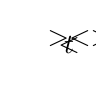
\begin{tikzpicture}
        \Tree
            [.$>$
                [.\node(VP){$<$};
                    \mlex{gehauen}{}
                    \node(object_t){$t$};
                ]
                [.$<$
                    \mlex{hat}{C}
                    [.$>$
                        [.\node(subject){$<$};
                            \mlex{der}{}
                            \mlex{Hans}{}
                        ]
                        [.$<$
                            \mlex{$\emptystring$}{}
                            [.$>$
                                [.\node(object){$<$};
                                    \mlex{die}{}
                                    \mlex{Maria}{}
                                ]
                                [.$>$
                                    \node(subject_t){$t$};
                                    [.$<$
                                        \mlex{$\emptystring$}{}
                                        \node(VP_t){$t$};
                                    ]
                                ]
                            ]
                        ]
                    ]
                ]
            ]
    \end{tikzpicture}

    \begin{tikzpicture}[
        level 1+/.style = { sibling distance = -9em },
        level 6/.style = { sibling distance = 2em },
        level 7/.style = { sibling distance = 0em },
        level 8/.style = { sibling distance = -3em },
        level 9/.style = { sibling distance = 0em }
        ]
        \Tree
            [.Move
                [.Merge
                    \mlex{hat}{\fsel{T}\ +top\ C}
                    [.Move
                        [.Merge
                            \mlex{$\emptystring$}{\fsel{\mathit{v}}\ +nom\ T}
                            [.Move
                                [.Merge
                                    [.\node(subject){Merge};
                                        \mlex{der}{\fsel{N}\ D\ -nom}
                                        \mlex{Hans}{N}
                                    ]
                                    [.Merge
                                        \mlex{$\emptystring$}{\fsel{V}\ \fsel{D}\ +acc\ \mathit{v}}
                                        [.\node(VP){Merge};
                                            \mlex{gehauen}{\fsel{D}\ V\ -top}
                                            [.\node(object){Merge};
                                                \mlex{die}{\fsel{N}\ D\ -acc}
                                                \mlex{Maria}{N}
                                            ]
                                        ]
                                    ]
                                ]
                            ]
                        ]
                    ]
                ]
            ]
    \end{tikzpicture}
\end{center}
%
At a quick glance it is actually hard to tell whether this derivation is well-formed.
That's because the derivation tree does not directly keep track of which features are still unchecked at each point of the derivation.
However, we can add this information by annotating every interior node with a tuple, each component of which is the list of unchecked features of some lexical item.
%
\begin{center}
    \begin{tikzpicture}[
        level 1+/.style = { sibling distance = -9em },
        level 6/.style = { sibling distance = 2em },
        level 7/.style = { sibling distance = 0em },
        level 8/.style = { sibling distance = -3em },
        level 9/.style = { sibling distance = 0em }
        ]
        \Tree
            [.\ftuple{C}
                [.\ftuple{+top\ C, -top}
                    \mlex{hat}{\fsel{T}\ +top\ C}
                    [.\ftuple{T, -top}
                        [.\ftuple{+nom\ T, -top, -nom}
                            \mlex{$\emptystring$}{\fsel{\mathit{v}}\ +nom\ T}
                            [.\ftuple{\mathit{v}, -top, -nom}
                                [.\ftuple{+acc\ \mathit{v}, -top, -acc, -nom}
                                    [.\ftuple{D\ -nom}
                                        \mlex{der}{\fsel{N}\ D\ -nom}
                                        \mlex{Hans}{N}
                                    ]
                                    [.\ftuple{\fsel{D}\ +acc\ \mathit{v}, -top, -acc}
                                        \mlex{$\emptystring$}{\fsel{V}\ \fsel{D}\ +acc\ \mathit{v}}
                                        [.\ftuple{V\ -top, -acc}
                                            \mlex{gehauen}{\fsel{D}\ V\ -top}
                                            [.\ftuple{D\ -acc}
                                                \mlex{die}{\fsel{N}\ D\ -acc}
                                                \mlex{Maria}{N}
                                            ]
                                        ]
                                    ]
                                ]
                            ]
                        ]
                    ]
                ]
            ]
    \end{tikzpicture}
\end{center}

Notice how the feature-annotated derivation tree can easily be described by a small number of rewrite rules:
%
\begin{center}
    \begin{tabular}{rcl}
        \ftuple{C}                                      & \rewrite & \ftuple{+top\ C, -top}\\
        \ftuple{+top\ C, -top}                          & \rewrite & \ftuple{\fsel{T}\ +top\ C} \ftuple{T, -top}\\
        \ftuple{T, -top}                                & \rewrite & \ftuple{+nom\ T, -top, -nom}\\
        \ftuple{+nom\ T, -top, -nom}                    & \rewrite & \ftuple{\fsel{\mathit{v}}\ +nom\ T} \ftuple{\mathit{v}, -top, -nom}\\
        \ftuple{\mathit{v}, -top, -nom}                 & \rewrite & \ftuple{+acc\ \mathit{v}, -top, -acc, -nom}\\
        \ftuple{+acc\ \mathit{v}, -top, -acc, -nom}     & \rewrite & \ftuple{D\ -nom} \ftuple{\fsel{D}\ +acc\ \mathit{v}, -top, -acc}\\
        \ftuple{D\ -nom}                                & \rewrite & \ftuple{\fsel{N}\ D\ -nom} \ftuple{N}\\
        \ftuple{\fsel{D}\ +acc\ \mathit{v}, -top, -acc} & \rewrite & \ftuple{\fsel{V}\ \fsel{D}\ +acc\ \mathit{v}} \ftuple{V\ -top, -acc}\\
        \ftuple{V\ -top, -acc}                          & \rewrite & \ftuple{\fsel{D}\ V\ -top} \ftuple{D\ -acc}\\
        \ftuple{D\ -acc}                                & \rewrite & \ftuple{\fsel{N}\ D\ -acc} \ftuple{N}\\[2em]
        %
        \ftuple{\fsel{T}\ +top\ C}                      & \rewrite & hat\\
        \ftuple{\fsel{\mathit{v}}\ +nom\ T}             & \rewrite & $\emptystring$\\
        \ftuple{\fsel{V}\ \fsel{D}\ +acc\ \mathit{v}}   & \rewrite & $\emptystring$\\
        \ftuple{\fsel{D}\ V\ -top}                      & \rewrite & gehauen\\
        \ftuple{\fsel{N}\ D\ -nom}                      & \rewrite & der\\
        \ftuple{\fsel{N}\ D\ -acc}                      & \rewrite & die\\
        \ftuple{N}                                      & \rewrite & Hans | Maria
    \end{tabular}
\end{center}
%
While these rewrite rules are incredibly difficult to make sense of for humans, they generate the desired derivation tree (with the minor difference that for the sake of readability every lexical item has been split into two nodes, with the phonetic exponent as the daughter of the feature component).
In fact, there is a fully automatic procedure for converting an MG $G$ with lexicon $\Lex$ into a CFG $C$ such that $C$ generates all well-formed derivation trees of $G$, and only those (this result hinges on the SMC; see \citealt{Kobele.etal07} and section 2.1.3 of \citealt{Graf13Thesis}).

Clearly every phrase structure tree is fully described by its derivation tree (or trees, if there are multiple ways of building and one and the same phrase structure tree), since the latter is a set of instructions for building the former.
This means that the structure of a sentence is completely specified by assigning it a derivation tree.
So even though an MG parser has to work for string languages that are not context-free, it still only has to assign each sentence a context-free structure -- the derivation trees.
As we will see next, this idea works fairly well, but there is one major complication: the string yield of a derivation tree does not correspond to the sentence being parsed because movement can change the order of words.

\section{Top-Down Parser with Feature Annotated Derivations}
\label{sec:MG-TopDown_Parser}

\subsection{MGs without Movement --- A Naive Top-Down Parser}
\label{sub:MG-TopDown_Naive}
For an MG without movement --- i.e.\ an MG where no lexical item has any licensee features --- designing a parser is straight-forward.
In this case, the order of the leaves in the derivation tree can be taken to mirror the order of the words in the input sentence.
So if MG $G$ is movement-free, we can translate it into a CFG that generates $G$'s derivation trees and use any one of our familiar parsers for this CFG\@.

But let's see if we can design a parser that reflects the MG feature calculus more directly.
If there are only Merge nodes in the derivation, every interior node has exactly two daughters.
In addition, all the features of the node must have been contributed by exactly one of its daughters, namely the one with the selector feature (take a minute to convince yourself that this is indeed the case!).
Since the selector may be linearized either to the left or to the right, we need two distinct inference rules.
%
\begin{prooftree}
    \AxiomC{\tuple{\alpha}}
    \LeftLabel{\textbf{Merge1}\qquad}
    \RightLabel{$F$ a feature name of $G$}
    \UnaryInfC{\tuple{\fsel{F}\ \alpha} \qquad \tuple{\mathrm{F}}}
\end{prooftree}
%
\begin{prooftree}
    \AxiomC{\tuple{\alpha}}
    \LeftLabel{\textbf{Merge2}\qquad}
    \RightLabel{$F$ a feature name of $G$}
    \UnaryInfC{\tuple{\mathrm{F}} \qquad \tuple{\fsel{F}\ \alpha}}
\end{prooftree}

There is one minor problem with those rules, though, and that's that the selector should always be to the left of its first argument, and always to the right of its other arguments.
Our rules do not capture this fact.
For example, if $\alpha$ is C then the parser could linearize the complementizer to the left or to the right of TP\@.
But an MG would only entertain the first option.
The simplest fix is to annotate each selector feature with information about how the argument is linearized, and that's the solution we will use for now.

\begin{prooftree}
    \AxiomC{\tuple{\alpha}}
    \LeftLabel{\textbf{Merge Right}\qquad}
    \RightLabel{F a feature name of $G$}
    \UnaryInfC{\tuple{\fsel{F}_r\ \alpha} \qquad \tuple{\mathrm{F}}}
\end{prooftree}
%
\begin{prooftree}
    \AxiomC{\tuple{\alpha}}
    \LeftLabel{\textbf{Merge Left}\qquad}
    \RightLabel{F a feature name of $G$}
    \UnaryInfC{\tuple{\mathrm{F}} \qquad \tuple{\fsel{F}_l\ \alpha}}
\end{prooftree}

The only thing remaining, then, is a rule for the removal of lexical items, similar to the scan rule.
%
\begin{prooftree}
    \AxiomC{\tuple{\alpha}}
    \LeftLabel{\textbf{LI}\qquad}
    \RightLabel{$\mlex{w}{\alpha} \in \Lex_G$}
    \UnaryInfC{}
\end{prooftree}

\subsection{Recursive Descent Parser for Movement-Free MGs}
\label{sub:MG-TopDown_Movement-Free}
The previous discussion is sufficient to outline the feature-based logic of an MG parser, but it does not serve as a parsing schema.
Just like in recursive descent parsing, our parsing items need to keep track of all the non-terminal symbols and put the in the right linear order.
This, however, is very simply to do.
%
For a recursive-descent MG parser, the only axiom is $[0,\psep \ftuple{C}]$, and the only goal is $[n,\psep]$.
%
\begin{prooftree}
    \AxiomC{$[i,\psep \tuple{\alpha} \beta, j]$}
    \LeftLabel{\textbf{Merge Left}\qquad}
    \RightLabel{F a feature name of $G$}
    \UnaryInfC{$[i,\psep \tuple{\mathrm{F}} \tuple{\fsel{F}_l\ \alpha} \beta, j]$}
\end{prooftree}
%
\begin{prooftree}
    \AxiomC{$[i,\psep \tuple{\alpha} \beta, j]$}
    \LeftLabel{\textbf{Merge Right}\qquad}
    \RightLabel{F a feature name of $G$}
    \UnaryInfC{$[i,\psep \tuple{\fsel{F}_r\ \alpha} \tuple{\mathrm{F}} \beta, j]$}
\end{prooftree}
%
\begin{prooftree}
    \AxiomC{$[i,\psep \tuple{\alpha} \beta, j]$}
    \LeftLabel{\textbf{LI (pronounced)}\qquad}
    \RightLabel{$\mlex{$w_i$}{\alpha} \in \Lex_G$, $w_i \neq \emptystring$}
    \UnaryInfC{$[i+1,\psep \beta, j]$}
\end{prooftree}
%
\begin{prooftree}
    \AxiomC{$[i,\psep \tuple{\alpha} \beta, j]$}
    \LeftLabel{\textbf{LI (empty)}\qquad}
    \RightLabel{$\mlex{$w_i$}{\alpha} \in \Lex_G$, $w_i = \emptystring$}
    \UnaryInfC{$[i,\psep \beta, j]$}
\end{prooftree}

\begin{examplebox}[MG Top-Down Parse of \emph{The man likes Mary}]
    Suppose the sentence \emph{The man likes Mary} has the structure below.
    %
    \begin{center}
        \begin{tikzpicture}
            \Tree
                [.CP
                    C
                    [.VP
                        [.DP
                            the
                            man
                        ]
                        [.V$'$
                            likes
                            [.DP
                                Mary
                            ]
                        ]
                    ]
                ]
        \end{tikzpicture}
    \end{center}
    %
    The feature-annotated Minimalist derivation tree for this sentence looks as follows.
    %
    \begin{center}
        \begin{tikzpicture}
            \Tree
                [.\ftuple{C}
                    \mlex{\emptystring}{\fsel{V}_r\ C}
                    [.\ftuple{V}
                        [.\ftuple{D}
                            \mlex{the}{\fsel{N}_r\ D}
                            \mlex{man}{N}
                        ]
                        [.\ftuple{\fsel{D}_l\ V}
                            \mlex{likes}{\fsel{D}_r\ \fsel{D}_l\ V}
                            \mlex{Mary}{D}
                        ]
                    ]
                ]
        \end{tikzpicture}
    \end{center}
    %
    The parse table directly reflects this structure.
    %
    \begin{center}
        \begin{tabular}{r|l}
            \textbf{parse item} & \textbf{inference rule}\\
                $\lbrack$0, \psep \ftuple{C}] & axiom\\
                $\lbrack$0, \psep \ftuple{\fsel{V}_r\ C} \ftuple{V}] & Merge Right\\
                $\lbrack$0, \psep \ftuple{V}] & LI (empty)\\
                $\lbrack$0, \psep \ftuple{D} \ftuple{\fsel{D}_l\ V}] & Merge Left\\
                $\lbrack$0, \psep \ftuple{\fsel{N}\ D} \ftuple{N} \ftuple{\fsel{D}_l\ V}] & Merge Right\\
                $\lbrack$1, \psep \ftuple{N} \ftuple{\fsel{D}_l\ V}] & LI (pronounced)\\
                $\lbrack$2, \psep \ftuple{\fsel{D}_l\ V}] & LI (pronounced)\\
                $\lbrack$2, \psep \ftuple{\fsel{D}_r \fsel{D}_l\ V} \ftuple{D}] & Merge Right\\
                $\lbrack$3, \psep \ftuple{D}] & LI (pronounced)\\
                $\lbrack$4, \psep ] & LI (pronounced)\\
        \end{tabular}
    \end{center}
    %
    We can annotate the final derivation tree as usual to indicate how it is built by the parser.
    %
    \begin{center}
        \begin{tikzpicture}
            \Tree
                [.\Lab{Merge}{1}{2}
                    \Lab{\mlex{\emptystring}{\fsel{V}_r\ C}}{2}{3}
                    [.\BLab{Merge}{2}{4}
                        [.\Lab{Merge}{4}{5}
                            \Lab{\mlex{the}{\fsel{N}_r\ D}}{5}{6}
                            \BLab{\mlex{man}{N}}{5}{7}
                        ]
                        [.\BLab{\ftuple{\fsel{D}_l\ V}}{4}{8}
                            \Lab{\mlex{likes}{\fsel{D}_r\ \fsel{D}_l\ V}}{8}{9}
                            \BLab{\mlex{Mary}{D}}{8}{10}
                        ]
                    ]
                ]
        \end{tikzpicture}
    \end{center}
\end{examplebox}

\subsection{Adding Movement}
\label{sub:MG-TopDown_Movement}
In principle, movement inference rules aren't all that different from Merge inference rules: we have a given expression of features, and infer which expressions this could have been produced from.
But there are three important differences:
%
\begin{itemize}
    \item Move is a unary rule, so we go from $\ftuple{\alpha}$ to $\ftuple{\beta}$, where $\beta$ differs minimally from $\alpha$,
    \item a tuple can now contain multiple feature strings, all but one of which are sequences of licensee features,
    \item we need a way to incorporate how Move changes the linear order of lexical items.
\end{itemize}
%
Let's deal with points 1 and 2 first.
In general, our feature tuples will now have the form $\ftuple{\alpha, \beta_1, \ldots, \beta_n}$, where each $\beta_i$ is a string of licensee features.
This means that we have to slightly change our Merge rules.
%
\begin{prooftree}
    \AxiomC{\tuple{\alpha, \beta_1, \ldots, \beta_n}}
    \LeftLabel{\textbf{Merge Right}\qquad}
    \RightLabel{F a feature name of $G$}
    \UnaryInfC{\tuple{\fsel{F}_r\ \alpha, \gamma_1, \ldots, \gamma_k} \qquad \tuple{\mathrm{F} \delta, \gamma_{k+1}, \ldots, \gamma_n}}
\end{prooftree}
%
\begin{prooftree}
    \AxiomC{\tuple{\alpha, \beta_1, \ldots, \beta_n}}
    \LeftLabel{\textbf{Merge Left}\qquad}
    \RightLabel{F a feature name of $G$}
    \UnaryInfC{\tuple{\mathrm{F} \delta, \gamma_1, \ldots, \gamma_k} \qquad \tuple{\fsel{F}_l\ \alpha, \gamma_{k+1}, \ldots, \gamma_n}}
\end{prooftree}
%
Notice that we now distribute the strings of licensee features over the two daughters of a Merge node in a non-deterministic fashion.
That is to say, we require in both rules that
%
\begin{itemize}
    \item for all $1 \leq i, j \leq n$, the first features of $\beta_i$ and $\beta_j$ are distinct,
    \item if $\delta = \emptystring$, then each $\beta_i$ is identical to exactly one $\gamma_j$, and \emph{vice versa},
    \item otherwise, there is some $\beta_i$ such that $\beta_i = \delta$ and the previous condition holds for all $\beta_j$ with $j \neq i$.
\end{itemize}

The logic of the movement rule is even simpler.
%
\begin{prooftree}
    \AxiomC{\tuple{\alpha, \beta_1, \ldots, \beta_i, \ldots, \beta_n}}
    \LeftLabel{\textbf{Move}\qquad}
    \RightLabel{$\mathrm{-f}$ a licensee feature of $G$}
    \UnaryInfC{\tuple{\mathrm{+f}\ \alpha, \beta_1, \ldots, \mathrm{-f}\ \beta_i, \ldots, \beta_n}}
\end{prooftree}
%
Notice that $\beta_i$ may be empty.
In that case, we are dealing with the final landing site of whichever lexical item hosts the $\mathrm{-f}$ feature.
Strictly speaking, then, the item in the antecedent line of the rule would have two adjacent commas with nothing inbetween the two since $\beta_i$ is empty.
Our rules never create an item of this form, so the Move rule couldn't apply in this case.
Hence we should actually distinguish two cases of movement.

\begin{prooftree}
    \AxiomC{\tuple{\alpha, \beta_1, \ldots, \beta_i, \ldots, \beta_n}}
    \LeftLabel{\textbf{Move (intermediate)}\qquad}
    \RightLabel{$\mathrm{-f}$ a licensee feature of $G$}
    \UnaryInfC{\tuple{\mathrm{+f}\ \alpha, \beta_1, \ldots, \mathrm{-f}\ \beta_i, \ldots, \beta_n}}
\end{prooftree}
%
\begin{prooftree}
    \AxiomC{\tuple{\alpha, \beta_1, \ldots, \beta_{i-1}, \beta_{i+1} \ldots, \beta_n}}
    \LeftLabel{\textbf{Move (final)}\qquad}
    \RightLabel{$\mathrm{-f}$ a licensee feature of $G$}
    \UnaryInfC{\tuple{\mathrm{+f}\ \alpha, \beta_1, \ldots, \beta_{i-1}, \mathrm{-f}, \beta_{i+1} \ldots, \beta_n}}
\end{prooftree}

These movement rules do not take care of the true challenge posed by movement however, and that's keeping track of the order of words in the sentence, which no longer corresponds to the order of words in the derivation tree.
Assume that we conjecture a Move node for topicalization.
Then we have to keep track of the fact that we expect to see an LI later on, which is handled by the presence of $\mathrm{-f}$ or $\mathrm{-f}\ \beta_i$ in the tuples.
But we also need to know that once we have found this item, the phrase it is a head of should match a sequence of words at the position where we initially conjectured topicalization movement.

\subsection{Keeping Track of Conjectured Movers}
\label{sub:MG-TopDown_MoveIndices}
In order to keep track of which positions in the string are associated with movers, we use place holders of the form $[f]$, where $f$ is a feature name.
These place holders are introduced by Move rules and allow us to reorder the tuples in a parse item where possible.
Given a substring $\phi$ of a parse item, $\phi_{/[f_1 \cdots f_n]}$ is the result of removing the placeholders $[f_1]$, \ldots, $[f_n]$ from $\phi$.

Once again the axiom is $[0,\psep \ftuple{C}]$ and the goal is $[n,\psep]$.
We need 4 Merge rule, 2 Move rules, and a few ancillary rules.
The Merge rules are parameterized according to linearization and whether the merged item is a mover.
%
\begin{prooftree}
    \AxiomC{$[i,
        \phi \psep
        \tuple{\alpha, \beta_1, \ldots, \beta_n}
        \psi
        ]$}
    \LeftLabel{\textbf{Merge Right}\qquad}
    \UnaryInfC{$[i,
        \phi
        \psep
        \tuple{\fsel{F}_r\ \alpha, \gamma_1, \ldots, \gamma_k}
        \tuple{\mathrm{F} \delta, \gamma_{k+1}, \ldots, \gamma_n}
        \psi
        ]$}
\end{prooftree}
%
\begin{prooftree}
    \AxiomC{$[i,
        \phi
        \psep
        \tuple{\alpha, \beta_1, \ldots, \beta_n}
        \psi
        ]$}
    \LeftLabel{\textbf{Merge Left}\qquad}
    \UnaryInfC{$[i,
        \phi
        \psep
        \tuple{\mathrm{F} \delta, \gamma_{k+1}, \ldots, \gamma_n}
        \tuple{\fsel{F}_l\ \alpha, \gamma_1, \ldots, \gamma_k}
        \psi
        ]$}
\end{prooftree}
%
\noindent
\textbf{Merge Mover Right}
\begin{prooftree}
    \AxiomC{$[i,
        \phi \psep
        \tuple{\alpha, \beta_1, \ldots, f_1 \cdots f_m, \beta_n}
        \psi
        ]$}
    \UnaryInfC{$[i,
        \phi_{/[f_1 \cdots f_{m-1}]}
        \psep
        \tuple{\fsel{F}_r\ \alpha, \gamma_1, \ldots, \gamma_{k-1}}
        [_{f_m} \tuple{\mathrm{F}\ f_1 \cdots f_m , \gamma_{k+1}, \ldots, \gamma_n}]
        \psi_{/[f_1 \cdots f_{m-1}]}
        ]$}
\end{prooftree}
%
\noindent
\textbf{Merge Mover Left}
\begin{prooftree}
    \AxiomC{$[i,
        \phi
        \psep
        \tuple{\alpha, \beta_1, \ldots, f_1 \cdots f_m , \ldots \beta_n}
        \psi
        ]$}
    \UnaryInfC{$[i,
        \phi_{/[f_1 \cdots f_{m-1}]}
        \psep
        [_{f_m} \tuple{\mathrm{F} f_1 \cdots f_n, \gamma_{k+1}, \ldots, \gamma_n}]
        \tuple{\fsel{F}_l\ \alpha, \gamma_1, \ldots, \gamma_{k-1}}
        \psi_{/[f_1 \cdots f_{m-1}]}
        ]$}
\end{prooftree}
%
The $f$-subscripted brackets around a tuple mark it as an $f$-mover, which is necessary to identify it with the right placeholder in $\phi$ or $\psi$.
Notice also that we eliminate all placeholders for intermediate movement as soon as the mover is merged.
Since the mover will never occur at an intermediate landing site --- after all, it has to move to its final target position --- those placeholders are string vacuous.
However, we have to introduce them first to make sure that the feature checking requirements are satisfied: every non-final licensee feature needs a corresponding move node, which corresponds to a placeholder in the parse item.

\begin{prooftree}
    \AxiomC{$[i,
        \phi
        \psep
        \tuple{\alpha, \beta_1, \ldots, \beta_i, \ldots, \beta_n}
        \psi
        ]$}
    \LeftLabel{\textbf{Move (intermediate)}\qquad}
    \UnaryInfC{$[i,
        \phi
        [\mathrm{f}]
        \psep
        \tuple{\mathrm{+f}\ \alpha, \beta_1, \ldots, \mathrm{-f}\ \beta_i, \ldots, \beta_n}
        \psi
        ]$}
\end{prooftree}
%
\begin{prooftree}
    \AxiomC{$[i,
        \phi
        \psep
        \tuple{\alpha, \beta_1, \ldots, \beta_{i-1}, \beta_{i+1} \ldots, \beta_n}
        \psi
        ]$}
    \LeftLabel{\textbf{Move (final)}\qquad}
    \UnaryInfC{$[i,
        \phi
        [\mathrm{f}]
        \psep
        \tuple{\mathrm{+f}\ \alpha, \beta_1, \ldots, \beta_{i-1}, \mathrm{-f}, \beta_{i+1} \ldots, \beta_n}
        \psi
        ]$}
\end{prooftree}
%
The Move rules are almost exactly the same, except that Move (intermediate) extends an existing $\beta_i$, whereas Move (final) adds a completely new one.

The actual reordering of tuples in a parse item is handled by the rule displace, which takes a mover and puts it in the position of the placeholder.
%
\begin{prooftree}
    \AxiomC{$[i,
        \phi [f] \phi'
        \psep
        [_f \alpha ]
        \psi
        ]$}
    \LeftLabel{\textbf{Displace Left}\qquad}
    \UnaryInfC{$[i,
        \phi \psep \alpha \phi'
        \psi
        ]$}
\end{prooftree}
%
\begin{prooftree}
    \AxiomC{$[i,
        \phi
        \psep
        [_f \alpha ]
        \psi
        [f]
        \psi'
        ]$}
    \LeftLabel{\textbf{Displace Right}\qquad}
    \UnaryInfC{$[i,
        \phi \psep \psi \alpha 
        \psi'
        ]$}
\end{prooftree}

The LI rule replaces a feature tuple by an LI with that feature specification, and the scan rule eliminates LIs from the parse items.
Scanning an LI is allowed only if it is at the very left edge of the parse item.
%
\begin{prooftree}
    \AxiomC{$[i,\phi \psep \tuple{\alpha} \psi]$}
    \LeftLabel{\textbf{LI}\qquad}
    \RightLabel{$\mlex{$a$}{\alpha} \in \Lex_G$}
    \UnaryInfC{$[i,\phi \psep a \psi]$}
\end{prooftree}
%
\begin{prooftree}
    \AxiomC{$[i,\psep a \beta]$}
    \LeftLabel{\textbf{Scan}\qquad}
    \RightLabel{$k = i$ if $a = \emptystring$ and $i+1$ otherwise}
    \UnaryInfC{$[k,\psep \beta]$}
\end{prooftree}

The shift rule moves $\psep$ to the right if no other rule can be applied.
%
\begin{prooftree}
    \AxiomC{$[i,
        \phi
        \psep x \psi
        ]$}
    \LeftLabel{\textbf{Shift}\qquad}
    \RightLabel{$\phi$ not the empty string, $x$ a placeholder or an LI}
    \UnaryInfC{$[i,
        \phi x
        \psep \psi
        ]$}
\end{prooftree}

\begin{examplebox}[MG Top-Down Parse of \emph{Gehauen hat die Maria der Hans}]
    Let's look at a slightly more complicated version of our very first example sentence.
    %
    \begin{exe}
        \ex
            {\gll Gehauen hat die Maria der Hans.\\
                  beaten has the Maria the Hans\\
            }
    \end{exe}
    %
    Here the object \emph{die Maria} not only moves out of the VP, but it also scrambles across the subject \emph{der Hans} afterwards.
    A simplified derivation tree is given below.
    %
    \begin{center}
        \begin{tikzpicture}
            \begin{scope}
                \tikzset{    
                    level 1+/.style = { sibling distance = -9em },
                    level 5+/.style = { sibling distance = 2em },
                }
                \Tree
                    [.\ftuple{C}
                        [.\ftuple{+top\ C, -top}
                            \mlex{hat}{\fsel{T}\ +top\ C}
                            [.\ftuple{T, -top}
                                [.\ftuple{+f\ T, -top, -f}
                                    [.\ftuple{+nom\ +f\ T, -top, -f, -nom}
                                        \mlex{$\emptystring$}{\fsel{\mathit{v}}\ +nom\ +f\ T}
                                        [.\ftuple{\mathit{v}, -top, -f, -nom}
                                            [.\ftuple{+acc\ \mathit{v}, -top, -acc\ -f, -nom}
                                                [.\ftuple{D\ -nom}
                                                    \mlex{der}{\fsel{N}\ D\ -nom}
                                                    \mlex{Hans}{N}
                                                ]
                                                \node(bottom){\phantom{bottom}};
                                            ]
                                        ]
                                    ]
                                ]
                            ]
                        ]
                    ]
            \end{scope}

            \begin{scope}[yshift=-27em]
                \Tree
                    [.\node(top){\ftuple{\fsel{D}\ +acc\ \mathit{v}, -top, -acc\ -f}};
                        \mlex{$\emptystring$}{\fsel{V}\ \fsel{D}\ +acc\ \mathit{v}}
                        [.\ftuple{V\ -top, -acc\ -f}
                            \mlex{gehauen}{\fsel{D}\ V\ -top}
                            [.\ftuple{D\ -acc\ -f}
                                \mlex{die}{\fsel{N}\ D\ -acc\ -f}
                                \mlex{Maria}{N}
                            ]
                        ]
                    ]
            \end{scope}

            \draw (top.north) .. controls +(45:2em) and +(270:8em) .. (bottom.north);
        \end{tikzpicture}
    \end{center}
    
    The parser infers the derivation with the following steps.
    %
    \begin{center}
        \small
        \begin{longtable}{r|l}
            \textbf{parse item} & \textbf{inference rule}\\
                $\lbrack$0, \psep \ftuple{C}] & axiom\\
                $\lbrack$0, [top] \psep \ftuple{+top\ C, -top}] & Move (final)\\
                $\lbrack$0, [top] \psep \ftuple{\fsel{T}\ +top\ C} \ftuple{T, -top}]  & Merge Right\\
                $\lbrack$0, [top] hat \psep \ftuple{T, -top}]  & LI \& Shift\\[.5em]
                %
                $\lbrack$0, [top] hat [f] &\\
                \psep \ftuple{+f\ T, -top, -f}]  & Move (final)\\[.5em]
                %
                $\lbrack$0, [top] hat [f] [nom] &\\
                \psep \ftuple{+nom\ +f\ T, -top, -f, -nom}] & Move (final)\\[.5em]
                %
                $\lbrack$0, [top] hat [f] [nom] &\\
                \psep \ftuple{\fsel{\mathit{v}}\ +nom\ +f\ T} \ftuple{\mathit{v}, -top, -f, -nom}] & Merge Right\\[.5em]
                %
                $\lbrack$0, [top] hat [f] [nom] \emptystring &\\
                \psep \ftuple{\mathit{v}, -top, -f, -nom}] & LI \& Shift\\[.5em]
                %
                $\lbrack$0, [top] hat [f] [nom] \emptystring\ [acc] \\
                \psep \ftuple{+acc\ \mathit{v}, -top, -acc\ -f, -nom}] & Move (intermediate)\\[.5em]
                %
                $\lbrack$0, [top] hat [f] [nom] \emptystring\ [acc] \\
                \psep [\tsb{nom} \ftuple{D\ -nom}] \ftuple{\fsel{D}\ +acc\ \mathit{v}, -top, -acc\ -f}] & Merge Mover Left\\[.5em]
                %
                $\lbrack$0, [top] hat [f] \psep \ftuple{D\ -nom} \emptystring\ [acc]\\
                \ftuple{\fsel{D}\ +acc\ \mathit{v}, -top, -acc\ -f}] & Displace Left\\[.5em]
                %
                $\lbrack$0, [top] hat [f] \psep \ftuple{\fsel{N}\ D\ -nom} \ftuple{N} \emptystring\ [acc]\\ 
                 \ftuple{\fsel{D}\ +acc\ \mathit{v}, -top, -acc\ -f}] & Merge Right\\[.5em]
                %
                $\lbrack$0, [top] hat [f] der \psep \ftuple{N} [f] [nom] \emptystring\ [acc]\\
                \ftuple{\fsel{D}\ +acc\ \mathit{v}, -top, -acc\ -f}] & LI \& Shift\\[.5em]
                %
                $\lbrack$0, [top] hat [f] der Hans \psep \emptystring\ [acc]\\
                \ftuple{\fsel{D}\ +acc\ \mathit{v}, -top, -acc\ -f}] & LI \& Shift\\[.5em]
                %
                $\lbrack$0, [top] hat [f] der Hans \emptystring\ [acc]\\
                \psep \ftuple{\fsel{D}\ +acc\ \mathit{v}, -top, -acc\ -f}] & Shift*2\\[.5em]
                %
                $\lbrack$0, [top] hat [f] der Hans \emptystring\ [acc]\\
                \psep \ftuple{\fsel{V}\ \fsel{D}\ +acc\ \mathit{v}} [\tsb{top} \ftuple{V\ -top, -acc\ -f}]] & Merge Mover Right\\[.5em]
                %
                $\lbrack$0, [top] hat [f] der Hans \emptystring\ [acc] \emptystring\\
                \psep [\tsb{top} \ftuple{V\ -top, -acc\ -f}]] & LI \& Shift\\[.5em]
                %
                $\lbrack$0, \psep \ftuple{V\ -top, -acc\ -f} hat [f] der Hans \emptystring\ [acc] \emptystring] & Displace Left\\[.5em]
                %
                $\lbrack$0, \psep \ftuple{\fsel{D}\ V\ -top} [\tsb{f} \ftuple{D\ -acc\ -f}]\\
                hat [f] der Hans \emptystring\ \emptystring] & Merge Mover Right\\[.5em]
                %
                $\lbrack$0, \psep gehauen [\tsb{f} \ftuple{D\ -acc\ -f}]\\
                hat [f] der Hans \emptystring\ \emptystring] & LI\\[.5em]
                %
                $\lbrack$1, \psep [\tsb{f} \ftuple{D\ -acc\ -f}]\\
                hat [f] der Hans \emptystring\ \emptystring] & Scan\\[.5em]
                %
                $\lbrack$1, \psep 
                hat \ftuple{D\ -acc\ -f} der Hans \emptystring\ \emptystring] & Displace Right\\[.5em]
                %
                $\lbrack$2, \psep 
                \ftuple{D\ -acc\ -f} der Hans \emptystring\ \emptystring] & Scan\\[.5em]
                %
                $\lbrack$2, \psep 
                \ftuple{\fsel{N}\ D\ -acc\ -f} \ftuple{N} der Hans \emptystring\ \emptystring] & Merge Right\\[.5em]
                %
                $\lbrack$2, \psep 
                die \ftuple{N} der Hans \emptystring\ \emptystring] & LI\\[.5em]
                %
                $\lbrack$3, \psep 
                \ftuple{N} der Hans \emptystring\ \emptystring] & Scan\\[.5em]
                %
                $\lbrack$3, \psep 
                Maria der Hans \emptystring\ \emptystring] & LI\\[.5em]
                %
                $\lbrack$4, \psep 
                der Hans \emptystring\ \emptystring] & Scan\\
                %
                $\lbrack$5, \psep 
                Hans \emptystring\ \emptystring] & Scan\\
                %
                $\lbrack$6, \psep 
                \emptystring\ \emptystring] & Scan\\
                %
                $\lbrack$6, \psep 
                \emptystring] & Scan\\
                %
                $\lbrack$6, \psep 
                ] & Scan\\
        \end{longtable}
    \end{center}

    We can represent this parse more succinctly by annotating the derivation tree with indices in the usual fashion.
    %
    \begin{center}
        \begin{tikzpicture}
            \begin{scope}
                \tikzset{    
                    level 1+/.style = { sibling distance = -9em },
                    level 6+/.style = { sibling distance = 0em },
                }
                \Tree
                    [.\Lab{Move}{1}{2}
                        [.\Lab{Merge}{2}{3}
                            \BLab{\mlex{hat}{\fsel{T}\ +top\ C}}{3}{13}
                            [.\Lab{Move}{3}{4}
                                [.\Lab{Move}{4}{5}
                                    [.\Lab{Merge}{5}{6}
                                        \BLab{\mlex{\emptystring}{\fsel{\mathit{v}}\ +nom\ +f\ T}}{6}{19}
                                        [.\Lab{Move}{6}{7}
                                            [.\Lab{Merge}{7}{8}
                                                [.\Lab{Merge}{8}{9}
                                                    \BLab{\mlex{der}{\fsel{N}\ D\ -nom}}{9}{17}
                                                    \BLab{\mlex{Hans}{N}}{9}{18}
                                                ]
                                                \node(bottom){\phantom{bottom}};
                                            ]
                                        ]
                                    ]
                                ]
                            ]
                        ]
                    ]
            \end{scope}

            \begin{scope}[yshift=-27em]
                \tikzset{
                    level 1+/.style = { sibling distance = -5em },
                    level 3/.style = { sibling distance = 0em}
                }
                \Tree
                    [.\node(top){\BLab{Merge}{8}{10}};
                        \BLab{\mlex{$\emptystring$}{\fsel{V}\ \fsel{D}\ +acc\ \mathit{v}}}{10}{20}
                        [.\Lab{Merge}{10}{11}
                            \Lab{\mlex{gehauen}{\fsel{D}\ V\ -top}}{11}{12}
                            [.\BLab{Merge}{11}{14}
                                \Lab{\mlex{die}{\fsel{N}\ D\ -acc\ -f}}{14}{15}
                                \BLab{\mlex{Maria}{N}}{14}{16}
                            ]
                        ]
                    ]
            \end{scope}

            \draw (top.north) .. controls +(45:2em) and +(270:12em) .. (bottom.north);
        \end{tikzpicture}
    \end{center}
\end{examplebox}

\subsection{Two Issues}
\label{sub:MG-TopDown_Issues}
The parser as defined in the previous section has two issues.
First, the Merge and Move rules are only limited by the requirement that the features $\mathrm{F}$ or $\mathrm{f}$ must be valid features of the grammar.
This, however, can still lead to conjecturing tuples that could never be derived from the LIs of the grammar.
These parses will eventually fail, of course, but for efficiency reasons it would be nice if the parser would not conjecture items that can never occur in a well-formed derivation.

If we translate the MG into a CFG, the set of valid tuples corresponds to the set non-terminals of the CFG.
So with a little bit of processing, the rules can be limited to only use non-terminals of this CFG\@.
It would be more appealing, however, if we could phrase our inference rules in a way so that they operate directly on the lexicon of our MG\@.
This is exactly what is done in \citet{Stabler12}.

\posscitet{Stabler12} parser also fixes another problem with the current model.
Right now, our parser does not sufficiently prioritize the search for movers.
Since scanning of an LI $l$ is delayed until all movers to the left of $l$ have been found, memory usage would be minimized by searching for those movers.
So once the parser stipulates the presence of a top-mover in the example above, it should first follow the branches that it believes will lead it to this mover.
Once this mover has been found, it can scan \emph{hat} and then continue it's search for an $\mathrm{f}$-mover, and then for a nom-mover.
Instead, our parser starts building the nom-mover before it has even found the top-mover; this increases the memory burden because there is no way the nom-mover could be fully scanned at this point.

\begin{examplebox}[A More Efficient Traversal of the Derivation Tree]
    Using the search strategy outlined in \citet{Stabler12}, the derivation tree from the previous example would be explored in the following order.

    \begin{center}
        \begin{tikzpicture}
            \begin{scope}
                \tikzset{    
                    level 1+/.style = { sibling distance = -9em },
                    level 6+/.style = { sibling distance = 0em },
                }
                \Tree
                    [.\Lab{Move}{1}{2}
                        [.\Lab{Merge}{2}{3}
                            \BLab{\mlex{hat}{\fsel{T}\ +top\ C}}{3}{12}
                            [.\Lab{Move}{3}{4}
                                [.\Lab{Move}{4}{5}
                                    [.\Lab{Merge}{5}{6}
                                        \BLab{\mlex{\emptystring}{\fsel{\mathit{v}}\ +nom\ +f\ T}}{6}{19}
                                        [.\Lab{Move}{6}{7}
                                            [.\Lab{Merge}{7}{8}
                                                [.\BLab{Merge}{8}{16}
                                                    \Lab{\mlex{der}{\fsel{N}\ D\ -nom}}{16}{17}
                                                    \BLab{\mlex{Hans}{N}}{16}{18}
                                                ]
                                                \node(bottom){\phantom{bottom}};
                                            ]
                                        ]
                                    ]
                                ]
                            ]
                        ]
                    ]
            \end{scope}

            \begin{scope}[yshift=-27em]
                \tikzset{
                    level 1+/.style = { sibling distance = -5em },
                    level 3/.style = { sibling distance = 0em}
                }
                \Tree
                    [.\node(top){\Lab{Merge}{8}{9}};
                        \BLab{\mlex{$\emptystring$}{\fsel{V}\ \fsel{D}\ +acc\ \mathit{v}}}{9}{20}
                        [.\Lab{Merge}{9}{10}
                            \Lab{\mlex{gehauen}{\fsel{D}\ V\ -top}}{10}{11}
                            [.\BLab{Merge}{10}{13}
                                \Lab{\mlex{die}{\fsel{N}\ D\ -acc\ -f}}{13}{14}
                                \BLab{\mlex{Maria}{N}}{13}{15}
                            ]
                        ]
                    ]
            \end{scope}

            \draw (top.north) .. controls +(45:2em) and +(270:12em) .. (bottom.north);
        \end{tikzpicture}
    \end{center}
    
    The Stabler parser has a lower payload because it does not fully expand the subject right away and instead moves on to the VP first.
    If the subject contained more than two LIs, the difference in payload would be even bigger.
    Maximum tenure stays the same because it is incurred at the T-head, which is introduced before the two parser diverge in their search path and cannot be scanned until the subject has been built and scanned.
    For this reason, the differences between the two parsers do not affect the node's tenure.
    We see a marked difference in summed tenure, however, because of the tenure contributed by \emph{der} and \emph{Hans}.
    %
    \begin{center}
        \begin{tabular}{rcc}
            \textbf{Metric} & \textbf{CF Parser} & \textbf{Stabler Parser}\\
            Payload & 8 & 7\\
            MaxTen & 13 & 13\\
            SumTen & 57 & 48
        \end{tabular}
    \end{center}
\end{examplebox}
%
\begin{exercise}
    Draw a movement-free Minimalist derivation tree for \emph{The anvil hit Daffy}.
    Assume a C-T-V spine where the subject is merged as the second argument of the T-head.
    The write down the parse table and annotate the derivation tree accordingly.
    Does the parser's behavior differ noticeably from what we observed for the recursive descent parser in Chapter~\ref{cha:TopDown}?
\end{exercise}
%
\begin{exercise}
    Following up on the previous exercise, assume that we actually have a C-T-$v$-V spine where the subject starts in Spec,$v$P and then moves to Spec,TP\@.
    Once again you have to write down the parse table and annotate the derivation tree.
    What differences do you observe?
\end{exercise}

\begin{exercise}
    Draw Minimalist derivation trees for our left-embedding and right-embedding analyses of \emph{John's father's car's exhaust pipe} disappeared.
    Assume a C-T-$v$-V spine where the subject moves from Spec,$v$P to Spec,TP\@.
    Then write down the parse table for each structure. 
    Annotate the derivation trees according to how our parser would build them.
    Is the behavior of our parser similar to that of the recursive descent parser?
\end{exercise}

\bibliographystyle{../../linquiry3}
\bibliography{../../universal,../../graf}

\chapter{A Move-Eager Parser for MGs}
\label{cha:StablerParser}

The context-free parser for MGs has two disadvantages.
First, it freely infers feature tuples, with the only restriction being that the features of these tuples are features of the grammar.
Consequently, the parser may conjecture tuples that never occur in a well-formed derivation of the grammar, which is a major waste of resources.
Second, its search through the tree is not contingent on conjectured landing sites.
The parser follows a simple pattern of ``specifiers before complements'' pattern, with the minor twist that if a mover is found, the parser inserts it at the final target site and continues parsing from there.
This means that the parser has to store a lot of material in memory.
If it progressed on the most direct path to where it expects the mover to originate, without building any of the structure along the other paths, it may safe quite some resources.
Let's call the first type of parser \emph{Merge-eager}, and the second \emph{Move-eager}.
The top-down MG parser defined in \citet{Stabler12} is Move-eager and operates directly on the lexicon, which prevents it from conjecturing useless feature tuples.

\section{A Closer Look at the Stabler Parser}
See the paper for details, in particular the appendix.
The crucial insights are as follows:
%
\begin{itemize}
    \item Every Minimalist lexicon can be represented as a \emph{prefix tree}, where the prefixes correspond to the feature components of lexical items read from right to left.
    \item The prefix tree guides the parser in the structure building process.
    \item In order to deal with non-determinism, the parser keeps multiple parses in memory.
    \item Parses are ordered by their probability, and those with a probability below a fixed threshold $p$ are discarded.
        This is called \emph{beam parsing}.
    \item Since the probability of a tree decreases with every level of embedding, left branch recursion is no longer a problem for the parser.
        Instead of adding more and more levels of embedding \emph{ad infinitum}, the parser eventually reaches the probability threshold $p$ and conjectures no further levels.
\end{itemize}

\section{Psycholinguistic Adequacy}
\subsection{Generalizations about Relative Clauses}
Two major properties of relative clauses are firmly established in the literature (see \citealt{Gibson98} and references therein).
%
\begin{itemize}
    \item \textbf{SC\slash RC $<$ RC\slash SC}\\
        A sentential complement containing a relative clause is easier to process than a relative clause containing a sentential complement.
    \item \textbf{SubjRC $<$ ObjRC}\\
        A relative clause containing a subject gap is easier to parse than a relative clause containing an object gap.
\end{itemize}
%
These generalizations were obtained via self-paced reading experiments and ERP studies with minimal pairs such as \eqref{ex:StablerParser_SC/RC-RC/SC} and \eqref{ex:StablerParser_SubjRC-ObjRC}, respectively.
%
\begin{exe}
    \ex\label{ex:StablerParser_SC/RC-RC/SC}
    \begin{xlist}
        \ex The fact [\textsubscript{SC} that the employee$_i$ [\textsubscript{RC} who the manager hired $t_i$] stole office supplies] worried the executive.
        \label{ex:StablerParser_SC/RC}
        %
        \ex The executive$_i$ [\textsubscript{RC} who the fact [\textsubscript{SC} that the employee stole offices supplies] worried $t_i$] hired the manager.
        \label{ex:StablerParser_RC/SC}
    \end{xlist}
    %
    \ex\label{ex:StablerParser_SubjRC-ObjRC}
    \begin{xlist}
        \ex The reporter$_i$ [\textsubscript{RC} who $t_i$ attacked the senator] admitted the error.
        \label{ex:StablerParser_SubjRC}
        \ex The reporter$_i$ [\textsubscript{RC} who the senator attacked $t_i$] admitted the error.
        \label{ex:StablerParser_ObjRC}
    \end{xlist}
\end{exe}
%
We can use these sentences as test cases to determine whether the two types of MG parsers --- Merge-eager and Move-eager --- can account for these discrepancies, and if so, which one of them.

\subsection{Refining our Metrics}
In previous evaluations of parser predictions we used three metrics: payload for the number of nodes kept in memory, MaxTen for the maximum number of steps a node is kept in memory, and SumTen as the sum of all non-trivial tenure.
For the MG-parser, it makes sense to introduce further subtypes of these.
Since MGs have empty heads, the linguistic status of which is contentious, each metric can have two values, the standard one computed over all nodes, and a more restricted one that ignores all nodes that are empty heads.
For the sake of succinctness we write these values in the slashed format $m/n$, where $m$ is the standard value and $n$ the restricted one.
Another distinction that might be useful is the one between lexical items and phrasal nodes, which is why each metric also has a subtype that only considers leafs in the derivation.
These subtypes are indicated by a subscripted \emph{Lex}.
Overall, then, we have four metrics and each metric has a slashed value.
%
\begin{description}
    \item[\BoxTen] number of all\slash pronounced nodes kept in memory for at least 3 steps (this is increased from our previous default of 2, following \citealt{GrafMarcinek14CMCL})
        %
    \item[\BoxLex] number of all\slash pronounced leaves kept in memory for at least 3 steps
        %
    \item[\MaxTen] greatest number of steps that any\slash some pronounced node is kept in memory
    \item[\MaxLex] greatest number of steps that any\slash some pronounced leaf is kept in memory
\end{description}
%
These metrics are taken from \citet{GrafMarcinek14CMCL}, where they are called \textbf{Box},\textbf{BoxLex}, \textbf{Max}, and \textbf{MaxLex}, respectively.

\subsection{Sentential Complements and Relative Clauses}
The Merge-eager and Move-eager derivation trees for \eqref{ex:StablerParser_SC/RC} and \eqref{ex:StablerParser_RC/SC} are given in Fig.~\ref{fig:StablerParser_DerSC-RC_Merge-Eager}--\ref{fig:StablerParser_Der-RC-SC_Move-Eager}.
For the sake of clarity lexical items are given without their features, movement is indicated by dashed branches, and interior nodes are labeled in the fashion of X$'$-theory.

% SC/RC
\begin{figure}[tbph]
\TreeSize
\centering
%
\begin{tikzpicture}[
    scale=\TreeScale,
    level 1+/.style={level distance=\TreeDistanceValue, sibling distance=-.5em},
    level 1/.style={sibling distance=-2em},
    level 4/.style={sibling distance=-25em},
    level 9/.style={sibling distance=-5em},
    level 10/.style={sibling distance=-18em},
    ]
\Tree
[.\Lab{CP}{0}{1}
	[.\Lab{C}{1}{2} ]
	[.\node(TP1){\Lab{TP}{1}{3}};
		[.\Lab{T$'$}{3}{4}
			[.\BLab{T}{4}{36} ]
			[.\Lab{VP}{4}{5}
				[.\node(TP1Subj){\Lab{DP}{5}{6}};
					[.\Lab{the}{6}{7} ]
					[.\Lab{NP}{6}{8}
						[.\Lab{fact}{8}{9} ] 
						[.\Lab{CP}{8}{10}
							[.\Lab{that}{10}{11} ]
                            [.\node(TP2){\Lab{TP}{10}{12}};
                                [.\Lab{T$'$}{12}{13}
                                    [.\BLab{T}{13}{32} ]
                                    [.\Lab{VP}{13}{14}
                                        [.\node(TP2Subj){\Lab{DP}{14}{15}};
                                            [.\Lab{the}{15}{16} ]
                                            [.\node(RCtarget){\Lab{NP}{15}{17}};
                                                [.\Lab{N$'$}{17}{18}
                                                    [.\BLab{who}{18}{27} ]
                                                    [.\node(TP3){\Lab{TP}{18}{19}};
                                                        [.\Lab{T$'$}{19}{20}
                                                            [.\BLab{T}{20}{30} ]
                                                            [.\Lab{VP}{20}{21}
                                                                [.\node(TP3Subj){\Lab{DP}{21}{22}};
                                                                    [.\BLab{the}{22}{28} ]
                                                                    [.\BLab{manager}{22}{29} ]
                                                                ]
                                                                [.\Lab{V$'$}{21}{23}
                                                                    [.\BLab{hired}{23}{31} ]
                                                                    [.\node(RCsource){\Lab{DP}{23}{24}};
                                                                        [.\Lab{D}{24}{25} ]
                                                                        [.\Lab{employee}{24}{26} ]
                                                                    ]
                                                                ]
                                                            ]	
                                                        ]												
                                                    ]
                                                ]
                                            ]
                                        ]
                                        [.\IBLab{V$'$}{14}{33}
                                            [.\Lab{stole}{33}{34} ]
                                            [.\Lab{office supplies}{33}{35} ]
                                        ]
                                    ]
                                ]
                            ]
						]
					]
				]
				[.\IBLab{V$'$}{5}{37}
					[.\Lab{worried}{37}{38} ]
                    [.\Lab{DP}{37}{39}
                        [.\Lab{the}{39}{40} ]
                        [.\Lab{executive}{39}{41} ]
                    ]
				]
			]
		]
	]
]

\draw[dashed,bend left] (TP1Subj) to (TP1);
\draw[dashed,bend left] (TP2Subj) to (TP2);
\draw[dashed,bend left=60] (TP3Subj) to (TP3);
\draw[dashed,bend right=30] (RCsource.north) to (RCtarget);
\end{tikzpicture}
\caption{Merge-eager parse of sentential complement with embedded relative clause;
    \MaxTen$=32/32$,
    \MaxLex$=32/9$,
    \BoxTen$=9/6$,
    \BoxLex$=7/4$}
\label{fig:StablerParser_DerSC-RC_Merge-Eager}
\end{figure}

% RC/SC
\begin{figure}[tbph]
\TreeSize
\centering
%
\begin{tikzpicture}[
    scale=\TreeScale,
    level 1+/.style={level distance=\TreeDistanceValue},
    level 1/.style={sibling distance=-5em},
    level 2+/.style={sibling distance=-.5em},
    level 3/.style={sibling distance=-10em},
    level 4/.style={sibling distance=-20em},
    level 9/.style={sibling distance=-10em},
    level 10/.style={sibling distance=-20em}
    ]
\Tree
[.\Lab{CP}{0}{1}
	[.\Lab{C}{1}{2} ]
	[.\node(TP1){\Lab{TP}{1}{3}};
		[.\Lab{T$'$}{3}{4}
			[.\BLab{T}{4}{37} ]
			[.\Lab{VP}{4}{5}
				[.\node(TP1Subj){\Lab{DP}{5}{6}};
					[.\Lab{the}{6}{7} ]
					[.\node(RCtarget){\Lab{NP}{6}{8}};
						[.\Lab{N$'$}{8}{9}
							[.\BLab{who}{9}{26} ]
							[.\node(TP2){\Lab{TP}{9}{10}};
								[.\Lab{T$'$}{10}{11}
									[.\BLab{T}{11}{35} ]
									[.\Lab{VP}{11}{12}
										[.\node(TP2Subj){\Lab{DP}{12}{13}};
											[.\BLab{the}{14}{27} ]
											[.\Lab{NP}{14}{15}
												[.\BLab{fact}{15}{28} ]
												[.\Lab{CP}{15}{16}
													[.\BLab{that}{16}{29} ]
													[.\node(TP3){\Lab{TP}{16}{17}};
														[.\Lab{T$'$}{17}{18}
															[.\BLab{T}{18}{32} ]
															[.\Lab{VP}{18}{19}
                                                                [.\node(TP3Subj){\Lab{DP}{19}{20}};
																	[.\BLab{the}{20}{30} ]
																	[.\BLab{employee}{20}{31} ]
																]
																[.\Lab{VP}{19}{21}
																	[.\BLab{stole}{21}{33} ]
																	[.\BLab{office supplies}{21}{34} ]
																]
															]
														]
													]
												]											
											]				
										]
										[.\IBLab{V$'$}{12}{22}
											[.\BLab{worried}{22}{36} ]
                                            [.\node(RCsource){\Lab{DP}{22}{23}};
                                                \Lab{D}{23}{24}
                                                \Lab{executive}{23}{25}
                                            ]
										]
									]
								]
							]
						]
					]
				]
				[.\IBLab{V$'$}{5}{38}
					[.\Lab{hired}{38}{39} ]
                    [.\Lab{DP}{38}{40}
                        [.\Lab{the}{40}{41} ]
                        [.\Lab{manager}{40}{41} ]
                    ]
				]
			]
		]
	]
]

\draw[dashed,bend left] (TP1Subj) to (TP1);
\draw[dashed,bend left] (TP2Subj) to (TP2);
\draw[dashed,bend left=60] (TP3Subj) to (TP3);
\draw[dashed,bend right] (RCsource.north) to (RCtarget);
\end{tikzpicture}
\caption{Merge-eager parse of relative clause containing a sentential complement;
    \MaxTen$=33/33$,
    \MaxLex$=33/17$,
    \BoxTen$=14/11$,
    \BoxLex$=12/9$}
\label{fig:StablerParser_Der-RC-SC_Merge-Eager}
\end{figure}

% SC/RC
\begin{figure}[tbph]
\TreeSize
\centering
%
\begin{tikzpicture}[
    scale=\TreeScale,
    level 1+/.style={level distance=\TreeDistanceValue, sibling distance=-.5em},
    level 1/.style={sibling distance=-2em},
    level 4/.style={sibling distance=-25em},
    level 9/.style={sibling distance=-5em},
    level 10/.style={sibling distance=-18em},
    ]
\Tree
[.\Lab{CP}{0}{1}
	[.\Lab{C}{1}{2} ]
	[.\node(TP1){\Lab{TP}{1}{3}};
		[.\Lab{T$'$}{3}{4}
			[.\BLab{T}{4}{35} ]
			[.\Lab{VP}{4}{5}
				[.\node(TP1Subj){\Lab{DP}{5}{6}};
					[.\Lab{the}{6}{7} ]
					[.\Lab{NP}{6}{8}
						[.\Lab{fact}{8}{9} ] 
						[.\Lab{CP}{8}{10}
							[.\Lab{that}{10}{11} ]
                            [.\node(TP2){\Lab{TP}{10}{12}};
                                [.\Lab{T$'$}{12}{13}
                                    [.\BLab{T}{13}{32} ]
                                    [.\Lab{VP}{13}{14}
                                        [.\node(TP2Subj){\Lab{DP}{14}{15}};
                                            [.\Lab{the}{15}{16} ]
                                            [.\node(RCtarget){\Lab{NP}{15}{17}};
                                                [.\Lab{N$'$}{17}{18}
                                                    [.\BLab{who}{18}{26} ]
                                                    [.\node(TP3){\Lab{TP}{18}{19}};
                                                        [.\Lab{T$'$}{19}{20}
                                                            [.\BLab{T}{20}{30} ]
                                                            [.\Lab{VP}{20}{21}
                                                                [.\node(TP3Subj){\IBLab{DP}{21}{27}};
                                                                    [.\Lab{the}{27}{28} ]
                                                                    [.\Lab{manager}{27}{29} ]
                                                                ]
                                                                [.\Lab{V$'$}{21}{22}
                                                                    [.\BLab{hired}{22}{31} ]
                                                                    [.\node(RCsource){\Lab{DP}{22}{23}};
                                                                        [.\Lab{D}{23}{24} ]
                                                                        [.\Lab{employee}{23}{25} ]
                                                                    ]
                                                                ]
                                                            ]	
                                                        ]												
                                                    ]
                                                ]
                                            ]
                                        ]
                                        [.\IBLab{V$'$}{14}{32}
                                            [.\Lab{stole}{32}{33} ]
                                            [.\Lab{office supplies}{32}{34} ]
                                        ]
                                    ]
                                ]
                            ]
						]
					]
				]
				[.\IBLab{V$'$}{5}{36}
					[.\Lab{worried}{36}{37} ]
                    [.\Lab{DP}{36}{38}
                        [.\Lab{the}{38}{39} ]
                        [.\Lab{executive}{38}{40} ]
                    ]
				]
			]
		]
	]
]

\draw[dashed,bend left] (TP1Subj) to (TP1);
\draw[dashed,bend left] (TP2Subj) to (TP2);
\draw[dashed,bend left=60] (TP3Subj) to (TP3);
\draw[dashed,bend right=30] (RCsource.north) to (RCtarget);
\end{tikzpicture}
\caption{Move-eager parse of sentential complement with embedded relative clause;
    \MaxTen$=31/31$,
    \MaxLex$=31/8$,
    \BoxTen$=8/5$,
    \BoxLex$=5/2$}
\label{fig:StablerParser_Der-SC-RC_Move-Eager}
\end{figure}

% RC/SC
\begin{figure}[tbph]
\TreeSize
\centering
%
\begin{tikzpicture}[
    scale=\TreeScale,
    level 1+/.style={level distance=\TreeDistanceValue},
    level 1/.style={sibling distance=-5em},
    level 2+/.style={sibling distance=-.5em},
    level 3/.style={sibling distance=-10em},
    level 4/.style={sibling distance=-20em},
    level 9/.style={sibling distance=-10em},
    level 10/.style={sibling distance=-20em}
    ]
\Tree
[.\Lab{CP}{0}{1}
	[.\Lab{C}{1}{2} ]
	[.\node(TP1){\Lab{TP}{1}{3}};
		[.\Lab{T$'$}{3}{4}
			[.\BLab{T}{4}{36} ]
			[.\Lab{VP}{4}{5}
				[.\node(TP1Subj){\Lab{DP}{5}{6}};
					[.\Lab{the}{6}{7} ]
					[.\node(RCtarget){\Lab{NP}{6}{8}};
						[.\Lab{N$'$}{8}{9}
							[.\BLab{who}{9}{17} ]
							[.\node(TP2){\Lab{TP}{9}{10}};
								[.\Lab{T$'$}{10}{11}
									[.\BLab{T}{11}{34} ]
									[.\Lab{VP}{11}{12}
										[.\node(TP2Subj){\IBLab{DP}{12}{18}};
											[.\Lab{the}{18}{19} ]
											[.\Lab{NP}{18}{20}
												[.\Lab{fact}{20}{21} ]
												[.\Lab{CP}{20}{22}
													[.\Lab{that}{22}{23} ]
													[.\node(TP3){\Lab{TP}{22}{24}};
														[.\Lab{T$'$}{24}{25}
															[.\BLab{T}{25}{30} ]
															[.\Lab{VP}{25}{26}
                                                                [.\node(TP3Subj){\Lab{DP}{26}{27}};
																	[.\Lab{the}{27}{28} ]
																	[.\Lab{employee}{27}{29} ]
																]
																[.\IBLab{VP}{26}{31}
																	[.\Lab{stole}{31}{32} ]
																	[.\Lab{office supplies}{31}{33} ]
																]
															]
														]
													]
												]											
											]				
										]
										[.\Lab{V$'$}{12}{13}
											[.\BLab{worried}{13}{35} ]
                                            [.\node(RCsource){\Lab{DP}{13}{14}};
                                                \Lab{D}{14}{15}
                                                \Lab{executive}{14}{16}
                                            ]
										]
									]
								]
							]
						]
					]
				]
				[.\IBLab{V$'$}{5}{37}
					[.\Lab{hired}{37}{38} ]
                    [.\Lab{DP}{37}{39}
                        [.\Lab{the}{39}{40} ]
                        [.\Lab{manager}{39}{41} ]
                    ]
				]
			]
		]
	]
]

\draw[dashed,bend left] (TP1Subj) to (TP1);
\draw[dashed,bend left] (TP2Subj) to (TP2);
\draw[dashed,bend left=60] (TP3Subj) to (TP3);
\draw[dashed,bend right] (RCsource.north) to (RCtarget);
\end{tikzpicture}
\caption{Move-eager parse of relative clause containing a sentential complement;
    \MaxTen$=32/32$,
    \MaxLex$=32/22$,
    \BoxTen$=8/5$,
    \BoxLex$=5/2$}
\label{fig:StablerParser_Der-RC-SC_Move-Eager}
\end{figure}

As can be seen in Tab.~\ref{tab:StablerParser_SC-RC-Table}, the Merge-eager and the Move-eager parsers behave almost exactly the same.
With both of them \MaxTen makes barely a difference between the two structures, whereas \MaxLex correctly prefers SC\slash RC if empty heads are ignored.
Results are mixed for the payload metrics.
With a Merge-eager parser they indeed capture the preference for SC\slash RC, but the Move-eager parser shows no difference for these metrics.
This isn't too surprising considering that payload wasn't a useful metric for the CFG parsing models either.
The surprising thing, then, is that the payload metrics actually work for Merge-eager parser.
%
\begin{table}[tbph]
    \centering
    \begin{subtable}[b]{0.475\textwidth}
        \centering
        \begin{tabular}{lcc}
                     & \textbf{SC\slash RC} & \textbf{RC\slash SC}\\\hline
             \BoxTen & 9/6                  & 14/11\\
             \BoxLex & 7/4                  & 12/9\\
             \MaxTen & 32/32                & 33/33\\
             \MaxLex & 32/9                 & 33/17\\
        \end{tabular}
    \caption{Merge-eager}
    \end{subtable}
    %
    \begin{subtable}[b]{0.475\textwidth}
        \centering
        \begin{tabular}{lcc}
                     & \textbf{SC\slash RC} & \textbf{RC\slash SC}\\\hline
             \BoxTen & 8/5                  & 8/5\\
             \BoxLex & 5/2                  & 5/2\\
             \MaxTen & 31/31                & 32/32\\
             \MaxLex & 31/8                 & 33/22\\
        \end{tabular}
    \caption{Move-eager}
    \end{subtable}
\caption{Overview of processing predictions for SC\slash RC and RC\slash SC}
\label{tab:StablerParser_SC-RC-Table}
\end{table}


\subsection{Subject Gaps and Object Gaps}
The results for subject gaps versus object gaps are slightly different.
Once again \MaxLex makes the right predictions for both parsers, and so do \BoxTen and \BoxLex (although the difference is much more pronounced with the Merge-eager parser in this case).
\MaxTen seems to predict a tie, but earlier in the course we already said that if two trees have the same \MaxTen value, we can rank them according to the second-highest tenure value.
With both parsers these values are 7/7 for the subject gap sentence and 10/9 for the object gap sentence, so a preference for subject gaps emerges even with \MaxTen.
%
\begin{table}[tbph]
    \centering
    \begin{subtable}[b]{0.475\textwidth}
        \centering
        \begin{tabular}{lcc}
                     & \textbf{SubjRC} & \textbf{ObjRC}\\\hline
             \BoxTen & 5/3             & 7/5\\
             \BoxLex & 3/1             & 6/4\\
             \MaxTen & 19/19           & 19/19\\
             \MaxLex & 19/7            & 19/9\\
        \end{tabular}
    \caption{Merge-eager}
    \end{subtable}
    %
    \begin{subtable}[b]{0.475\textwidth}
        \centering
        \begin{tabular}{lcc}
                     & \textbf{SubjRC} & \textbf{ObjRC}\\\hline
             \BoxTen & 5/3                  & 6/4\\
             \BoxLex & 3/1                  & 4/2\\
             \MaxTen & 19/19                & 19/19\\
             \MaxLex & 19/7                 & 19/9\\
        \end{tabular}
    \caption{Move-eager}
    \end{subtable}
\caption{Overview of processing predictions for SC\slash RC and RC\slash SC}
\label{tab:StablerParser_SubjObj-Table}
\end{table}

% SubjRC
\begin{figure}[tbph]
\TreeSize
\centering
%
\begin{tikzpicture}[
    scale=\TreeScale,
    level 1+/.style={level distance=\TreeDistanceValue},
    level 4/.style={sibling distance=-13em}
    ]
\Tree
[.\Lab{CP}{0}{1}
	[.\Lab{C}{1}{2} ]
	[.\node(TP1){\Lab{TP}{1}{3}};
		[.\Lab{T$'$}{3}{4}
			[.\BLab{T}{4}{23} ]
			[.\Lab{VP}{4}{5}
				[.\node(TP1Subj){\Lab{DP}{5}{6}};
					[.\Lab{the}{6}{7} ]
					[.\node(RCtarget){\Lab{NP}{6}{8}};
						[.\Lab{N$'$}{8}{9}
							[.\BLab{who}{9}{16} ]
							[.\node(TP2){\Lab{TP}{9}{10}};
								[.\Lab{T$'$}{10}{11}
									[.\BLab{T}{11}{17} ]
									[.\Lab{VP}{11}{12}
                                        [.\node(RCsource){\Lab{r}{12}{13}};
                                            \Lab{D}{13}{14}
                                            \Lab{reporter}{13}{15}
                                        ]
										[.\IBLab{V$'$}{12}{18}
											[.\Lab{attacked}{18}{19} ]
                                            [.\Lab{DP}{18}{20}
                                                [.\Lab{the}{20}{21} ]
                                                [.\Lab{senator}{20}{22} ]
                                            ]
										]
									]
								]
							]
						]
					]
				]
				[.\IBLab{V$'$}{5}{24}
					[.\Lab{admitted}{24}{25} ]
                    [.\Lab{DP}{24}{26}
                        [.\Lab{the}{26}{27} ]
                        [.\Lab{error}{26}{28} ]
                    ]
				]
			]
		]
	]												
]

\draw[dashed,bend left] (TP1Subj) to (TP1);
\draw[dashed,bend left=50] (RCsource) to (TP2);
\draw[dashed,bend left=30] (RCsource) to (RCtarget.south west);
\end{tikzpicture}
\caption{Merge-eager and Move-eager parse of relative clause with subject gap; 
    \MaxTen$=19/19$,
    \MaxLex$=19/7$,
    \BoxTen$=5/3$,
    \BoxLex$=3/1$}
\label{fig:StablerParser_DerSubjRC}
\end{figure}

% ObjRC
\begin{figure}[tbph]
\TreeSize
\centering
%
\begin{tikzpicture}[
    scale=\TreeScale,
    level 1+/.style={level distance=\TreeDistanceValue},
    level 4/.style={sibling distance=-20em}
    ]
\Tree
[.\Lab{CP}{0}{1}
	[.\Lab{C}{1}{2} ]
	[.\node(TP1){\Lab{TP}{1}{3}};
		[.\Lab{T$'$}{3}{4}
			[.\BLab{T}{4}{23} ]
			[.\Lab{VP}{4}{5}
				[.\node(TP1Subj){\Lab{DP}{5}{6}};
					[.\Lab{the}{6}{7} ]
					[.\node(RCtarget){\Lab{NP}{6}{8}};
						[.\Lab{N$'$}{8}{9}
							[.\BLab{who}{9}{18} ]
							[.\node(TP2){\Lab{TP}{9}{10}};
								[.\Lab{T$'$}{10}{11}
									[.\BLab{T}{11}{21} ]
									[.\Lab{VP}{11}{12}
                                        [.\node(TP2Subj){\Lab{DP}{12}{13}};
                                            [.\BLab{the}{13}{19} ]
                                            [.\BLab{senator}{13}{20} ]
                                        ]
										[.\Lab{V$'$}{12}{14}
											[.\BLab{attacked}{14}{22} ]
											[.\node(RCsource){\Lab{DP}{14}{15}};
                                                \Lab{D}{15}{16}
                                                \Lab{reporter}{15}{17}
                                            ]
										]
									]
								]
							]
						]
					]
				]
				[.\IBLab{V$'$}{5}{24}
					[.\Lab{admitted}{24}{25} ]
                    [.\Lab{DP}{24}{26}
                        [.\Lab{the}{26}{27} ]
                        [.\Lab{error}{26}{27} ]
                    ]
				]
			]
		]
	]
]

\draw[dashed,bend left=45] (TP1Subj) to (TP1);
\draw[dashed,bend left=45] (TP2Subj) to (TP2);
\draw[dashed,bend right] (RCsource) to (RCtarget);
\end{tikzpicture}
\caption{Merge-eager parse of relative clause with object gap;
    \MaxTen$=19/19$,
    \MaxLex$=19/9$,
    \BoxTen$=7/5$,
    \BoxLex$=6/4$}
\label{fig:StablerParser_Der-ObjRC_Merge-Eager}
\end{figure}

% ObjRC
\begin{figure}[tbph]
\TreeSize
\centering
%
\begin{tikzpicture}[
    scale=\TreeScale,
    level 1+/.style={level distance=\TreeDistanceValue},
    level 4/.style={sibling distance=-20em}
    ]
\Tree
[.\Lab{CP}{0}{1}
	[.\Lab{C}{1}{2} ]
	[.\node(TP1){\Lab{TP}{1}{3}};
		[.\Lab{T$'$}{3}{4}
			[.\BLab{T}{4}{23} ]
			[.\Lab{VP}{4}{5}
				[.\node(TP1Subj){\Lab{DP}{5}{6}};
					[.\Lab{the}{6}{7} ]
					[.\node(RCtarget){\Lab{NP}{6}{8}};
						[.\Lab{N$'$}{8}{9}
							[.\BLab{who}{9}{17} ]
							[.\node(TP2){\Lab{TP}{9}{10}};
								[.\Lab{T$'$}{10}{11}
									[.\BLab{T}{11}{21} ]
									[.\Lab{VP}{11}{12}
                                        [.\node(TP2Subj){\IBLab{DP}{12}{18}};
                                            [.\Lab{the}{18}{19} ]
                                            [.\Lab{senator}{18}{20} ]
                                        ]
										[.\Lab{V$'$}{12}{13}
											[.\BLab{attacked}{13}{22} ]
											[.\node(RCsource){\Lab{DP}{13}{14}};
                                                \Lab{D}{14}{15}
                                                \Lab{reporter}{14}{16}
                                            ]
										]
									]
								]
							]
						]
					]
				]
				[.\IBLab{V$'$}{5}{24}
					[.\Lab{admitted}{24}{25} ]
                    [.\Lab{DP}{24}{26}
                        [.\Lab{the}{26}{27} ]
                        [.\Lab{error}{26}{27} ]
                    ]
				]
			]
		]
	]
]

\draw[dashed,bend left=45] (TP1Subj) to (TP1);
\draw[dashed,bend left=45] (TP2Subj) to (TP2);
\draw[dashed,bend right] (RCsource) to (RCtarget);
\end{tikzpicture}
\caption{Move-eager parse of relative clause with object gap; 
    \MaxTen$=19/19$,
    \MaxLex$=19/9$,
    \BoxTen$=6/4$,
    \BoxLex$=4/2$}
\label{fig:StablerParser_DerObjRC_Move-Eager}
\end{figure}

\bibliographystyle{../../linquiry3}
\bibliography{../../universal,../../graf}

\chapter{(Quasi-)Deterministic Parsing}
\label{cha:Deterministic}

\chapter{Partial Parsing}
\label{cha:Partial}


%=================================================================
%			bibliography
%=================================================================
\end{document}
